\documentclass[12pt,openany]{report}

% ==== Configuración Geométrica Estricta e Idéntica al MCM ====
\usepackage{geometry}
\geometry{
  letterpaper,
  top=4.7cm,         % Espacio libre calculado para el recuadro sin pisar el texto
  bottom=2.5cm,
  left=2.5cm,
  right=2.5cm,
  headheight=80pt,   % Altura de reserva requerida para la cuadrícula del encabezado
  headsep=1.2cm      % Distancia constante entre el encabezado y el inicio del texto
}



% ==== Paquetes necesarios ====
\usepackage[table]{xcolor} % Única llamada con opción table para evitar Option Clash
\usepackage{tikz}
\usepackage{amssymb} % For \square symbol

\usetikzlibrary{
arrows.meta,
positioning,
calc,
fit,
matrix,
shapes,
shapes.geometric,
shapes.multipart,
backgrounds
}
\usetikzlibrary{arrows.meta}
\usetikzlibrary{positioning}
\usepackage{afterpage}
\usepackage[most]{tcolorbox}
\usepackage{graphicx}
\newcounter{pagebeforecert}
\usepackage{tabularx}      % Esencial para expandir el recuadro al ancho de página
\usepackage{fancyhdr}
\usepackage{booktabs}
\usepackage{array}
\usepackage{multirow}      % Requerido para crear la cuadrícula perfecta de aviación
\newcolumntype{L}[1]{>{\raggedright\arraybackslash}p{#1}}
\usepackage{ragged2e}      % Paquete crítico para forzar la justificación exacta del texto

\usepackage{fontawesome5}
\usetikzlibrary{arrows.meta,positioning,shapes.geometric,fit, calc}

\usepackage[utf8]{inputenc}
\usepackage[T1]{fontenc}
\usepackage[spanish, es-nodecimaldot]{babel}
\usepackage{helvet}
\renewcommand{\familydefault}{\sfdefault}
\usepackage{microtype}     % Optimiza el espaciado para una justificación bilateral impecable

\usepackage{setspace}
\onehalfspacing




\usetikzlibrary{matrix}

\usetikzlibrary{
positioning,
arrows.meta,
fit,
calc,
shapes.geometric
}

% =========================================================================
% == CONTROL DE MARGENES DE PARRAFO HOMOGENEOS (SIN SANGRÍAS EN TODO EL MANUAL) ==
% =========================================================================
\setlength{\parindent}{0pt} % Forzado estricto: Ningún párrafo tendrá espacio al iniciar
\setlength{\parskip}{0.6em} % Separación vertical calibrada entre párrafos para lectura técnica

% ==== Control Homogéneo de Espaciados en Inicios de Capítulo ====
\usepackage{titlesec}
\titleformat{\chapter}{\bfseries\Large}{\thechapter.}{0.6em}{\bfseries\Large}
\titleformat{\section}{\bfseries\large}{\thesection}{0.6em}{\bfseries\large}
\titleformat{\subsection}{\bfseries}{\thesubsection}{0.6em}{\bfseries}

% Elimina la caída vertical por defecto de report en inicios de capítulo
\titlespacing*{\chapter}{0pt}{-25pt}{15pt}

\setcounter{secnumdepth}{3}
\setcounter{tocdepth}{3}

\usetikzlibrary{shapes.geometric, arrows, positioning}

% =========================================================================
% == ENCABEZADO INSTITUCIONAL MO (ESTANDARIZACIÓN ABSOLUTA CON SMS) ==
% =========================================================================
\pagestyle{fancy}
\fancyhf{}
\renewcommand{\headrulewidth}{0pt}

\fancyhead[C]{
    \renewcommand{\arraystretch}{1.6} % Mismo aire vertical estricto del SMS
    \begin{tabular}{|m{4cm}|m{7.5cm}|m{4.8cm}|}
        \hline
        % Centrado horizontal y vertical perfecto del Logo ajustado al recuadro
        \multirow{3}{4cm}{\centering 
\includegraphics[width=3.2cm]{Imagenes/LOGO.png}} & 
        % Títulos principales alineados con la misma separación vertical del SMS
        \multirow{3}{7.5cm}{\centering \\[0.2cm]\textbf{MANUAL DE OPERACIONES}\\[0.1cm] \textbf{MO}} & 
        \textbf{Versión: 1.0} \\
        \cline{3-3}
        & & \textbf{Código: MO-SKY-001} \\
        \cline{3-3}
        & & \textbf{Fecha de emisión: 23/06/2026} \\
        \hline
    \end{tabular}
}
\fancyfoot[R]{\thepage}

% Copia exacta con el mismo formato para páginas de inicio de capítulo (Estilo Plain)
\fancypagestyle{plain}{
    \fancyhf{}
    \renewcommand{\headrulewidth}{0pt}
    \fancyhead[C]{
        \renewcommand{\arraystretch}{1.6}
        \begin{tabular}{|m{4cm}|m{7.5cm}|m{4.8cm}|}
            \hline
            \multirow{3}{4cm}{\centering 
\includegraphics[width=3.2cm]{Imagenes/LOGO.png}} & 
            \multirow{3}{7.5cm}{\centering \\[0.2cm]\textbf{MANUAL DE OPERACIONES}\\[0.1cm] \textbf{MO}} & 
            \textbf{Versión: 1.0} \\
            \cline{3-3}
            & & \textbf{Código: MO-SKY-001} \\
            \cline{3-3}
            & & \textbf{Fecha de emisión: 23/06/2026} \\
            \hline
        \end{tabular}
    }
    \fancyfoot[R]{\thepage}
}
% =========================================================================

\usepackage[hidelinks]{hyperref}
\hypersetup{
  pdftitle={Manual de Operaciones Skyfilms},
  pdfauthor={Skyfilms},
  pdfsubject={RAC 100 - Manual de Operaciones},
  pdfcreator={LaTeX},
  pdfproducer={Overleaf}
}
\usepackage{float}
\usepackage{longtable}

% == FORZADO DE JUSTIFICACIÓN BILATERAL EN LISTAS Y MANTENIMIENTO DE MARGEN ==
\usepackage{enumitem}
\setlist{before=\justifying}

\usepackage{csquotes}
\usepackage[acronym]{glossaries}
\makeglossaries


\newacronym{aaae}{AAAE}{Autoridad Aeronáutica de la Aviación de Estado}
\newacronym{aac}{AAC}{Autoridad de Aeronáutica Civil}
\newacronym{agl}{AGL}{Altura sobre el nivel del terreno}
\newacronym{arp}{ARP}{Punto de referencia del aeródromo}
\newacronym{atc}{ATC}{Servicio de control de tránsito aéreo}
\newacronym{ats}{ATS}{Servicios de tránsito aéreo}
\newacronym{bvlos}{BVLOS}{Beyond Visual Line of Sight}
\newacronym{cdm}{CDM}{Toma de decisiones en colaboración}
\newacronym{ceac}{CEAC}{Centro de entrenamiento de aeronáutica civil}
\newacronym{ciac}{CIAC}{Centro de instrucción de aeronáutica civil}
\newacronym{conops}{CONOPS}{Concepto de Operaciones}
\newacronym{dona}{DONA}{Dirección de Operaciones de Navegación Aérea}
\newacronym{evlos}{EVLOS}{Visibilidad en línea de vista extendida}
\newacronym{fato}{FATO}{Área de aproximación final y despegue}
\newacronym{fhss}{FHSS}{Frequency Hopping Spread Spectrum}
\newacronym{fpv}{FPV}{First Person View}
\newacronym{gnss}{GNSS}{Sistema Global de Navegación por Satélite}
\newacronym{metar}{METAR}{Meteorological Aerodrome Report}
\newacronym{mo}{MO}{Manual de Operaciones}
\newacronym{notam}{NOTAM}{Notice to Airmen}
\newacronym{opsp}{OpSpecs}{Especificaciones Operacionales}
\newacronym{osd}{OSD}{Telemetría en pantalla}
\newacronym{pmbo}{PMBO}{Peso máximo bruto de operación}
\newacronym{pmu}{PMU}{Puesto de mando unificado}
\newacronym{racae}{RACAE}{Reglamento Aeronáutico Colombiano de la Aviación de Estado}
\newacronym{rca}{RAC}{Reglamentos Aeronáuticos de Colombia}
\newacronym{rce}{RCE}{Responsabilidad Civil Extracontractual}
\newacronym{rpa}{RPA}{Aeronave pilotada a distancia}
\newacronym{rpas}{RPAS}{Sistema de aeronave pilotada a distancia}
\newacronym{sa}{SA}{Área de seguridad}
\newacronym{sarps}{SARPS}{Normas y métodos recomendados publicados por la OACI}
\newacronym{sms}{SMS}{Sistema de Gestión de la Seguridad Operacional}
\newacronym{taf}{TAF}{Terminal Aerodrome Forecast (Pronóstico de Aeródromo)}
\newacronym{tlof}{TLOF}{Área de contacto y elevación.}
\newacronym{ua}{UA}{Aeronave no tripulada}
\newacronym{uaeac}{UAEAC}{Unidad Administrativa Especial de Aeronáutica Civil}
\newacronym{uas}{UAS}{Sistema de Aeronaves no Tripuladas}
\newacronym{vlos}{VLOS}{Visual Line of Sight}
\newacronym{vmc}{VMC}{Condiciones meteorológicas visuales}
\newacronym{vtol}{VTOL}{Vertical Take-Off and Landing / Despegue y aterrizaje vertical}
\newacronym{znvd}{ZNVD}{Zona de No Vuelo Dron}






\usepackage[backend=biber,style=ieee]{biblatex}
\addbibresource{referencias.bib}

\begin{document}

% ---- PÁGINA DE PORTADA (Limpia de encabezados de control) ----
\begin{titlepage}
    \thispagestyle{empty}
    \centering
    {\huge \textbf{Manual de Operaciones}}\\[6pt]
    {\huge \textbf{(MO)}}\\[6pt]
    
    
\includegraphics[width=0.6\textwidth]{Imagenes/LOGO.png}\\[14pt]
    {\large Categoría Específica}\\[12pt]
    {\large Operación UAS para la Simple Captura de Imágenes o Datos}\\[12pt]
    \vfill
    
    \begin{tabular}{ll}
        \textbf{Código}: & MO-SKY-001\\
        \textbf{Versión}: & 1.0\\
        \textbf{Fecha}: & 21/06/2026\\
    \end{tabular}
    \vfill
\end{titlepage}

\clearpage

% ---- ÍNDICES Y PRELIMINARES ----


\chapter*{Control Documental}
\addcontentsline{toc}{chapter}{Control Documental}


El presente Manual de Operaciones (MO) constituye un documento controlado del Sistema de Gestión Operacional de Skyfilms S.A.S. y establece las políticas, procedimientos y responsabilidades para la planificación, ejecución y supervisión de las operaciones UAS desarrolladas por la organización.

Toda copia de este documento deberá administrarse de conformidad con el procedimiento de Control Documental establecido por Skyfilms S.A.S.

\vspace{0.5cm}

\renewcommand{\arraystretch}{1.4}

\begin{table}[H]
\centering
\begin{tabularx}{\textwidth}{|L{5cm}|X|}
\hline
\textbf{Documento} & Manual de Operaciones (MO) \\ \hline
\textbf{Código} & MO-SKY-001 \\ \hline
\textbf{Versión} & 1.0 \\ \hline
\textbf{Estado} & Vigente \\ \hline
\textbf{Clasificación} & Documento Controlado \\ \hline
\textbf{Responsable} & Gerente General \\ \hline
\textbf{Aprobado por} & Representante Legal \\ \hline
\end{tabularx}
\end{table}

\vspace{0.4cm}

\renewcommand{\arraystretch}{1.4}

\begin{table}[H]
\centering
\begin{tabularx}{\textwidth}{|L{5cm}|X|}
\hline
\textbf{Tipo de copia} &
$\square$ Controlada \hspace{1cm}
$\square$ No Controlada \\ \hline

\textbf{Número de copia} & \\ \hline

\textbf{Asignada a} & \\ \hline

\textbf{Cargo} & \\ \hline

\textbf{Fecha de entrega} & \\ \hline

\textbf{Responsable de la entrega} & \\ \hline

\end{tabularx}
\end{table}

\vspace{0.5cm}

\begin{tcolorbox}[title=Control de Vigencia,colback=gray!5,colframe=black]

La versión oficial del presente Manual de Operaciones corresponde únicamente a la copia maestra administrada por Skyfilms S.A.S.

Las copias impresas deberán considerarse \textbf{No Controladas}, salvo que se encuentren debidamente identificadas como \textbf{Copias Controladas}.

Toda modificación al presente Manual deberá realizarse conforme al procedimiento de Control Documental establecido por la organización.

\end{tcolorbox}





\chapter*{Lista de Páginas Efectivas}
\addcontentsline{toc}{chapter}{Lista de Páginas Efectivas}
\section*{Lista de Páginas Efectivas (LEP)}


La presente Lista de Páginas Efectivas (LEP) sirve como el instrumento de control documental principal para verificar la vigencia de cada una de las secciones del Manual de Operaciones de Skyfilms S.A.S. El Gerente SMS es el responsable de mantener esta tabla actualizada con cada revisión o enmienda aprobada por la Aerocivil.

\begin{table}[h]
    \centering
    \renewcommand{\arraystretch}{1.3}
    \begin{tabular}{|p{2.6cm}|p{5.8cm}|p{2.2cm}|c|c|}
        \hline
        \rowcolor[gray]{0.8}
        \textbf{Capítulo / Sección} & \textbf{Título de la Sección} & \textbf{Páginas} & \textbf{Revisión} & \textbf{Fecha} \\ \hline
        Preliminares & Portada y Control Documental & 1 - \pageref{fin_prelim} & 1.0 & 23/06/2026 \\ \hline
        Capítulo 1 & Generalidades & \pageref{inicio_cap1} - \pageref{fin_cap1} & 1.0 & 23/06/2026 \\ \hline
        Capítulo 2 & Organización & \pageref{inicio_cap2} - \pageref{fin_cap2} & 1.0 & 23/06/2026 \\ \hline
        Capítulo 3 & Operaciones UAS & \pageref{inicio_cap3} - \pageref{fin_cap3} & 1.0 & 23/06/2026 \\ \hline
        Capítulo 4 & Personal UAS & \pageref{inicio_cap4} - \pageref{fin_cap4} & 1.0 & 23/06/2026 \\ \hline
        Capítulo 5 & Control Documental y Registros & \pageref{inicio_cap5} - \pageref{fin_cap5} & 1.0 & 23/06/2026 \\ \hline
        Capítulo 6 & Formatos Operacionales & \pageref{inicio_cap6} - \pageref{fin_cap6} & 1.0 & 23/06/2026 \\ \hline
        Anexo A & Especificaciones Relativas a las Operaciones UAS (OpSpecs) & \pageref{inicio_anexo} - \pageref{fin_anexos} & 1.0 & 23/06/2026 \\ \hline
    \end{tabular}
\end{table}

\textit{Nota: Los rangos de páginas indicados en esta tabla deberán actualizarse en cada nueva enmienda del manual. La versión vigente y oficial reposa en el sistema de gestión documental de la compañía.}



\vspace{0.4cm}

\begin{tcolorbox}[
colback=gray!5,
colframe=black,
title=Control de Vigencia]

Toda modificación al presente Manual de Operaciones deberá registrarse en el \textbf{Registro de Enmiendas y Revisiones}. La presente Lista de Páginas Efectivas certifica que las secciones aquí relacionadas corresponden a la versión vigente del documento.

\end{tcolorbox}

\chapter*{Control de Enmiendas y Revisiones}

%%%%%%%%%%%%%%%%%%%%%%%%%%%%%%%%%%%%%%%%%%%%%%%%%%%%%%%%%%%%%%%%%%%%%%%%%%%%%%%%
% CONTROL DE ENMIENDAS Y REVISIONES
%%%%%%%%%%%%%%%%%%%%%%%%%%%%%%%%%%%%%%%%%%%%%%%%%%%%%%%%%%%%%%%%%%%%%%%%%%%%%%%%

\addcontentsline{toc}{chapter}{Control de Enmiendas y Revisiones}

El presente Manual de Operaciones (MO) es un documento controlado del Sistema de Gestión Operacional de Skyfilms S.A.S. Toda modificación realizada al documento deberá ser identificada, aprobada, registrada y distribuida conforme al procedimiento de control documental establecido por la organización.

Las modificaciones al Manual se clasifican de la siguiente manera:

\begin{itemize}
    \item \textbf{Revisión:} modificación menor que no altera el alcance, la estructura o las condiciones de aprobación del Manual de Operaciones.
    
    \item \textbf{Enmienda:} modificación mayor que afecta procedimientos operacionales, responsabilidades, estructura documental, flota UAS, limitaciones operacionales o cualquier otro aspecto que requiera la emisión de una nueva versión del Manual.
\end{itemize}

Toda revisión o enmienda deberá ser aprobada por el Gerente General y registrada en las tablas siguientes con el fin de mantener la trazabilidad histórica del documento.

\vspace{0.7cm}

%%%%%%%%%%%%%%%%%%%%%%%%%%%%%%%%%%%%%%%%%%%%%%%%%%%%%%%%%%%%%%%%%%%%%%%%%%%%%%%%
% REGISTRO DE REVISIONES
%%%%%%%%%%%%%%%%%%%%%%%%%%%%%%%%%%%%%%%%%%%%%%%%%%%%%%%%%%%%%%%%%%%%%%%%%%%%%%%%

\section*{Registro de Revisiones}

\renewcommand{\arraystretch}{1.35}

\begin{longtable}{|>{\centering\arraybackslash}p{1.3cm}|>{\centering\arraybackslash}p{2.5cm}|p{7.2cm}|>{\centering\arraybackslash}p{2cm}|p{3cm}|}

\hline

\rowcolor{gray!20}

\textbf{Rev.} &
\textbf{Sección} &
\textbf{Descripción del cambio} &
\textbf{Fecha} &
\textbf{Responsable}

\\
\hline
\endfirsthead

\hline

\rowcolor{gray!20}

\textbf{Rev.} &
\textbf{Sección} &
\textbf{Descripción del cambio} &
\textbf{Fecha} &
\textbf{Responsable}

\\
\hline

\endhead

0 &
Emisión inicial &
Emisión original del Manual de Operaciones &
23/06/2026 &
Gerente General

\\
\hline

&
&
&
&
\\
\hline

&
&
&
&
\\
\hline

&
&
&
&
\\
\hline

&
&
&
&
\\
\hline

\end{longtable}

\vspace{0.7cm}

%%%%%%%%%%%%%%%%%%%%%%%%%%%%%%%%%%%%%%%%%%%%%%%%%%%%%%%%%%%%%%%%%%%%%%%%%%%%%%%%
% HISTORIAL DE VERSIONES
%%%%%%%%%%%%%%%%%%%%%%%%%%%%%%%%%%%%%%%%%%%%%%%%%%%%%%%%%%%%%%%%%%%%%%%%%%%%%%%%

\section*{Historial de Versiones}

\renewcommand{\arraystretch}{1.35}

\begin{longtable}{|>{\centering\arraybackslash}p{1.8cm}|p{3.5cm}|p{6.5cm}|>{\centering\arraybackslash}p{2cm}|p{3cm}|}

\hline

\rowcolor{gray!20}

\textbf{Versión} &
\textbf{Secciones afectadas} &
\textbf{Descripción de la enmienda} &
\textbf{Fecha} &
\textbf{Aprobó}

\\
\hline

\endfirsthead

\hline

\rowcolor{gray!20}

\textbf{Versión} &
\textbf{Secciones afectadas} &
\textbf{Descripción de la enmienda} &
\textbf{Fecha} &
\textbf{Aprobó}

\\
\hline

\endhead

1.0 &
Documento completo &
Primera emisión del Manual de Operaciones. &
23/06/2026 &
Gerente General

\\
\hline

&
&
&
&
\\
\hline

&
&
&
&
\\
\hline

&
&
&
&
\\
\hline

&
&
&
&
\\
\hline

\end{longtable}

\vspace{0.4cm}

\begin{tcolorbox}[
colback=gray!5,
colframe=black,
title=Control Documental]

La versión vigente del Manual de Operaciones corresponde a la última versión aprobada por el Gerente General de Skyfilms S.A.S. Toda copia anterior deberá retirarse de circulación una vez emitida una nueva versión del documento.

\end{tcolorbox}

\chapter*{Lista de Distribución}


\addcontentsline{toc}{chapter}{Lista de Distribución}

El presente Manual de Operaciones será distribuido únicamente a los cargos y entidades autorizadas por Skyfilms S.A.S. conforme al procedimiento de Control Documental.

\vspace{0.3cm}

\renewcommand{\arraystretch}{1.1}
\setlength{\tabcolsep}{5pt}

\begin{table}[H]
\centering

\begin{tabularx}{\textwidth}{
>{\bfseries}l
>{\centering\arraybackslash}p{2.6cm}
X}

\toprule

Cargo / Entidad &
Tipo &
Observaciones

\\

\midrule

Gerente General &
Controlada &
Copia maestra

\\

Jefe de Pilotos &
Controlada &
Operación

\\

Responsable de Mantenimiento &
Controlada &
Mantenimiento

\\

Responsable SMS &
Controlada &
Seguridad operacional

\\

Pilotos Remotos &
Controlada &
Consulta

\\

Observadores Visuales &
Controlada &
Cuando aplique

\\

Autoridad Aeronáutica &
Controlada &
Inspecciones

\\

Clientes &
No controlada &
Cuando aplique

\\

\bottomrule

\end{tabularx}

\end{table}

\vspace{0.3cm}

\begin{tcolorbox}[
colback=gray!5,
colframe=black,
title=Control de Distribución]

Las copias controladas deberán mantenerse actualizadas. Una vez aprobada una revisión, el Responsable del Control Documental distribuirá la nueva versión, retirará las copias obsoletas y actualizará el Registro de Distribución.

\end{tcolorbox}

\chapter*{Declaración de Cumplimiento}
\addcontentsline{toc}{chapter}{Declaración de Cumplimiento}


\section*{Declaración de Cumplimiento}


En cumplimiento de lo dispuesto en el Convenio de Chicago de 1944, el Decreto 1294 de 2021 y el Reglamento Aeronáutico Colombiano RAC 100, \textbf{Skyfilms S.A.S.}, como explotador de Sistemas de Aeronaves No Tripuladas (UAS) en la Categoría Específica, emite la presente Declaración de Cumplimiento:

\begin{enumerate}
    \item Skyfilms S.A.S. manifiesta que todas sus operaciones aéreas con UAS se desarrollan en estricto apego a las disposiciones establecidas en el RAC 100 y demás normas aeronáuticas vigentes en la República de Colombia.
    \item Las operaciones de la compañía se restringen exclusivamente a la \textbf{simple captura de imágenes o datos} con fines audiovisuales y comerciales. 
    \item Se declara expresamente que todas las misiones se ejecutarán bajo la modalidad de \textbf{Visibilidad en Línea de Vista (VLOS)}, incluyendo autorizaciones para \textbf{Vuelo Nocturno}. Quedan estrictamente excluidas las operaciones más allá de la línea de vista (BVLOS), operaciones de línea de vista extendida (EVLOS) y el transporte de carga (\textit{Drone Delivery}).
    \item La empresa se compromete a implementar rigurosamente los procedimientos descritos en este Manual de Operaciones (MO), el Sistema de Gestión de Seguridad Operacional (SMS) y el Manual de Control de Mantenimiento (MCM), garantizando la gestión de riesgos, la protección de terceros en superficie y la preservación del espacio aéreo.
    \item Se reconoce la autoridad de la Unidad Administrativa Especial de Aeronáutica Civil (Aerocivil) como ente regulador, certificador y supervisor de las operaciones.
    \item Skyfilms S.A.S. se obliga a mantener actualizada la información contenida en este Manual, sometiendo a aprobación de la Aerocivil cualquier enmienda operativa sustancial.
\end{enumerate}

Todo el personal vinculado a Skyfilms S.A.S. está en la obligación ineludible de conocer, comprender y aplicar estrictamente todos los procesos y procedimientos contenidos en este manual.

\vspace{2cm}

\includegraphics[width=6cm]{Imagenes/firma.jpg}

\textbf{Andrés Felipe Pérez Sierra}\\
C.C. 1.108.206.142\\
Gerente General\\
Skyfilms S.A.S.

\chapter*{Certificado de Operación UAS (CDO-U)}
\addcontentsline{toc}{chapter}{Certificado de Operación UAS (CDO-U)}

\begin{center}

\fbox{
\begin{minipage}[c][18cm][c]{0.85\textwidth}

\centering

\vspace{1cm}

{\Huge\bfseries ESPACIO RESERVADO}

\vspace{1cm}

{\Large Certificado de Operación UAS}

\vspace{0.4cm}

{\Large (CDO-U)}

\vspace{2cm}


\includegraphics[width=0.28\textwidth]{Imagenes/LOGO.png}

\vfill

\textbf{La copia oficial del Certificado de Operación UAS}\\
emitido por la UAEAC será incorporada en esta página\\
una vez sea otorgado al explotador.



\end{minipage}
}

\end{center}

\vfill


\clearpage

\tableofcontents
\clearpage

% =========================================================================
% == ACTIVACIÓN DEFINITIVA DE JUSTIFICACIÓN PARA EL CUERPO DEL MANUAL ==
% =========================================================================
\justifying
\tolerance=10000 % Obliga a LaTeX a justificar siempre los márgenes al 100%
\hbadness=10000  % Silencia las alertas de "cajas malas" (Bad boxes)
\setlength{\emergencystretch}{3em} % Da elasticidad a las palabras largas para no romper el margen

% Reaseguramos que la regla de sangría cero se mantenga tras el cambio de páginas preliminares
\setlength{\parindent}{0pt}

% ---- CUERPO DEL MANUAL CON FORMATO VINCULADO SIMÉTRICO ----



% Capítulo 1: Información General

\chapter{Generalidades}
\label{chap:generalidades}


\section{Introducción}
\label{inicio_cap1}

El presente Manual de Operaciones (MO) establece la estructura organizacional, las políticas, los procedimientos operacionales, las responsabilidades y los controles adoptados por Skyfilms S.A.S. para la planificación, ejecución y supervisión de las operaciones con Sistemas de Aeronaves No Tripuladas (UAS) desarrolladas bajo la categoría específica, de conformidad con lo establecido en el Reglamento Aeronáutico de Colombia (RAC) 100 y demás disposiciones emitidas por la Unidad Administrativa Especial de Aeronáutica Civil (Aerocivil).

Las operaciones cubiertas por este Manual son de \textbf{simple captura de imágenes o datos} con fines audiovisuales, bajo la modalidad de contacto visual \textbf{VLOS}, con aeronaves DJI Mavic 4 Pro Creator Combo y BetaFPV Pavo20 Pro II, e incluyen los vuelos especiales de \textbf{vuelo nocturno} y \textbf{vuelo en zona urbana}. Quedan excluidos de forma expresa EVLOS, BVLOS, el vuelo autónomo o automático y los vuelos en espacios cerrados o confinados.

El cumplimiento de las disposiciones contenidas en este manual es obligatorio para todo el personal que participe en las operaciones UAS de Skyfilms, quienes deberán conocer, aplicar y mantener los procedimientos aquí establecidos durante el desarrollo de sus funciones.


\textbf{Nota:} Este Manual de Operaciones establece los procedimientos operacionales y administrativos de la organización. Los aspectos específicos relacionados con el Sistema de Gestión de Seguridad Operacional (SMS) y el Control de Mantenimiento se desarrollan en sus respectivos manuales, manteniendo coherencia, trazabilidad y control documental entre todos los documentos del sistema.


\section{Objetivo}

El presente Manual de Operaciones tiene por objeto establecer los lineamientos, políticas, procedimientos y responsabilidades que regulan la planificación, ejecución, supervisión y control de las operaciones con Sistemas de Aeronaves No Tripuladas (UAS) desarrolladas por Skyfilms S.A.S., con el fin de garantizar una operación segura, estandarizada y conforme a los requisitos establecidos en el Reglamento Aeronáutico de Colombia (RAC) 100 y demás disposiciones emitidas por la Aerocivil.



\section{Alcance}
El presente Manual de Operaciones aplica a todas las actividades de planificación, ejecución, supervisión y control de las operaciones realizadas por Skyfilms S.A.S. como explotador de Sistemas de Aeronaves No Tripuladas (UAS) certificado en la Categoría Específica, para la prestación de servicios de captura de imágenes y datos con fines audiovisuales, cinematográficos, publicitarios y comerciales.

Las operaciones se desarrollarán bajo la modalidad de \textbf{Visibilidad en Línea de Vista (VLOS)}, incluyendo autorizaciones operacionales para \textbf{Vuelo Nocturno}, dentro del territorio de la República de Colombia. Todas las actividades se ejecutarán bajo las condiciones, limitaciones y autorizaciones establecidas en el RAC 100, las OpSpecs aprobadas por la Aerocivil y los escenarios operacionales autorizados, utilizando únicamente las aeronaves, equipos tecnológicos y sistemas declarados por Skyfilms ante la autoridad aeronáutica.

Las disposiciones contenidas en este manual son de obligatorio cumplimiento para todo el personal que participe directa o indirectamente en las operaciones UAS de Skyfilms, incluyendo el Gerente General, Jefe de Pilotos UAS, Gerente SMS (en adelante, Gerente SMS), pilotos remotos, observadores visuales y demás personal de apoyo operacional.

\textbf{Tipo de operación:} simple captura de imágenes o datos. \textbf{Contacto visual:} VLOS. \textbf{Aeronaves:} DJI Mavic 4 Pro Creator Combo (distancia máxima de 750 m) y BetaFPV Pavo20 Pro II (distancia máxima prevista de 250 m, siempre con observador). \textbf{Vuelos especiales:} nocturno y zona urbana. \textbf{Altura máxima:} 400 ft AGL. Estas condiciones coinciden con las OpSpecs propuestas y con la Declaración de Intención de Solicitud (DIS).

El presente Manual \textbf{no contempla y excluye expresamente} operaciones en modalidad de visibilidad extendida (EVLOS), operaciones más allá de la línea de vista visual (BVLOS), transporte de carga (\textit{Drone Delivery}), aspersión, lanzamiento de objetos, operaciones autónomas sin supervisión, vuelos en espacios cerrados o confinados, vuelos de demostración comercial o de capacidad tecnológica, vuelos experimentales, o transporte de personas.


\section{Definiciones y Abreviaturas}

Las definiciones de los términos técnicos y operacionales empleados en el presente Manual de Operaciones se encuentran contenidas en las secciones Definiciones y Abreviaturas y Acrónimos, ubicadas después de la Tabla de Contenido del presente documento, las cuales hacen parte integral del mismo.




\section{Vigencia y Actualización}

El presente Manual de Operaciones entra en vigencia a partir de su aprobación por la Unidad Administrativa Especial de Aeronáutica Civil (Aerocivil) y permanecerá vigente mientras Skyfilms S.A.S. mantenga su certificado como explotador UAS, salvo que sea reemplazado por una versión posterior debidamente aprobada.

Toda modificación derivada de cambios normativos, organizacionales, técnicos u operacionales deberá incorporarse mediante el procedimiento de control documental establecido por Skyfilms. Cada revisión o enmienda será registrada en el Control de Revisiones del manual, comunicada al personal involucrado y, cuando corresponda, notificada o sometida a aprobación de la Aerocivil.

La emisión de una nueva versión del Manual de Operaciones dejará sin efecto las versiones anteriores, las cuales serán archivadas conforme al procedimiento de conservación documental de Skyfilms, garantizando su trazabilidad y consulta histórica cuando sea requerida.



\section{Información General del Explotador}


\begin{table}[H]
\centering
\renewcommand{\arraystretch}{1.35}
\begin{tabularx}{\textwidth}{|>{\bfseries}p{5cm}|X|}
\hline
Razón social & Skyfilms S.A.S. \\ \hline
Nombre comercial & Skyfilms \\ \hline
NIT & 902039520-1 \\ \hline
Representante legal & Andrés Felipe Pérez Sierra \\ \hline
Cargo & Gerente General \\ \hline
Base principal de operaciones & Ibagué - Tolima, Colombia \\ \hline
Cobertura operacional & República de Colombia \\ \hline
Actividad principal & Captura de imágenes y datos mediante UAS \\ \hline
Categoría operacional & Categoría Específica \\ \hline
Correo electrónico & skyfilmsfpv@gmail.com \\ \hline
Teléfono & +57 301 2646892 \\ \hline
Página web & www.skyfilms.com.co \\ \hline
Autoridad aeronáutica & Unidad Administrativa Especial de Aeronáutica Civil \\ \hline
\end{tabularx}
\caption{Información general del explotador UAS.}
\end{table}





Skyfilms S.A.S. es una organización especializada en la operación de Sistemas de Aeronaves No Tripuladas (UAS) para la captura de imágenes y datos, certificada como explotador UAS en la Categoría Específica y orientada a la prestación de servicios para la industria audiovisual, cinematográfica, comercial, publicitaria, inspección visual y demás actividades autorizadas por la Aerocivil.

Las operaciones se desarrollan bajo un enfoque de gestión del riesgo, seguridad operacional y cumplimiento normativo, de conformidad con el Reglamento Aeronáutico de Colombia (RAC 100), las Especificaciones Operacionales (OpSpecs) vigentes y los procedimientos establecidos en el presente Manual de Operaciones.







\section{Referencias Normativas y Documentales}

Los documentos relacionados a continuación constituyen las principales referencias normativas, técnicas y documentales empleadas para la elaboración, aplicación y actualización del presente Manual de Operaciones. Salvo indicación en contrario, Skyfilms utilizará siempre la versión vigente publicada por la autoridad competente o por el fabricante correspondiente.

\begin{table}[H]
\centering
\renewcommand{\arraystretch}{1.3}
\small
\begin{tabularx}{\textwidth}{|p{4cm}|p{3cm}|X|}
\hline
\textbf{Documento} & \textbf{Entidad} & \textbf{Aplicación} \\ \hline

Convenio sobre Aviación Civil Internacional (Anexos aplicables) &
OACI &
Marco internacional de la aviación civil. \\ \hline

Decreto 1294 de 2021 &
Gobierno de Colombia &
Reglamentación nacional aplicable a los sistemas de aeronaves no tripuladas. \\ \hline

RAC 100 &
Aerocivil &
Reglamento principal para la operación de Sistemas de Aeronaves No Tripuladas (UAS). \\ \hline

RAC 91 &
Aerocivil &
Reglas generales de operación aérea aplicables cuando corresponda. \\ \hline

AIP Colombia &
Aerocivil &
Información aeronáutica permanente para la planificación y ejecución de vuelos. \\ \hline

NOTAM &
Aerocivil &
Información aeronáutica temporal que puede afectar la operación. \\ \hline

Directiva Vinculante MAUT-5.0-22-016 &
Aerocivil &
Criterios de aceptación y gestión del enlace C2. \\ \hline

Circular Informativa MAUT-5.0-22-010 &
Aerocivil &
Registro de UAS, explotadores y equipos tecnológicos. \\ \hline

Manual de Operaciones (MO) &
Skyfilms S.A.S. &
Documento principal para la gestión operacional del explotador. \\ \hline

Manual del Sistema de Gestión de la Seguridad Operacional (SMS) &
Skyfilms S.A.S. &
Gestión de peligros, riesgos y seguridad operacional. \\ \hline

Manual de Control de Mantenimiento (MCM) &
Skyfilms S.A.S. &
Control y mantenimiento de aeronaves y equipos. \\ \hline

Especificaciones Operacionales (OpSpecs) &
Aerocivil &
Autorizaciones, limitaciones y escenarios operacionales aprobados. \\ \hline

Manuales técnicos del fabricante &
DJI, GEPRC, iFlight, Radiomaster, etc. &
Operación, mantenimiento y limitaciones de los equipos utilizados por Skyfilms. \\ \hline

\end{tabularx}

\caption{Referencias normativas y documentales aplicables al Manual de Operaciones.}
\end{table}

Las modificaciones o actualizaciones de cualquiera de los documentos anteriormente relacionados deberán ser evaluadas por el Gerente General y el Jefe de Pilotos UAS con el fin de determinar su impacto sobre el presente Manual de Operaciones. Cuando dichas modificaciones afecten los procedimientos operacionales, Skyfilms realizará la correspondiente revisión o enmienda del manual conforme al procedimiento de control documental establecido.







\section{Control del Manual y Revisiones}

El presente Manual de Operaciones de \textbf{Skyfilms} es un documento controlado. Toda copia impresa o digital debe estar identificada con su número de versión y fecha de emisión, de forma que pueda garantizarse que el personal autorizado utiliza siempre la versión vigente.  

\subsection*{Responsable del Control}
El Gerente General es el responsable de autorizar la emisión de nuevas versiones del manual. El Gerente SMS será el encargado de velar porque todo el personal operativo disponga de la versión vigente y de retirar de circulación cualquier versión obsoleta.  

\subsection*{Registro de Revisiones}
Cada revisión del manual debe ser registrada en el cuadro de registro de cambios, indicando como mínimo:  
\begin{itemize}
  \item Número de versión.  
  \item Fecha de la revisión.  
  \item Responsable que autoriza la modificación.
  \item Descripción de los cambios introducidos.  
    
\end{itemize}

El historial de revisiones hace parte integrante del manual y debe estar disponible para consulta de la Aerocivil en caso de requerirse.


\section{Control del Manual y Enmiendas}

Las enmiendas al Manual de Operaciones son los cambios específicos que se realizan entre versiones completas, con el fin de ajustar procedimientos, corregir errores o actualizar información.  

\subsection*{Procedimiento de Enmiendas}
\begin{enumerate}
  \item Cualquier miembro del personal podrá reportar la necesidad de una enmienda al Gerente General o al Gerente SMS.  
  \item El Gerente SMS evaluará la pertinencia de la enmienda y la someterá a aprobación del Gerente General.  
  \item Una vez aprobada, la enmienda se incorporará en el documento maestro del manual, indicando claramente la sección modificada y la fecha de implementación.  
  \item Se actualizará el registro de control de cambios, dejando constancia de la modificación.  
  \item El Gerente SMS será responsable de comunicar la enmienda a todo el personal y asegurarse de que se reemplacen las versiones obsoletas.  
\end{enumerate}

\section{Procedimiento para Informar Revisiones y/o Enmiendas a la Aerocivil}

Skyfilms S.A.S. se compromete formalmente a informar a la Unidad Administrativa Especial de Aeronáutica Civil (Aerocivil) cualquier revisión, enmienda, ajuste, modificación o actualización que afecte el contenido del presente Manual de Operaciones, especialmente aquellas que impacten directamente la operación UAS certificada, el alcance autorizado o las Especificaciones Relativas a las Operaciones (OpSpecs).

Toda modificación podrá clasificarse como revisión general o enmienda parcial, y será gestionada bajo el siguiente procedimiento:

\begin{enumerate}
    \item El Gerente SMS consolidará los cambios y actualizará el cuadro de control de revisiones o enmiendas, incluyendo el listado de páginas afectadas.
    \item La versión revisada o a la que se le aplico la enmienda del Manual, junto con el informe de cambios, será remitida oficialmente a la Aerocivil a través de los canales establecidos.
\end{enumerate}

Se debe tener presente para cada una lo siguiente:\\

\textbf{Revisiones:}
\begin{itemize}
    \item La revisión no entrará en vigor ni será aplicada operacionalmente hasta contar con la aprobación expresa o acuse formal de recibo por parte de la Aerocivil.
\end{itemize}
    
\textbf{Enmiendas:}
\begin{itemize}
    \item Las enmiendas menores (ej. correcciones tipográficas, ajustes de redacción que no afecten procedimientos)  podrán implementarse inmediatamente; no obstante, deberán notificarse a la Aerocivil dentro de los cinco (5) días hábiles siguientes.
    \item Las enmiendas que modifiquen procedimientos operacionales, responsabilidades, limitaciones o condiciones técnicas requerirán aprobación previa de la Aerocivil antes de su aplicación.
\end{itemize}

En ningún caso se ejecutarán operaciones UAS bajo versiones del Manual que no hayan sido debidamente notificadas o aprobadas cuando corresponda.\\

El Gerente General será responsable de autorizar y firmar la comunicación oficial dirigida a la Aerocivil, garantizando su envío oportuno y la conservación del soporte documental correspondiente, incluyendo número de radicación, fecha y evidencia de recepción.\\

Toda comunicación remitida será archivada digitalmente en el repositorio documental institucional, asegurando trazabilidad, control de versiones y preservación del historial documental.

Además de las revisiones del Manual, Skyfilms informa a la Aerocivil, dentro de los quince (15) días siguientes a su ocurrencia, todo cambio en su información de registro: aeronaves, equipos tecnológicos, pilotos, organización, Jefe de Pilotos UAS e instalaciones (RAC 100.505 d). El Gerente General también actualiza una vez al año la información entregada a la Aerocivil como explotador certificado (RAC 100.510 a-18), y el Gerente SMS verifica que los datos del registro coincidan con los que respaldan cada solicitud de autorización de vuelo.







\section{Control y Procedimiento para Distribución del Manual}

El Manual de Operaciones de Skyfilms es un documento controlado cuya distribución al interior de la compañía está sujeta a procedimientos formales para garantizar que el personal autorizado disponga únicamente de la versión vigente.La distribucion de este manual se realizara a todo el personal al momento de su vinculacion a la organizacion y/o cada vez que se produzcan modificaciones de carácter normativo, técnico u operacional.

\subsection*{Responsables}
El Gerente General es la autoridad responsable de autorizar la distribución de nuevas versiones del manual. El Gerente SMS se encargará de coordinar la entrega de los ejemplares, ya sea en formato digital o impreso, y de mantener actualizado el registro de distribución.

\subsection*{Modalidades de Distribución}
La distribución del manual se realizará en dos modalidades:
\begin{itemize}
    \item \textbf{Formato digital:} Una copia en PDF será enviada al Jefe de Pilotos, piloto/s, observador/es, Técnico UAS y demás personal autorizado. Esta copia será de solo lectura y estará identificada con el número de versión y fecha de emisión.
    \item \textbf{Formato impreso:} Se conservará al menos un ejemplar físico en las oficinas de Skyfilms, disponible para consulta del personal y de la Aerocivil en caso de auditorías o inspecciones.
\end{itemize}

\subsection*{Procedimiento y momento de la distribución}
\begin{enumerate}
    \item El Gerente General aprueba la nueva versión y la autoriza para su distribución.
    \item El Gerente SMS entrega la copia a cada receptor dentro de los cinco (5) días hábiles siguientes a la aprobación y retira las copias obsoletas.
    \item Cada receptor firma el \textbf{Acuse de recibo del Manual} (F-015) y devuelve el original al Gerente SMS.
    \item El Gerente SMS actualiza el cuadro de control de distribución y archiva el acuse en el Sistema de Gestión Documental.
\end{enumerate}
El Jefe de Pilotos verifica que todo el personal operativo haya recibido la versión vigente antes de la siguiente operación. El Gerente SMS es el único responsable de la distribución.

\subsection*{Control de Distribución}
Cada entrega de copia del manual quedará registrada en el cuadro de control de distribución, con los siguientes datos mínimos:
\begin{itemize}
    \item Nombre del receptor.  
    \item Cargo o rol dentro de la compañía.  
    \item Número de versión entregada.  
    \item Fecha de entrega y número del acuse de recibo (F-015).
\end{itemize}

\subsection*{Limitaciones}
Está prohibida la reproducción no autorizada del manual, parcial o total. Las versiones anteriores deben ser retiradas inmediatamente de circulación al momento de distribuir una nueva versión. El personal que conserve versiones obsoletas será responsable de su destrucción segura o entrega al Gerente SMS para su archivo.


\section*{Persona Responsable de la Actualización del Manual}
El \textbf{Gerente del Sistema de Gestión de la Seguridad Operacional (SMS)} será el responsable directo de mantener actualizado el Manual de Operaciones (MO) de Skyfilms y todas sus partes.  

Sus funciones específicas incluyen:  
\begin{itemize}
    \item Verificar periódicamente los cambios normativos en los Reglamentos Aeronáuticos de Colombia (RAC) y demás circulares emitidas por la Aerocivil, aplicables a las operaciones UAS.  
    \item Coordinar con el Gerente General y el Jefe de Pilotos la incorporación de revisiones o enmiendas al MO.  
    \item Garantizar que todas las copias digitales e impresas del manual correspondan a la última versión aprobada.  
    \item Mantener actualizado el \textit{Registro de Revisiones y Enmiendas}, así como el \textit{Listado de Páginas Afectadas (LPA)}.  
    \item Comunicar a todo el personal autorizado la entrada en vigor de las revisiones o enmiendas, asegurando su comprensión y aplicación en las operaciones.  
\end{itemize}




\section{Sistema de Medidas Adoptado}

Con el fin de garantizar la estandarización de la información técnica y operativa, Skyfilms adopta oficialmente el Sistema Internacional de Unidades (SI) para la totalidad de sus actividades y registros operacionales, salvo en aquellos parámetros aeronáuticos que por convención internacional se expresan en otras unidades.

\subsection*{Parámetros generales}
\begin{itemize}
    \item Longitud y distancia: metros (m) y kilómetros (km).  
    \item Masa y peso: kilogramos (kg).  
    \item Tiempo: Hora Universal Coordinada (UTC).  
    \item Temperatura: grados Celsius (°C).  
    \item Presión atmosférica: hectopascales (hPa), conforme QNH local..
    \item {Visibilidad:} kilómetros (km) o metros (m).
    
\end{itemize}

\subsection*{Parámetros aeronáuticos convencionales}
\begin{itemize}
    \item \textbf{Altitud y altura sobre el terreno:} pies (ft) sobre el nivel medio del mar (MSL) o sobre el terreno (AGL), según corresponda.  
    \item \textbf{Velocidad:} metros por segundo (m/s) y/o nudos (kt).  
    \item \textbf{Distancia de navegación:} millas náuticas (NM).  
\end{itemize}

\subsection*{Aplicación}
Todas las listas de verificación, reportes de vuelo, registros de mantenimiento y demás documentos oficiales de Skyfilms emplearán de forma consistente el sistema de medidas aquí descrito. Cualquier excepción deberá estar debidamente justificada en el manual correspondiente o en un anexo técnico.

\subsection*{Conversión de unidades}
Cuando un dato se exprese en una unidad aeronáutica y deba usarse en otra, se aplican estas equivalencias: 1 ft = 0,3048 m; 1 kt = 0,5144 m/s; 1 NM = 1\,852 m. Las alturas y altitudes se registran en pies, las distancias horizontales en metros o kilómetros, y la velocidad en m/s; el nudo solo se emplea al citar datos meteorológicos. Las especificaciones de fabricante en otras unidades se convierten al sistema de este Manual. El sistema de coordenadas adoptado es WGS 84.

\label{fin_cap1} %

% Capítulo 2: Organización y Responsabilidades

\chapter{Organización}
\label{chap:organizacion}

\section{Organización y Estructura Operacional}
\label{inicio_cap2}

Skyfilms S.A.S. cuenta con una estructura organizacional diseñada para garantizar la planificación, ejecución, supervisión y mejora continua de las operaciones con Sistemas de Aeronaves No Tripuladas (UAS), conforme a los requisitos establecidos en el Reglamento Aeronáutico de Colombia (RAC 100).

La estructura operacional se fundamenta en una cadena clara de autoridad, responsabilidades definidas y mecanismos de coordinación entre las diferentes funciones involucradas en la operación, permitiendo asegurar el cumplimiento de los requisitos técnicos, operacionales y de seguridad operacional establecidos por la Aerocivil.

La organización contempla los cargos de Gerente General, Jefe de Pilotos UAS, Gerente de Seguridad Operacional (SMS), Pilotos Remotos y Observadores, quienes desempeñan funciones específicas dentro del desarrollo de las operaciones autorizadas por Skyfilms.

\begin{tcolorbox}[colback=gray!8,colframe=black,title=Nota]

De acuerdo con la estructura organizacional actual de Skyfilms S.A.S., las funciones de Gerente General y Jefe de Pilotos UAS podrán ser desempeñadas por la misma persona. Esta asignación no limita el cumplimiento de las responsabilidades establecidas para cada cargo ni afecta la independencia funcional del Sistema de Gestión de la Seguridad Operacional (SMS).

\end{tcolorbox}

\section{Organigrama Operacional}

\begin{figure}[H]
\centering
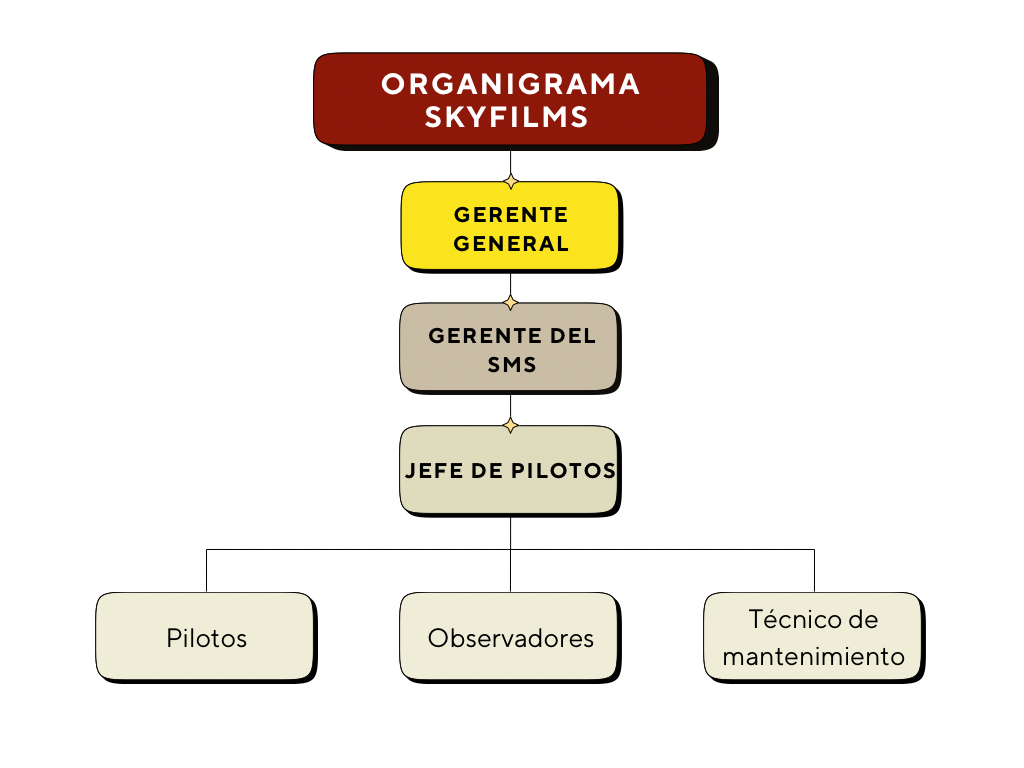
\includegraphics[width=.85\textwidth]{Imagenes/organigrama_skyfilm.PNG}
\caption{Estructura MO Skyfilms}
\end{figure}


\noindent\textbf{Nota:} La estructura organizacional presentada corresponde únicamente a la organización operacional de Skyfilms para la gestión de las operaciones UAS. Las funciones administrativas que no intervienen directamente en la operación aérea no hacen parte del presente Manual de Operaciones.

\section{Cadena de Autoridad}

La estructura de autoridad de Skyfilms S.A.S. garantiza que todas las operaciones con Sistemas de Aeronaves No Tripuladas (UAS) se desarrollen bajo una línea clara de responsabilidad, comunicación y toma de decisiones, asegurando el cumplimiento de los requisitos establecidos por la Aerocivil y por el Sistema de Gestión de la Seguridad Operacional (SMS).

La autoridad operacional se ejerce de manera jerárquica, conforme al siguiente orden:

\begin{enumerate}
    \item Gerente General.
    \item Jefe de Pilotos UAS.
    \item Pilotos Remotos.
    \item Observadores Visuales.
\end{enumerate}

El Responsable de Mantenimiento y el Gerente de Seguridad Operacional (SMS) ejercen funciones especializadas dentro de su ámbito de competencia, manteniendo independencia funcional respecto de la ejecución de las operaciones cuando así lo requiera la seguridad operacional.





\begin{table}[H]
\centering
\renewcommand{\arraystretch}{1.3}
\begin{tabularx}{\textwidth}{|p{4cm}|X|}
\hline
\textbf{Cargo} & \textbf{Nivel de autoridad} \\ \hline

Gerente General &
Máxima autoridad administrativa y operacional del explotador UAS. \\ \hline

Jefe de Pilotos UAS &
Autoriza, coordina y supervisa la ejecución de las operaciones de vuelo. \\ \hline

Gerente SMS &
Supervisa el cumplimiento de la seguridad operacional y puede recomendar la suspensión de una operación cuando identifique un riesgo no aceptable. \\ \hline

Responsable de Mantenimiento &
Autoriza la disponibilidad técnica de las aeronaves y equipos para la operación. \\ \hline

Piloto Remoto &
Responsable de la conducción segura de la aeronave durante la misión autorizada. \\ \hline

Observador Visual &
Apoya al piloto manteniendo vigilancia del entorno operacional y comunicando cualquier condición que pueda afectar la seguridad del vuelo. \\ \hline

\end{tabularx}
\caption{Cadena de autoridad operacional de Skyfilms.}
\end{table}


\section{Responsabilidades}


\subsection{Gerente General}

\subsubsection*{Objetivo del cargo}

El Gerente General es la máxima autoridad administrativa y operacional de Skyfilms S.A.S. y es responsable de garantizar que todas las operaciones con Sistemas de Aeronaves No Tripuladas (UAS) se desarrollen conforme al RAC 100, las Especificaciones Operacionales (OpSpecs), el presente Manual de Operaciones y demás normativa aplicable.

\subsubsection*{Responsabilidades}

\begin{enumerate}[label=\alph*)]
\item Aprobar el Manual de Operaciones y sus revisiones o enmiendas.
\item Garantizar la disponibilidad de recursos humanos, técnicos y financieros para la operación segura de los UAS.
\item Designar al Jefe de Pilotos UAS, al Gerente SMS y al Responsable de Mantenimiento.
\item Autorizar la incorporación de nuevas aeronaves, equipos tecnológicos y personal operativo.
\item Asegurar el cumplimiento de los requisitos establecidos por la Aerocivil.
\item Firmar las comunicaciones oficiales dirigidas a la Aerocivil.
\item Promover la cultura de seguridad operacional dentro de la organización.
\end{enumerate}

\subsubsection*{Autoridad}

El Gerente General podrá aprobar, suspender o cancelar cualquier operación cuando considere que existen condiciones que afecten la seguridad operacional, el cumplimiento normativo o los intereses de Skyfilms.

\subsubsection*{Reporta a}

No aplica.

\subsubsection*{Supervisa a}

\begin{itemize}
\item Jefe de Pilotos UAS.
\item Gerente de Seguridad Operacional (SMS).
\item Responsable de Mantenimiento.
\end{itemize}



\subsection{Jefe de Pilotos UAS}

\subsubsection*{Objetivo del cargo}

El Jefe de Pilotos UAS es el responsable de la planificación, coordinación, supervisión y control de las operaciones de vuelo desarrolladas por Skyfilms S.A.S., garantizando que todas las misiones se ejecuten de conformidad con el Reglamento Aeronáutico de Colombia (RAC 100), las Especificaciones Operacionales (OpSpecs), el presente Manual de Operaciones y demás normativa aplicable.


\subsubsection*{Responsabilidades}

Son responsabilidades del Jefe de Pilotos UAS:

\begin{enumerate}[label=\alph*)]

\item Planificar, coordinar y supervisar las operaciones UAS desarrolladas por Skyfilms.

\item Verificar que cada operación cuente con los permisos, autorizaciones y documentación exigida por la Aerocivil y demás autoridades competentes.

\item Autorizar la ejecución de las misiones de vuelo una vez verificado el cumplimiento de los requisitos operacionales, técnicos y de seguridad.

\item Asignar los pilotos remotos, observadores visuales y demás personal operativo requerido para cada misión.

\item Verificar que el personal operativo mantenga vigente su competencia, capacitación y habilitación para desempeñar sus funciones.

\item Supervisar el cumplimiento de los procedimientos establecidos en el Manual de Operaciones, Manual SMS y Manual de Control de Mantenimiento.

\item Coordinar con el Responsable de Mantenimiento la disponibilidad técnica y aeronavegabilidad de las aeronaves no tripuladas antes de cada operación.

\item Coordinar con el Gerente de Seguridad Operacional (SMS) la identificación de peligros, evaluación de riesgos y aplicación de medidas de mitigación cuando sea requerido.

\item Garantizar que los formatos operacionales, listas de chequeo, bitácoras de vuelo y demás registros sean diligenciados y archivados correctamente.

\item Supervisar el cumplimiento de los procedimientos de planificación, ejecución y cierre de las operaciones.

\item Gestionar la actualización de los registros de aeronaves, equipos tecnológicos y pilotos ante la Aerocivil cuando corresponda.

\item Participar en la investigación de incidentes, accidentes y eventos operacionales cuando sea requerido.

\item Proponer acciones de mejora para incrementar la seguridad operacional y la eficiencia de las operaciones.

\item Suspender o cancelar una operación cuando las condiciones operacionales, meteorológicas, técnicas o de seguridad no permitan garantizar un nivel aceptable de riesgo.

\end{enumerate}

\subsubsection*{Autoridad}

El Jefe de Pilotos UAS está facultado para:

\begin{itemize}

\item Autorizar el inicio de una operación UAS.

\item Suspender temporalmente una misión.

\item Cancelar una operación cuando existan condiciones inseguras.

\item Reasignar tripulaciones o aeronaves.

\item Exigir el cumplimiento de los procedimientos establecidos en el presente Manual de Operaciones.

\item Solicitar apoyo del Responsable de Mantenimiento o del Gerente SMS cuando las condiciones de la operación así lo requieran.

\end{itemize}


\textbf{Requisitos mínimos (Conforme al RAC 100.520):}
\begin{itemize}
    \item Contar con certificado vigente como Piloto UAS y capacitación en las operaciones autorizadas al explotador.
    \item Demostrar experiencia operacional de, al menos, cien (100) horas de vuelo en UAS similares a los de la flota de Skyfilms.
    \item Demostrar al menos seis (6) meses de experiencia en actividades administrativas relacionadas con operaciones en aviación no tripulada.
    \item Contar con capacitación certificada por un CIAC o CEAC de, al menos, cuarenta (40) horas en Sistema de Gestión de la Seguridad Operacional (SMS).
\end{itemize}

\subsubsection*{Reporta a}

Gerente General.

\subsubsection*{Supervisa a}

\begin{itemize}

\item Pilotos Remotos.

\item Observadores Visuales.

\end{itemize}

\begin{table}[H]
\centering
\renewcommand{\arraystretch}{1.3}
\begin{tabularx}{\textwidth}{|p{4cm}|X|}
\hline
\textbf{Cargo} & Jefe de Pilotos UAS \\ \hline
\textbf{Reporta a} & Gerente General \\ \hline
\textbf{Supervisa} & Pilotos Remotos y Observadores Visuales \\ \hline
\textbf{Autoridad} & Planificar, autorizar, supervisar, suspender y cancelar operaciones UAS. \\ \hline
\textbf{Documentos relacionados} & MO, SMS, MCM, OpSpecs y procedimientos operacionales. \\ \hline
\end{tabularx}
\caption{Resumen del cargo de Jefe de Pilotos UAS.}
\end{table}


\subsection{Gerente de Seguridad Operacional (SMS)}

\subsubsection*{Objetivo del cargo}

El Gerente de Seguridad Operacional (SMS) es el responsable de administrar, supervisar y promover el Sistema de Gestión de la Seguridad Operacional de Skyfilms S.A.S., garantizando la identificación de peligros, la gestión de riesgos y la implementación de medidas orientadas a mantener un nivel aceptable de seguridad operacional en todas las actividades relacionadas con la operación de Sistemas de Aeronaves No Tripuladas (UAS).

\subsubsection*{Responsabilidades}

Son responsabilidades del Gerente de Seguridad Operacional:

\begin{enumerate}[label=\alph*)]

\item Administrar y mantener actualizado el Sistema de Gestión de la Seguridad Operacional (SMS).

\item Identificar peligros y evaluar los riesgos asociados a las operaciones UAS.

\item Proponer e implementar medidas de mitigación para reducir los riesgos operacionales.

\item Promover la cultura de seguridad operacional dentro de la organización.

\item Realizar seguimiento a los indicadores de desempeño en seguridad operacional.

\item Gestionar el reporte voluntario y obligatorio de sucesos relacionados con la seguridad operacional.

\item Coordinar la investigación de incidentes y accidentes cuando corresponda.

\item Recomendar la suspensión de operaciones cuando identifique riesgos que superen el nivel aceptable definido por Skyfilms.

\item Verificar el cumplimiento de los procedimientos establecidos en el Manual SMS.

\item Coordinar con el Jefe de Pilotos y el Responsable de Mantenimiento la implementación de acciones correctivas y preventivas.

\item Elaborar informes periódicos sobre el desempeño del Sistema de Gestión de la Seguridad Operacional.

\end{enumerate}

\subsubsection*{Autoridad}

El Gerente de Seguridad Operacional está facultado para:

\begin{itemize}

\item Recomendar la suspensión o cancelación de una operación cuando identifique un riesgo no aceptable.

\item Solicitar la implementación inmediata de medidas de mitigación.

\item Acceder a toda la información operacional necesaria para el cumplimiento de sus funciones.

\item Solicitar investigaciones relacionadas con la seguridad operacional.

\item Presentar recomendaciones directamente al Gerente General sin necesidad de autorización previa.

\end{itemize}

\subsubsection*{Independencia funcional}

El Gerente de Seguridad Operacional ejercerá sus funciones con independencia funcional respecto de la planificación y ejecución de las operaciones UAS.

Ninguna decisión administrativa u operacional podrá limitar la presentación de reportes, recomendaciones o acciones relacionadas con la seguridad operacional.

\textbf{Requisitos mínimos (Conforme al RAC 100.520):}
\begin{itemize}
    \item Contar con un curso básico sobre SMS certificado por un CIAC o CEAC de, al menos, cuarenta (40) horas.
    \item Demostrar conocimientos o formación en áreas del sector aeronáutico.
    \item Contar con experiencia operacional aeronáutica comprobable de, al menos, doce (12) meses.
\end{itemize}

\subsubsection*{Reporta a}

Gerente General y Jefe de Piltos.

\subsubsection*{Supervisa a}

No aplica.


\begin{table}[H]
\centering
\renewcommand{\arraystretch}{1.3}

\begin{tabularx}{\textwidth}{|p{4cm}|X|}
\hline
\textbf{Cargo} & Gerente de Seguridad Operacional \\ \hline
\textbf{Reporta a} & Gerente General \\ \hline
\textbf{Supervisa} & No aplica \\ \hline
\textbf{Autoridad} & Gestionar el SMS, recomendar la suspensión de operaciones, administrar la gestión del riesgo y realizar seguimiento al desempeño de la seguridad operacional. \\ \hline
\textbf{Documentos relacionados} & Manual SMS, Manual de Operaciones, OpSpecs, procedimientos de gestión del riesgo e investigación de sucesos. \\ \hline
\end{tabularx}

\caption{Resumen del cargo de Gerente de Seguridad Operacional.}

\end{table}


\subsection{Responsable de Mantenimiento}

\subsubsection*{Objetivo del cargo}

El Responsable de Mantenimiento es el encargado de planificar, coordinar, supervisar y controlar las actividades de mantenimiento preventivo, correctivo e inspección de las aeronaves no tripuladas, baterías, estaciones de control y equipos tecnológicos utilizados por Skyfilms S.A.S., garantizando que todos los equipos se encuentren en condiciones seguras para la operación y de conformidad con el Manual de Control de Mantenimiento (MCM), las recomendaciones del fabricante y la normativa vigente.

\subsubsection*{Responsabilidades}

Son responsabilidades del Responsable de Mantenimiento:

\begin{enumerate}[label=\alph*)]

\item Elaborar y mantener actualizado el Programa de Mantenimiento de las aeronaves y equipos tecnológicos.

\item Verificar el estado de aeronavegabilidad de cada UAS antes de ser liberado para operación.

\item Ejecutar o supervisar las actividades de mantenimiento preventivo y correctivo.

\item Controlar la vida útil, ciclos de operación y estado de las baterías utilizadas por Skyfilms.

\item Mantener actualizado el historial técnico de cada aeronave, motor, batería y equipo tecnológico.

\item Garantizar que únicamente sean utilizados repuestos y componentes autorizados por el fabricante o aprobados por Skyfilms.

\item Coordinar con el Jefe de Pilotos la disponibilidad técnica de las aeronaves para las operaciones programadas.

\item Informar inmediatamente cualquier condición técnica que pueda afectar la seguridad operacional.

\item Suspender la disponibilidad operacional de cualquier aeronave que presente una condición insegura.

\item Mantener actualizados los registros de mantenimiento, inspecciones y reparaciones.

\item Verificar que las herramientas y equipos de mantenimiento se encuentren en condiciones adecuadas de uso.

\item Coordinar el envío de equipos a talleres especializados cuando las reparaciones excedan las capacidades técnicas de Skyfilms.

\end{enumerate}


\subsubsection*{Autoridad}

El Responsable de Mantenimiento está facultado para:

\begin{itemize}

\item Declarar una aeronave apta para operación.

\item Restringir o suspender la utilización de una aeronave o equipo tecnológico cuando exista una condición que afecte su aeronavegabilidad.

\item Programar inspecciones extraordinarias.

\item Solicitar mantenimiento preventivo o correctivo en cualquier momento.

\item Recomendar el retiro definitivo de equipos que no garanticen condiciones seguras de operación.

\end{itemize}


\subsubsection*{Requisitos mínimos}

El Responsable de Mantenimiento deberá:

\begin{itemize}

\item Conocer el Manual de Control de Mantenimiento (MCM).

\item Conocer las recomendaciones técnicas de los fabricantes de las aeronaves y equipos utilizados por Skyfilms.

\item Demostrar competencias en mantenimiento de sistemas UAS.

\item Mantener vigente la capacitación definida por Skyfilms para el desempeño de sus funciones.

\end{itemize}


\subsubsection*{Reporta a}

Gerente General.


\subsubsection*{Supervisa a}

Personal técnico de mantenimiento o proveedores autorizados que ejecuten actividades de mantenimiento para Skyfilms.

\begin{table}[H]
\centering
\renewcommand{\arraystretch}{1.3}

\begin{tabularx}{\textwidth}{|p{4cm}|X|}
\hline
\textbf{Cargo} & Responsable de Mantenimiento \\ \hline
\textbf{Reporta a} & Gerente General \\ \hline
\textbf{Supervisa} & Técnicos de mantenimiento o proveedores autorizados \\ \hline
\textbf{Autoridad} & Liberar, restringir o suspender la disponibilidad técnica de aeronaves y equipos. \\ \hline
\textbf{Documentos relacionados} & Manual de Control de Mantenimiento (MCM), Manual de Operaciones, Manuales del fabricante y registros técnicos. \\ \hline
\end{tabularx}

\caption{Resumen del cargo de Responsable de Mantenimiento.}

\end{table}



\subsection{Piloto Remoto UAS}

\subsubsection*{Objetivo del cargo}

El Piloto Remoto UAS es el responsable de la conducción segura de la aeronave no tripulada durante todas las fases de la operación, garantizando el cumplimiento del presente Manual de Operaciones, las Especificaciones Operacionales (OpSpecs), el Reglamento Aeronáutico de Colombia (RAC 100) y los procedimientos establecidos por Skyfilms S.A.S.


\subsubsection*{Responsabilidades}

Son responsabilidades del Piloto Remoto UAS:

\begin{enumerate}[label=\alph*)]

\item Ejecutar las operaciones de vuelo autorizadas conforme a la planificación aprobada.

\item Verificar el cumplimiento del checklist previo al vuelo antes de iniciar cualquier operación.

\item Confirmar que la aeronave, estación de control, baterías y equipos asociados se encuentren en condiciones seguras para la operación.

\item Mantener el control de la aeronave durante toda la misión.

\item Cumplir las limitaciones operacionales establecidas en las OpSpecs y en el presente Manual.

\item Mantener comunicación permanente con el Observador Visual cuando la operación así lo requiera.

\item Interrumpir o abortar la misión cuando identifique una condición que comprometa la seguridad operacional.

\item Registrar la información correspondiente en la bitácora de vuelo al finalizar cada operación.

\item Reportar cualquier incidente, accidente o condición insegura al Jefe de Pilotos y al Gerente SMS.

\item Cumplir las instrucciones emitidas por el Jefe de Pilotos y las recomendaciones de seguridad operacional emitidas por el Gerente SMS.

\end{enumerate}


\subsubsection*{Autoridad}

El Piloto Remoto está facultado para:

\begin{itemize}

\item Interrumpir inmediatamente una operación cuando identifique condiciones inseguras.

\item Declarar una situación de emergencia operacional.

\item Solicitar apoyo del Observador Visual o del Jefe de Pilotos durante la misión.

\item Negarse a iniciar una operación cuando considere que no existen condiciones seguras para realizarla.

\end{itemize}


\subsubsection*{Requisitos mínimos}

El Piloto Remoto deberá:

\begin{itemize}

\item Contar con certificado vigente como Piloto Remoto UAS conforme al RAC 100.

\item Mantener vigente la capacitación operacional establecida por Skyfilms.

\item Conocer el Manual de Operaciones, el Manual SMS y los procedimientos de emergencia.

\item Mantener la competencia operacional para el tipo de aeronave que opera.

\end{itemize}

\subsubsection*{Reporta a}

Jefe de Pilotos UAS.

\begin{table}[H]
\centering
\renewcommand{\arraystretch}{1.3}

\begin{tabularx}{\textwidth}{|p{4cm}|X|}
\hline
\textbf{Cargo} & Piloto Remoto UAS \\ \hline
\textbf{Reporta a} & Jefe de Pilotos UAS \\ \hline
\textbf{Autoridad} & Ejecutar, suspender o abortar la operación cuando la seguridad operacional lo requiera. \\ \hline
\textbf{Documentos relacionados} & Manual de Operaciones, Manual SMS, OpSpecs, listas de chequeo y procedimientos de emergencia. \\ \hline
\end{tabularx}

\caption{Resumen del cargo de Piloto Remoto UAS.}

\end{table}

\subsection{Observador Visual}

\subsubsection*{Objetivo del cargo}

El Observador Visual es el responsable de mantener vigilancia permanente sobre la aeronave no tripulada y su entorno operacional durante la ejecución de la misión, apoyando al Piloto Remoto mediante la identificación oportuna de riesgos, obstáculos, tráfico aéreo y cualquier condición que pueda afectar la seguridad operacional.

\subsubsection*{Responsabilidades}

Son responsabilidades del Observador Visual:

\begin{enumerate}[label=\alph*)]

\item Mantener contacto visual permanente con la aeronave cuando la operación así lo requiera.

\item Informar inmediatamente al Piloto Remoto sobre cualquier condición que pueda afectar la seguridad del vuelo.

\item Vigilar la presencia de personas, vehículos, obstáculos y otras aeronaves dentro del área de operación.

\item Apoyar el cumplimiento de las limitaciones operacionales establecidas para la misión.

\item Mantener comunicación efectiva con el Piloto Remoto durante toda la operación.

\item En operaciones FPV, mantener el contacto visual directo (VLOS) ininterrumpido con la aeronave para compensar la visión limitada del Piloto Remoto que utiliza las gafas FPV.

\item Colaborar en la aplicación de los procedimientos de emergencia cuando sea requerido.

\item Reportar condiciones inseguras observadas durante la operación.

\end{enumerate}

\subsubsection*{Autoridad}

El Observador Visual está facultado para:

\begin{itemize}

\item Solicitar al Piloto Remoto la interrupción inmediata de una operación cuando identifique una condición que represente un riesgo para la seguridad.

\item Recomendar modificaciones en la operación cuando observe condiciones que puedan afectar el desarrollo seguro de la misión.

\end{itemize}

\subsubsection*{Requisitos mínimos}

El Observador Visual deberá:

\begin{itemize}

\item Haber recibido la capacitación establecida por Skyfilms para el desempeño de sus funciones.

\item Conocer el presente Manual de Operaciones y los procedimientos de emergencia.

\item Mantener comunicación permanente con el Piloto Remoto durante las operaciones.

\end{itemize}


\subsubsection*{Reporta a}

Jefe de Pilotos UAS.

\begin{table}[H]
\centering
\renewcommand{\arraystretch}{1.3}

\begin{tabularx}{\textwidth}{|p{4cm}|X|}
\hline
\textbf{Cargo} & Observador Visual \\ \hline
\textbf{Reporta a} & Jefe de Pilotos UAS \\ \hline
\textbf{Autoridad} & Recomendar la interrupción de la operación cuando identifique condiciones inseguras. \\ \hline
\textbf{Documentos relacionados} & Manual de Operaciones, listas de chequeo y procedimientos de emergencia. \\ \hline
\end{tabularx}

\caption{Resumen del cargo de Observador Visual.}

\end{table}



\section{Matriz de Responsabilidades Operacionales (RACI)}

La presente matriz define la asignación de responsabilidades para los principales procesos operacionales desarrollados por Skyfilms S.A.S., permitiendo establecer de manera clara la autoridad, ejecución, consulta e información requerida para cada actividad.

Para efectos de la presente matriz se adoptan las siguientes convenciones:

\begin{itemize}
\item \textbf{R (Responsible):} Responsable directo de ejecutar la actividad.
\item \textbf{A (Accountable):} Responsable de aprobar o asumir la responsabilidad final del proceso.
\item \textbf{C (Consulted):} Debe ser consultado antes de ejecutar la actividad.
\item \textbf{I (Informed):} Debe ser informado del resultado o estado de la actividad.
\end{itemize}

\renewcommand{\arraystretch}{1.4}

\scriptsize

\begin{longtable}{|p{6.5cm}|c|c|c|c|c|c|}
\hline

\textbf{Actividad} &
\rotatebox{90}{Gerente} &
\rotatebox{90}{Jefe de Pilotos} &
\rotatebox{90}{SMS} &
\rotatebox{90}{Mantenimiento} &
\rotatebox{90}{Piloto} &
\rotatebox{90}{Observador}
\\
\hline
\endhead

Planificación de la misión &
I &
A &
C &
C &
R &
I
\\ \hline

Evaluación del riesgo operacional &
I &
C &
A/R &
C &
C &
C
\\ \hline

Autorización de la operación &
A &
R &
C &
C &
I &
I
\\ \hline

Verificación documental &
I &
A &
I &
C &
R &
I
\\ \hline

Liberación técnica del UAS &
I &
C &
I &
A/R &
I &
I
\\ \hline

Inspección preoperacional &
I &
C &
I &
C &
A/R &
R
\\ \hline

Ejecución del vuelo &
I &
I &
I &
I &
A/R &
R
\\ \hline

Gestión de emergencia &
I &
A &
C &
C &
R &
R
\\ \hline

Reporte de incidente &
I &
C &
A &
I &
R &
R
\\ \hline

Investigación de incidente &
I &
C &
A/R &
C &
C &
C
\\ \hline

Control de registros operacionales &
I &
A &
I &
I &
R &
I
\\ \hline

Control de mantenimiento &
I &
I &
I &
A/R &
C &
I
\\ \hline

Programación de mantenimiento &
I &
C &
I &
A/R &
I &
I
\\ \hline

Actualización del Manual &
A &
C/R &
C/R &
C &
I &
I
\\ \hline

Capacitación del personal &
A &
R &
C/R&
C &
I &
I
\\ \hline

\caption{Matriz RACI de responsabilidades operacionales de Skyfilms.}

\end{longtable}


\begin{tcolorbox}[title=Interpretación de la matriz]

Cuando una actividad presente simultáneamente un responsable de aprobación (A) y un responsable de ejecución (R), la actividad únicamente podrá considerarse finalizada cuando ambas responsabilidades hayan sido cumplidas.

La asignación de responsabilidades establecida en la presente matriz no exime a ningún integrante de Skyfilms del deber de informar cualquier condición que pueda afectar la seguridad operacional.

\end{tcolorbox}


\section{Sustitución temporal y delegación de funciones}

Con el fin de garantizar la continuidad de las operaciones y mantener el cumplimiento de los requisitos establecidos por el Reglamento Aeronáutico de Colombia (RAC 100), Skyfilms S.A.S. establece el presente procedimiento para la sustitución temporal de cargos y la delegación de funciones cuando un responsable no pueda ejercer sus funciones por ausencia, incapacidad, vacaciones, comisión de servicio o cualquier otra circunstancia que impida el normal desarrollo de sus actividades.

La delegación de funciones no exime al titular del cargo de las responsabilidades que le correspondan cuando reasuma sus funciones, ni modifica las responsabilidades asignadas a los demás integrantes de la organización.


\subsection*{Principios generales}

La sustitución temporal de cargos se regirá por los siguientes principios:

\begin{enumerate}[label=\alph*)]

\item La continuidad operacional no deberá verse afectada por la ausencia temporal de un responsable.

\item Ninguna persona podrá asumir funciones para las cuales no haya sido previamente designada y demostrada su competencia.

\item La delegación deberá quedar documentada cuando implique decisiones operacionales o administrativas relevantes.

\item Las funciones relacionadas con la seguridad operacional conservarán la independencia funcional establecida en el Sistema de Gestión de la Seguridad Operacional (SMS).

\end{enumerate}

\renewcommand{\arraystretch}{1.4}

\begin{longtable}{|p{4cm}|p{5cm}|p{5cm}|}

\hline

\textbf{Cargo} &
\textbf{Sustituto temporal} &
\textbf{Condición para asumir el cargo}

\\ \hline

Gerente General &
Jefe de Pilotos UAS &
Cuando exista delegación expresa del Gerente General.

\\ \hline

Jefe de Pilotos UAS &
Piloto Remoto designado por la Gerencia &
Debe cumplir los requisitos establecidos para el cargo y ser designado formalmente.

\\ \hline

Gerente SMS &
Profesional designado por la Gerencia con competencias en SMS &
Debe conservar la independencia funcional respecto de la operación.

\\ \hline

Responsable de Mantenimiento &
Técnico competente o proveedor autorizado &
Debe demostrar competencia para ejecutar las actividades delegadas.

\\ \hline

Piloto Remoto &
Otro Piloto Remoto habilitado &
Debe encontrarse vigente y autorizado para operar el tipo de aeronave correspondiente.

\\ \hline

Observador Visual &
Otro Observador Visual capacitado &
Debe haber recibido la capacitación establecida por Skyfilms.

\\ \hline

\caption{Sustitución temporal de cargos operacionales.}

\end{longtable}


\subsection*{Ejercicio simultáneo de cargos}

Durante la etapa inicial de operación de Skyfilms S.A.S., una misma persona podrá ejercer simultáneamente los cargos de Gerente General y Jefe de Pilotos UAS, siempre que:

\begin{enumerate}[label=\alph*)]

\item Se garantice el cumplimiento integral de las responsabilidades asignadas a ambos cargos.

\item No se comprometa la seguridad operacional.

\item Se mantenga la independencia funcional del Gerente de Seguridad Operacional (SMS).

\item Se conserve la adecuada supervisión de las actividades de mantenimiento.

\end{enumerate}


\subsection*{Delegación de autoridad}

Cuando un responsable delegue temporalmente sus funciones deberá garantizar, como mínimo:

\begin{itemize}

\item La entrega de la información necesaria para la continuidad de las operaciones.

\item La comunicación al personal involucrado.

\item La actualización de los registros correspondientes.

\item La conservación de la trazabilidad documental de la delegación.

\end{itemize}


\section{Coordinación entre las áreas operacionales}

Con el fin de garantizar la ejecución segura, eficiente y conforme a la reglamentación vigente de todas las operaciones UAS, Skyfilms establece mecanismos permanentes de coordinación entre las áreas de Operaciones, Seguridad Operacional (SMS), Mantenimiento y Gerencia General.

La coordinación entre las diferentes áreas se desarrolla durante todas las fases de la operación, desde la planificación de la misión hasta el cierre documental de la misma.



\renewcommand{\arraystretch}{1.4}

\begin{longtable}{|p{4cm}|p{5cm}|p{6cm}|}

\hline

\textbf{Área} &
\textbf{Coordina con} &
\textbf{Objeto de la coordinación}

\\ \hline

Gerencia General &
Todas las áreas &
Disponibilidad de recursos, aprobación de políticas y toma de decisiones estratégicas.

\\ \hline

Jefe de Pilotos &
SMS y Mantenimiento &
Planificación de operaciones, disponibilidad técnica, gestión del riesgo y asignación de tripulaciones.

\\ \hline

SMS &
Operaciones y Mantenimiento &
Identificación de peligros, mitigación de riesgos, investigación de incidentes y seguimiento de acciones correctivas.

\\ \hline

Mantenimiento &
Operaciones &
Disponibilidad técnica de aeronaves, inspecciones, mantenimiento preventivo y correctivo.

\\ \hline

Piloto Remoto &
Observador Visual &
Ejecución segura de la misión, comunicaciones y aplicación de procedimientos de emergencia.

\\ \hline

\caption{Coordinación entre las áreas operacionales de Skyfilms.}

\end{longtable}



















\section{Sistema y Procedimiento para el Control y Supervisión de las Operaciones UAS}

Skyfilms implementa un sistema de control y supervisión basado en la estandarización de procedimientos, el uso de listas de verificación operacionales y la designación clara de responsables en cada fase de la operación. Este sistema asegura que todas las misiones se ejecuten de conformidad con el Manual de Operaciones y las disposiciones establecidas por la Aerocivil.

\subsection*{Control de las operaciones}
El control de las operaciones se realiza a través de los siguientes elementos:
\begin{itemize}
    \item Diligenciamiento obligatorio de formatos de solicitud y autorización de vuelo, conforme a los requisitos de la Aerocivil.
    \item Aplicación de listas de verificación de pre-vuelo, vuelo y post-vuelo, supervisadas por el Jefe de Pilotos.
    \item Registro de horas de vuelo, aeronaves utilizadas, pilotos responsables y observadores asignados en la bitácora oficial de Skyfilms.
    \item Reporte inmediato de incidentes, anomalías o desviaciones operacionales al Gerente de Seguridad Operacional.
\end{itemize}

\subsection*{Supervisión de las operaciones}
La supervisión se articula a través de las siguientes responsabilidades:
\begin{itemize}
    \item El \textbf{Jefe de Pilotos} supervisa la correcta ejecución de cada operación, revisando planes de vuelo, asignación de recursos y cumplimiento de checklists.
    \item El \textbf{Gerente de Seguridad Operacional} monitorea el cumplimiento de las normas de seguridad operacional, analiza reportes de incidentes y propone medidas de mitigación.
    \item El \textbf{Gerente General} garantiza que los informes de supervisión sean presentados ante la Aerocivil cuando así se requiera.
\end{itemize}

\subsection*{Procedimiento}
El procedimiento para el control y la supervisión de las operaciones se desarrolla de la siguiente manera:
\begin{enumerate}
    \item El piloto presenta la solicitud de operación al Jefe de Pilotos con la información requerida.
    \item El Jefe de Pilotos valida la documentación, aprueba la operación y designa tripulación y recursos.
    \item Durante el vuelo, el piloto y observador/es siguen las listas de verificación operacionales, bajo la supervisión directa del Jefe de Pilotos.
    \item Al finalizar la operación, el piloto completa el registro de vuelo y el Técnico UAS realiza la inspección post-vuelo de la aeronave.
    \item El Gerente de Seguridad Operacional revisa los reportes de cada misión, consolida hallazgos y los comunica al Gerente General.
    \item En caso de incidentes, el Gerente de Seguridad Operacional inicia el proceso de análisis y emite las recomendaciones correspondientes.
\end{enumerate}



\section{Integración del Sistema de Gestión Operacional}

La estructura organizacional definida en el presente capítulo constituye la base del Sistema de Gestión Operacional de Skyfilms S.A.S.

Las funciones, responsabilidades, competencias y mecanismos de coordinación establecidos para cada cargo se complementan con los procedimientos operacionales, el Sistema de Gestión de la Seguridad Operacional (SMS), el Manual de Control de Mantenimiento (MCM), las Especificaciones Operacionales (OpSpecs) y los formatos controlados de la organización.

El control y supervisión de las operaciones UAS se ejerce mediante:

\begin{itemize}

\item La estructura organizacional.

\item La cadena de autoridad.

\item La Matriz RACI.

\item Los procedimientos operacionales.

\item Las listas de chequeo.

\item Los registros de vuelo.

\item Los procesos de mantenimiento.

\item El Sistema de Gestión de la Seguridad Operacional.

\end{itemize}

\section{Instalaciones Administrativas y Operativas}
La sede administrativa y de coordinación de operaciones de Skyfilms S.A.S. se encuentra ubicada en la ciudad de Ibagué, Tolima, desde donde se centraliza la planificación de los vuelos, el control documental, el resguardo de la biblioteca técnica y la gestión de la seguridad operacional (SMS).

Debido a la naturaleza de la producción audiovisual, Skyfilms no opera desde bases fijas de lanzamiento. Las zonas de operación (Dronpuertos) son de carácter móvil y temporal, estableciéndose en los lugares de rodaje específicos de acuerdo con la planificación de cada misión, los permisos obtenidos y las condiciones de seguridad estipuladas en el presente manual. El almacenamiento de las aeronaves y baterías se realiza en la base principal bajo condiciones controladas de temperatura y humedad, aisladas de personal no autorizado.

\label{fin_cap2} %

% Capítulo 3: Operaciones UAS

\chapter{Operaciones UAS}
\label{chap:operaciones}
\section{Filosofía operacional}
\label{inicio_cap3}

Skyfilms S.A.S. desarrolla operaciones con Sistemas de Aeronaves No Tripuladas (UAS) bajo un modelo de gestión orientado a la seguridad operacional, la estandarización de procedimientos y la mejora continua.

Todas las operaciones son planificadas, ejecutadas y supervisadas conforme a los requisitos establecidos en el Reglamento Aeronáutico de Colombia (RAC 100), las Especificaciones Operacionales (OpSpecs), el presente Manual de Operaciones, el Sistema de Gestión de la Seguridad Operacional (SMS) y el Manual de Control de Mantenimiento (MCM).

La seguridad operacional constituye el principio rector de todas las actividades desarrolladas por Skyfilms. En consecuencia, ninguna misión tendrá prioridad sobre la protección de las personas, la preservación de los bienes, el cumplimiento de la reglamentación aeronáutica o la integridad de las aeronaves y equipos utilizados.

\subsection{Principios operacionales}

Las operaciones desarrolladas por Skyfilms se fundamentan en los siguientes principios:

\begin{enumerate}[label=\arabic*.]

\item La seguridad operacional prevalece sobre cualquier objetivo comercial, operativo o contractual.

\item Ninguna operación será ejecutada sin una adecuada planificación y evaluación previa de los riesgos.

\item Toda misión deberá ser autorizada conforme a los procedimientos establecidos por la organización.

\item Todo el personal involucrado deberá conocer claramente sus funciones, responsabilidades y autoridad antes del inicio de la operación.

\item Las aeronaves únicamente serán utilizadas cuando se encuentren en condiciones técnicas adecuadas para la operación.

\item Todas las operaciones deberán generar registros documentales que permitan demostrar su planificación, ejecución y cierre.

\item Todo incidente, accidente o condición insegura será reportado y gestionado conforme al Sistema de Gestión de la Seguridad Operacional (SMS).

\item Skyfilms promoverá la mejora continua mediante el análisis de la información operacional, la retroalimentación del personal y la actualización permanente de sus procedimientos.
\end{enumerate}


\subsection{Objetivos operacionales}

Las operaciones UAS desarrolladas por Skyfilms tienen como objetivos principales:

\begin{itemize}

\item Garantizar operaciones seguras y conformes con la reglamentación aeronáutica.

\item Proteger la integridad de las personas, bienes y aeronaves.

\item Obtener productos audiovisuales de alta calidad para los clientes.

\item Mantener un elevado nivel de profesionalismo en todas las operaciones.

\item Fortalecer la cultura de seguridad operacional dentro de la organización.

\item Promover la mejora continua de los procesos operacionales.

\end{itemize}


\begin{tcolorbox}[title=Política Operacional de Skyfilms,colback=gray!5,colframe=black]

Skyfilms S.A.S. se compromete a desarrollar operaciones UAS bajo los más altos estándares de seguridad operacional, cumplimiento normativo y profesionalismo, promoviendo una cultura organizacional basada en la planificación, la gestión del riesgo, la disciplina operacional y la mejora continua.

Toda decisión operacional deberá orientarse a preservar la seguridad de las personas, proteger el espacio aéreo y garantizar la confianza de nuestros clientes y de la autoridad aeronáutica.

\end{tcolorbox}




\section{Flota UAS}
Skyfilms S.A.S. operará la siguiente flota, sujeta a los procesos de adquisición y registro formal ante la Aerocivil.

\subsection{Ficha Técnica: DJI Mavic 4 Pro}
\begin{table}[H]
    \centering
    \renewcommand{\arraystretch}{1.2}
    \begin{tabular}{|p{5cm}|p{9cm}|}
        \hline
        \rowcolor[gray]{0.9} \textbf{Parámetro} & \textbf{Especificación} \\ \hline
        \textbf{Marca / Modelo} & DJI / Mavic 4 Pro \\ \hline
        \textbf{Número de Serie / RUAS} & En proceso de adquisición \\ \hline
        \textbf{MTOW (Peso al despegue)} & 1085 g (MTOM según el Manual de usuario DJI Mavic 4 Pro, v1.0, p. 93) \\ \hline
        \textbf{Dimensiones} & 347 x 283 x 107 mm (desplegado) \\ \hline
        \textbf{Clasificación / Tipo de vuelo} & Multirrotor / VTOL (Despegue y aterrizaje vertical) \\ \hline
        \textbf{Velocidad máx. (Ascenso/Descenso/Vuelo)} & 8 m/s / 6 m/s / 21 m/s \\ \hline
        \textbf{Techo máx. de operación} & 6000 m s.n.m. \\ \hline
        \textbf{Autonomía / Radio de acción} & 43 minutos (sin viento); tiempo máximo de vuelo planificado: 80\,\% de la autonomía (RAC 100.210 k) / Hasta 750 m (Restricción VLOS) \\ \hline
        \textbf{Resistencia al viento / Temp.} & 12 m/s / -10°C a 40°C \\ \hline
        \textbf{Sistemas GNSS} & GPS + Galileo + BeiDou \\ \hline
        \textbf{Protección IP} & N/A \\ \hline
        \textbf{Frecuencias / Sistema C2} & 2.4 GHz y 5.8 GHz / DJI O4 (OcuSync 4) \\ \hline
        \textbf{Latencia / Encriptación} & Aprox. 120 ms / AES-256 \\ \hline
        \textbf{Detección de obstáculos} & Omnidireccional (APAS 5.0) \\ \hline
        \textbf{Carga útil / Cámara} & Sensor Hasselblad CMOS integrado \\ \hline
        \textbf{Fuente de energía} & Batería inteligente Li-ion \\ \hline
    \end{tabular}
\end{table}

\subsection{Ficha Técnica: BetaFPV Pavo20 Pro (FPV)}
\begin{table}[H]
    \centering
    \renewcommand{\arraystretch}{1.2}
    \begin{tabular}{|p{5cm}|p{9cm}|}
        \hline
        \rowcolor[gray]{0.9} \textbf{Parámetro} & \textbf{Especificación} \\ \hline
        \textbf{Marca / Modelo} & BetaFPV / Pavo20 Pro (cinewhoop FPV de 2,2 pulgadas) \\ \hline
        \textbf{Número de Serie / RUAS} & En proceso de adquisición (Serie de FC) \\ \hline
        \textbf{MTOW (Peso al despegue)} & Por pesar: aeronave lista para volar con batería, receptor y tira LED. Referencia del fabricante: 116 g sin batería, con transmisor DJI O4 Pro \\ \hline
        \textbf{Dimensiones} & Distancia entre ejes de 93,9 mm; hélices de 2,2 pulgadas de 3 palas. Medida D (con hélices): por medir, aprox. 0,15 m \\ \hline
        \textbf{Clasificación / Tipo de vuelo} & Multirrotor FPV / VTOL \\ \hline
        \textbf{Velocidad máx. (Ascenso/Descenso/Vuelo)} & Por determinar en vuelos de prueba (modo Acro) \\ \hline
        \textbf{Techo máx. de operación} & Por confirmar (límite operacional del manual: 400 ft AGL) \\ \hline
        \textbf{Autonomía / Radio de acción} & 8 a 10 min según batería (datos del fabricante con baterías 4S de 580 a 680 mAh); tiempo máximo de vuelo planificado: 80\,\% de la autonomía / Hasta 750 m (Restricción VLOS con observador) \\ \hline
        \textbf{Resistencia al viento / Temp.} & Por determinar en vuelos de prueba \\ \hline
        \textbf{Sistemas GNSS} & Módulo GPS externo (no incluido de fábrica): modelo por confirmar \\ \hline
        \textbf{Protección IP} & Sin certificación IP \\ \hline
        \textbf{Frecuencias / Sistema C2} & ELRS XBand (Gemini Xrossband) 2.4 GHz y 915 MHz (control) / 5.8 GHz (video DJI O4 Pro) \\ \hline
        \textbf{Latencia / Encriptación} & Por medir en la demostración del enlace C2 / Salto de frecuencia y frase de enlace (\textit{binding phrase}) de ExpressLRS \\ \hline
        \textbf{Detección de obstáculos} & N/A (Vuelo visual manual 100\%) \\ \hline
        \textbf{Carga útil / Cámara} & Cámara DJI O4 Pro integrada + tira LED blanca \\ \hline
        \textbf{Fuente de energía} & Batería LiPo 3S/4S externa (580 a 680 mAh, conector XT30) \\ \hline
    \end{tabular}
\end{table}

\subsection{Equipos Tecnológicos Asociados (ETA)}
Los equipos tecnológicos no integrados de fábrica pero asociados a la operación serán declarados ante la Aerocivil.

\begin{table}[H]
    \centering
    \renewcommand{\arraystretch}{1.2}
    \begin{tabular}{|p{3cm}|p{3.5cm}|p{3.5cm}|p{4cm}|}
        \hline
        \rowcolor[gray]{0.9} \textbf{Tipo de ETA} & \textbf{Marca / Modelo} & \textbf{Serie / Registro} & \textbf{Uso / Limitación} \\ \hline
        Radiocontrol & RadioMaster TX16S (ELRS) & En proceso & Enlace C2 del Pavo20 Pro. \\ \hline
        Módulo y receptor ELRS & ELRS XBand (Gemini Xrossband), modelo por confirmar & En proceso & Control del Pavo20 Pro en 2.4 GHz y 915 MHz. \\ \hline
        Visor FPV & DJI Goggles 2 & En proceso & Visualización en tiempo real. Uso exclusivo con Observador VLOS. \\ \hline
        Tira LED & Tira LED blanca, modelo por confirmar & En proceso & Iluminación de la aeronave FPV en vuelo nocturno. \\ \hline
        Control remoto del Mavic 4 Pro y dispositivo móvil & Control DJI y dispositivo con DJI Fly, modelos por confirmar & En proceso & Estación de control del Mavic 4 Pro. \\ \hline
    \end{tabular}
\end{table}

\subsection{Software Utilizado}
\begin{itemize}
    \item \textbf{DJI Fly:} App principal para el Mavic 4 Pro. Versión actualizada oficial. Licencia gratuita. Controla telemetría, límites de vuelo y RTH.
    \item \textbf{Betaflight Configurator:} Software de código abierto utilizado exclusivamente en tierra para la configuración, tuning y asignación de failsafe (RTH por GPS) de la controladora del dron FPV.
    \item \textbf{UAV Forecast:} App meteorológica para verificación de viento, ráfagas, satélites y KP Index en locación.
\end{itemize}

\subsection{Descripción del Enlace C2}
El enlace C2 es el medio primario de comando y control. Sus especificaciones por aeronave son:
\begin{itemize}
    \item \textbf{DJI Mavic 4 Pro (DJI O4):} Opera en bandas de 2.4 GHz y 5.8 GHz con conmutación automática anti-interferencias. Encriptación AES-256. Failsafe configurado para retornar al punto de origen (RTH) tras 3 segundos de pérdida de señal.
    \item \textbf{BetaFPV Pavo20 Pro (FPV):} El control opera bajo el protocolo de código abierto ExpressLRS con receptor XBand (Gemini Xrossband) en 2.4 GHz y 915 MHz, con salto de frecuencia; el video se transmite en 5.8 GHz mediante DJI O4 Pro. La telemetría incluye LQ (Link Quality) y RSSI. El Failsafe está configurado a través de Betaflight para activar rescate por GPS (RTH) ante la desconexión total del radio control. La banda de 915 MHz se empleará únicamente cuando se confirme su uso libre ante la ANE; mientras tanto el equipo opera en 2.4 GHz.
\end{itemize}



\section{Registro UAS}


Skyfilms garantiza el cumplimiento de los procedimientos de registro de sus aeronaves no tripuladas y de los equipos tecnológicos que apoyan sus operaciones, conforme a lo establecido por la Aerocivil. Para tal fin, se aplican las siguientes disposiciones:

\begin{enumerate}[label=\alph*)]
    \item El \textbf{Jefe de Pilotos UAS} tiene la responsabilidad de adelantar el trámite de registro de cada aeronave no tripulada operada por Skyfilms, asegurando que la información presentada sea precisa, completa y actualizada.
    \item En el evento en que alguna aeronave no tripulada o sistema UAS de Skyfilms deba ser retirado por término de vida útil, pérdida de capacidad operativa, hurto o cualquier otra circunstancia que imposibilite su uso, el Jefe de Pilotos informará a la Aerocivil con el fin de formalizar la cancelación del registro correspondiente.
    \item Todo equipo tecnológico asociado a las operaciones de Skyfilms deberá ser reportado a la Aerocivil en el momento de su registro inicial o cuando se incorpore posteriormente a las misiones de vuelo.
\end{enumerate}

\subsubsection{Procedimiento para registro de aeronaves no tripuladas}

El \textbf{Jefe de Pilotos UAS de Skyfilms} es el responsable de gestionar el registro de cada aeronave no tripulada y de los equipos tecnológicos asociados, conforme a la circular informativa MAUT-5.0-22-010 “Guía para el registro de sistemas de aeronaves no tripuladas UAS y/o equipos tecnológicos en cumplimiento de la norma RAC 100”. El procedimiento comprende:

\begin{enumerate}
    \item Descargar y diligenciar, de forma individual por cada aeronave, el formato \textit{Solicitud de Registro de UAS}, que incluye la guía de diligenciamiento y el listado de anexos requeridos. Los formatos oficiales están disponibles en el portal de la Aerocivil: \texttt{www.aerocivil.gov.co}.
    \item Radicar la solicitud ante la Aerocivil a través del sitio oficial: 
    \\ \texttt{https://aerocivilsgdea.com/ControlPQR/Formulario} o mediante la opción \textit{PQRD} \textrightarrow{} \textit{PQRSD Web}.
    \item En el tipo de trámite, seleccionar \textit{Solicitud de registro o retiro de pilotos UAS, equipos tecnológicos y explotadores UAS}, adjuntando el formato diligenciado y la totalidad de documentos exigidos.
    \item Conservar el número de radicación generado por el sistema para seguimiento del estado del trámite.
    \item Una vez verificada la solicitud y cumplidos los requisitos, la Aerocivil expedirá el \textit{Certificado de Registro UAS}.
    \item El certificado emitido tendrá un número único asociado al serial de la aeronave y será intransferible.
    \item Incorporar el número de registro en la etiqueta de identificación de la aeronave, tomar una fotografía de dicha etiqueta y enviarla al correo \texttt{gdmua@aerocivil.gov.co}, indicando en el asunto el mismo número de registro.
    \item El proceso de registro se considerará finalizado cuando la Aerocivil acuse recibido de la fotografía para su archivo institucional.
\end{enumerate}

\subsubsection{Etiquetas de las aeronaves no tripuladas}

Todas las aeronaves no tripuladas registradas por \textbf{Skyfilms} en la base de datos oficial de la Aerocivil, y habilitadas para realizar operaciones aéreas, deberán portar de manera visible y permanente en su estructura una \textbf{etiqueta de identificación} con la siguiente información:

\begin{enumerate}[label=\alph*)]
    \item Número de Registro RUAS asignado por la Aerocivil.
    \item Nombre o razón social del explotador: ``Skyfilms S.A.S.''.
    \item Correo electrónico de contacto del explotador: \texttt{skyfilmsfpv@gmail.com}.
    \item Correo electrónico institucional de la Aerocivil: \texttt{atencionalciudadano@aerocivil.gov.co}.
\end{enumerate}


\subsubsection{Condiciones de la etiqueta}

Las aeronaves no tripuladas operadas por \textbf{Skyfilms} deberán portar de manera visible y permanente una etiqueta de identificación oficial, la cual debe cumplir con las siguientes condiciones:

\begin{enumerate}[label=\alph*)]
    \item Estar adherida de manera permanente a la estructura de la aeronave no tripulada.
    \item Garantizar la legibilidad permanente de toda la información consignada.
    \item No afectar el peso, balance ni el desempeño operacional de la aeronave.
    \item Ser ubicada en la superficie exterior de la aeronave, en un punto claramente visible en todo momento.
    \item Mantener un contraste de color adecuado que facilite su lectura.
\end{enumerate}

La etiqueta incluirá el número de registro RUAS asignado por la Aerocivil, el nombre del explotador \textbf{Skyfilms}, el correo electrónico de contacto de la compañía y el correo institucional de la Aerocivil.

% --- PREÁMBULO (en tu main.tex) ---
 % opcional, para iconos de correo/teléfono

% Colores corporativos (ajusta si quieres)
\definecolor{skyblack}{RGB}{20,20,20}
\definecolor{skygray}{RGB}{85,85,85}

% ---  INSERTAR LA ETIQUETA ---
\begin{figure}[H]
\centering
\begin{tcolorbox}[
    enhanced,
    width=9cm,        % Ajusta ancho de la etiqueta
    colback=white,
    colframe=black,
    boxrule=1pt,
    arc=2mm,
    left=6mm,right=6mm,top=4mm,bottom=4mm
]
  % Logo y nombre
  \begin{minipage}[c]{0.55\linewidth}
    {\bfseries SKYFILMS}\\[-1pt]
    Explotador UAS
  \end{minipage}\hfill
  \begin{minipage}[c]{0.3\linewidth}
    \centering
    
\includegraphics[width=\linewidth]{Imagenes/LOGO.png} % Ajusta ruta
  \end{minipage}

  \vspace{2mm}
  \hrule height0.8pt
  \vspace{2mm}

  \begin{center}
    {\bfseries AERONAVE NO TRIPULADA}\\[1pt]
    \textbf{REGISTRO RUAS:} \underline{\hspace{3.5cm}}
  \end{center}

  \vspace{1mm}

  {\small
  \begin{tabular}{@{}l}
    \textbf{Contacto Skyfilms:} skyfilmsfpv@gmail.com \\
    \textbf{Aerocivil:} atencionalciudadano@aerocivil.gov.co \\
  \end{tabular}
  }
\end{tcolorbox}
\caption{Etiqueta de identificación para aeronaves UAS de Skyfilms.}
\end{figure}


\subsection{Incorporación de nuevas aeronaves}

Toda aeronave que ingrese a Skyfilms deberá:

• registrarse

• inspeccionarse

• configurarse

• realizar vuelo de aceptación

• ingresar al inventario

• recibir código interno

• crear historial técnico

• asignar programa de mantenimiento

\subsection{Retiro de aeronaves}

Una aeronave será retirada cuando:

• accidente

• daño estructural

• obsolescencia

• reemplazo

• decisión de Gerencia

• cancelación RUAS


\subsection{Gestión de la flota}

Skyfilms mantiene un sistema de control permanente sobre cada una de las aeronaves que integran su flota.

Para cada UAS se conserva, como mínimo:

\begin{itemize}

\item Registro RUAS.

\item Historial de mantenimiento.

\item Historial de vuelos.

\item Registro de baterías.

\item Actualizaciones de firmware.

\item Historial de incidentes.


\end{itemize}



\section{Equipos tecnológicos}

Los equipos tecnológicos asociados (ETA) de Skyfilms están relacionados en la sección \textit{Equipos Tecnológicos Asociados (ETA)} de la flota. Cada equipo se registra ante la Aerocivil con marca, modelo y número de serie, y se controla en el Sistema de Gestión Documental.

\section{Perfil Operacional}

Skyfilms S.A.S. desarrolla operaciones con Sistemas de Aeronaves No Tripuladas (UAS) en la categoría específica, conforme a las autorizaciones otorgadas por la Unidad Administrativa Especial de Aeronáutica Civil (UAEAC) y a las limitaciones establecidas en las Especificaciones Operacionales (OpSpecs).

Las operaciones autorizadas corresponden exclusivamente a actividades de captura de imágenes, video y datos con fines comerciales y audiovisuales, utilizando aeronaves multirrotor operadas bajo condiciones VLOS.

Las operaciones se desarrollan bajo procedimientos estandarizados, garantizando el cumplimiento de las condiciones de seguridad operacional establecidas en el presente Manual de Operaciones.


\subsection{Producción audiovisual}

Skyfilms realiza operaciones destinadas a la captura de imágenes y video aéreo para producciones cinematográficas, audiovisuales y comerciales.

Entre las principales aplicaciones se incluyen:

\begin{itemize}

\item Producción cinematográfica.

\item Producción para televisión.

\item Producción publicitaria.

\item Producción de contenido para plataformas digitales.

\item Registro audiovisual institucional.

\item Documentales.

\item Producción musical.

\end{itemize}


\subsection{Cobertura de eventos}

Skyfilms desarrolla operaciones UAS para el registro audiovisual de eventos deportivos, culturales, empresariales y de entretenimiento, siempre que las condiciones operacionales permitan garantizar un nivel aceptable de seguridad y se cuente con las autorizaciones requeridas por la autoridad competente.

Las operaciones sobre concentraciones de personas únicamente serán realizadas cuando se encuentren expresamente autorizadas por la Aerocivil y se implementen las medidas de mitigación correspondientes.

\subsection{Operaciones FPV}

Skyfilms desarrolla operaciones mediante aeronaves FPV (First Person View) destinadas a la obtención de secuencias audiovisuales dinámicas.

Estas operaciones serán ejecutadas bajo condiciones VLOS (Visual Line of Sight), manteniendo en todo momento un Observador Visual que conserve contacto visual permanente con la aeronave y su entorno, conforme a lo establecido en el RAC 100.

La operación FPV se limitará a escenarios previamente evaluados y autorizados, aplicando procedimientos específicos para la gestión del riesgo y la coordinación entre el Piloto Remoto y el Observador Visual.



\subsection{Modalidades operacionales}

Skyfilms desarrollará las siguientes modalidades de operación:

\begin{itemize}

\item Operaciones en Vuelo Nocturno.

\item Operaciones VLOS (Visual Line of Sight).


\end{itemize}

Las operaciones EVLOS (Extended Visual Line of Sight) y BVLOS (Beyond Visual Line of Sight) no hacen parte del alcance operacional autorizado y únicamente podrán desarrollarse previa modificación de las OpSpecs y actualización del presente Manual de Operaciones.



\subsection{Operaciones no autorizadas}

Salvo autorización expresa de la Aeronáutica Civil, Skyfilms no realizará las siguientes actividades:

\begin{itemize}

\item Operaciones BVLOS.

\item Transporte de carga.

\item Transporte de mercancías peligrosas.

\item Transporte de personas.

\item Operaciones en enjambre.

\item Fumigación aérea.

\item Liberación de sustancias u objetos desde aeronaves.

\item Operaciones militares o de vigilancia armada.

\item Cualquier otra operación que exceda las limitaciones establecidas en las OpSpecs.

\end{itemize}



Toda la información técnica y operacional de la flota será administrada mediante el Sistema de Gestión Documental de Skyfilms.

\subsection{Software Utilizado para la Planeación y Operación}
Para la planificación, ejecución y seguimiento de las operaciones UAS, Skyfilms S.A.S. se apoya en software especializado que permite garantizar la seguridad operacional y la precisión de la misión:

\begin{itemize}
    \item \textbf{Aplicaciones de Vuelo (DJI Fly):} Utilizadas para el control directo de la aeronave, visualización de telemetría en tiempo real, gestión de enlace C2 y advertencias del sistema.
    \item \textbf{Software de Planificación Meteorológica (UAV Forecast):} Herramienta de consulta obligatoria en la fase de planificación para verificar velocidad del viento, ráfagas, índice KP (interferencia electromagnética solar), nubosidad y satélites GNSS disponibles.
    \item \textbf{Sistemas de Información Geográfica (Google Earth Pro):} Utilizado durante el scouting digital para la identificación de obstáculos verticales, delimitación del área de vuelo y análisis de riesgos del entorno.
\end{itemize}



\section{Planificación de la operación}

Toda operación desarrollada por Skyfilms S.A.S. deberá ser planificada antes de su ejecución, con el propósito de garantizar el cumplimiento de los requisitos operacionales, técnicos y de seguridad establecidos por la organización y por la reglamentación aeronáutica vigente.

La planificación permitirá identificar las condiciones del escenario operacional, definir los recursos necesarios, evaluar los riesgos asociados y establecer las medidas de mitigación requeridas para desarrollar la misión de forma segura y eficiente.



\subsection{Objetivos de la planificación}

La planificación operacional tiene como objetivos:

\begin{itemize}

\item Verificar la viabilidad de la misión.

\item Identificar peligros antes del inicio de la operación.

\item Definir los recursos humanos y técnicos necesarios.

\item Verificar el cumplimiento de las limitaciones operacionales.

\item Coordinar las actividades de la tripulación.

\item Reducir el riesgo operacional.

\end{itemize}



\subsection{Información mínima para la planificación}

\renewcommand{\arraystretch}{1.3}

\begin{longtable}{|p{5cm}|p{9cm}|}

\hline

\textbf{Información} &
\textbf{Descripción}

\\ \hline

Cliente &
Nombre del cliente o entidad contratante.

\\ \hline

Objetivo de la misión &
Descripción del servicio solicitado.

\\ \hline

Lugar de operación &
Dirección, municipio y coordenadas cuando aplique.

\\ \hline

Fecha y horario &
Programación prevista para la operación.

\\ \hline

Tripulación &
Piloto remoto y observador visual asignados.

\\ \hline

Aeronave &
UAS seleccionado para la misión.

\\ \hline

Espacio aéreo &
Clasificación del espacio aéreo y restricciones aplicables.

\\ \hline

Meteorología &
Pronóstico de viento, lluvia, nubosidad y visibilidad.

\\ \hline

Permisos &
Autorizaciones requeridas para la operación.

\\ \hline

Plan de emergencia &
Procedimientos aplicables en caso de contingencia.

\\ \hline

\end{longtable}


\subsection{Responsabilidades durante la planificación}

\begin{table}[H]

\renewcommand{\arraystretch}{1.4}

\begin{tabularx}{\textwidth}{|p{5cm}|X|}

\hline

\textbf{Cargo} &
\textbf{Responsabilidad}

\\ \hline

Jefe de Pilotos &
Coordinar y aprobar la planificación de la operación.

\\ \hline

Piloto Remoto &
Recopilar la información necesaria para la misión y participar en la planificación.

\\ \hline

Gerente SMS &
Apoyar la identificación de peligros cuando la complejidad operacional lo requiera.

\\ \hline

Responsable de Mantenimiento &
Confirmar la disponibilidad técnica de la aeronave.

\\ \hline

\end{tabularx}

\end{table}


\subsection{Verificaciones previas}

Como parte de la planificación deberán verificarse, como mínimo:

\begin{enumerate}

\item Condiciones meteorológicas.

\item Restricciones del espacio aéreo.

\item Estado técnico del UAS.

\item Estado de las baterías.

\item Disponibilidad de la tripulación.

\item Disponibilidad del área de despegue y aterrizaje.

\item Riesgos identificados.

\item Permisos y autorizaciones.

\item Equipos de comunicación.

\item Equipos auxiliares.

\end{enumerate}








%=====================================================================
\section{Área de Operación (DRONPUERTOS)
}
%=====================================================================

Previo al inicio de cualquier misión, Skyfilms S.A.S. establecerá un Área de Operación Temporal (AOT), dentro de la cual se dispondrá el dronpuerto y las demás zonas necesarias para garantizar una operación segura.

La configuración del Área de Operación dependerá del tipo de misión, del entorno operacional y de las características de la aeronave utilizada. Su diseño deberá minimizar el riesgo para las personas, proteger la aeronave y facilitar el desarrollo seguro de todas las fases del vuelo.

El Piloto Remoto será responsable de verificar que el Área de Operación cumple con los requisitos establecidos en el presente Manual antes de autorizar el inicio de la misión.

%=====================================================================
\subsection{Configuración del Área de Operación}
%=====================================================================

Para el diseño del Área de Operación, Skyfilms adopta como referencia la dimensión de diseño ``D'', correspondiente al diámetro máximo de la aeronave con hélices instaladas.

A partir de esta dimensión se establecerán las áreas mínimas descritas en la Tabla \ref{tab:dronpuerto}.

\begin{table}[H]

\centering
\renewcommand{\arraystretch}{1.4}

\begin{tabularx}{\textwidth}{|p{4cm}|p{2cm}|X|}

\hline

\textbf{Área}
&
\textbf{Dimensión}
&
\textbf{Descripción}

\\ \hline

Área de Contacto y Elevación (TLOF)

&

1D

&

Superficie destinada al despegue y aterrizaje vertical de la aeronave.

\\ \hline

Área de Aproximación Final y Despegue (FATO)

&

1.5D

&

Área que rodea la TLOF y proporciona seguridad durante la aproximación y salida.

\\ \hline

Área de Seguridad (SA)

&

3D

&

Zona destinada a reducir riesgos frente a desviaciones de la trayectoria de vuelo.

\\ \hline

Área de Operación

&

4D

&

Espacio reservado para el personal autorizado y equipos de apoyo.

\\ \hline

Área de Espectadores

&

2D adicionales

&

Zona destinada al público o terceros, separada físicamente del área operacional.

\\ \hline

\end{tabularx}

\caption{Configuración mínima del Área de Operación Temporal.}

\label{tab:dronpuerto}

\end{table}

\paragraph{Medida D de las aeronaves de Skyfilms.}
La directiva exige dimensionar el dronpuerto con la aeronave de mayor tamaño. La medida D es el diámetro del círculo que abarca toda la aeronave, incluidas las puntas de las hélices. Con los datos de las fichas técnicas, la aeronave de referencia es el DJI Mavic 4 Pro (347 × 283 mm desplegado, diagonal aproximada de 0,45 m), por lo que se adopta $D = 0{,}45$ m. Las demás aeronaves tienen una medida D menor y pueden operar desde el mismo dronpuerto.

\begin{table}[H]
\centering
\renewcommand{\arraystretch}{1.3}
\begin{tabularx}{\textwidth}{|X|c|c|}
\hline
\textbf{Área (según Tabla \ref{tab:dronpuerto})} & \textbf{Múltiplo de D} & \textbf{Medida con D = 0,45 m} \\ \hline
TLOF & 1D & 0,45 m \\ \hline
FATO (a cada lado desde la TLOF) & 1,5D & 0,68 m \\ \hline
Área de seguridad SA (a cada lado desde la FATO) & 3D & 1,35 m \\ \hline
Área de operación (a cada lado desde la SA) & 4D & 1,80 m \\ \hline
Área de espera o espectadores (hacia el exterior desde el área de operación) & 2D & 0,90 m \\ \hline
\end{tabularx}
\caption{Dimensiones mínimas del Área de Operación Temporal para D = 0,45 m.}
\end{table}

El Piloto Remoto verificará, antes de cada misión, que el dronpuerto cumple estas medidas con la aeronave que se va a emplear. El área de espera o espectadores es obligatoria en espacios públicos de tránsito recurrente y se demarca con cintas, lazos u objetos visibles que impidan el ingreso al área de operación.

\begin{figure}[H]
\centering
\begin{tikzpicture}[scale=1, font=\small]
  % Unidad: 1D = 0.4 cm (esquema proporcional a la medida D)
  \def\D{0.4}
  \draw[fill=gray!8, dashed] (-11*\D,-11*\D) rectangle (11*\D,11*\D);
  \draw[fill=gray!20] (-9*\D,-9*\D) rectangle (9*\D,9*\D);
  \draw[fill=blue!10] (-5*\D,-5*\D) rectangle (5*\D,5*\D);
  \draw[fill=blue!25] (-2*\D,-2*\D) rectangle (2*\D,2*\D);
  \draw[fill=blue!50] (0,0) circle (0.5*\D);
  \node at (0,0) {\bfseries\scriptsize H};
  \node[anchor=west] at (11.4*\D,9.5*\D) {Área de espera o espectadores (2D)};
  \node[anchor=west] at (11.4*\D,6.5*\D) {Área de operación (4D)};
  \node[anchor=west] at (11.4*\D,2.8*\D) {Área de seguridad SA (3D)};
  \node[anchor=west] at (11.4*\D,-0.8*\D) {FATO (1.5D)};
  \node[anchor=west] at (11.4*\D,-3.5*\D) {TLOF (1D, centrada en el DRP)};
  \draw[-{Latex}] (11.35*\D,9.5*\D) -- (10.6*\D,9.5*\D);
  \draw[-{Latex}] (11.35*\D,6.5*\D) -- (8.4*\D,6.5*\D);
  \draw[-{Latex}] (11.35*\D,2.8*\D) -- (4.4*\D,2.8*\D);
  \draw[-{Latex}] (11.35*\D,-0.8*\D) -- (1.6*\D,-0.8*\D);
  \draw[-{Latex}] (11.35*\D,-3.5*\D) -- (0.3*\D,-0.4*\D);
\end{tikzpicture}
\caption{Configuración general del Área de Operación Temporal (AOT). Cada franja se mide a cada lado desde el borde de la anterior, en múltiplos de la dimensión D (Directiva MAUT-5.0-22-014).}
\label{fig:aot}
\end{figure}

%=====================================================================
\subsection{Tipos de Área de Operación}
%=====================================================================

Skyfilms establece dos modalidades de Área de Operación Temporal, seleccionadas según las características de la misión:

\begin{enumerate}[label=\alph*)]

\item \textbf{Área de Operación Fija}

Utilizada en operaciones recurrentes o de larga duración, tales como producciones audiovisuales, eventos o inspecciones periódicas. Estas áreas cuentan con una ubicación previamente evaluada y pueden disponer de demarcaciones permanentes.

\item \textbf{Área de Operación Móvil}

Utilizada en operaciones ocasionales o desplazamientos. Se implementa mediante dronpads portátiles y elementos temporales de señalización tales como conos, cintas o barreras móviles, los cuales serán retirados una vez finalizada la misión.

\end{enumerate}

Skyfilms opera exclusivamente con dronpuertos móviles y temporales, dado que no dispone de bases fijas de lanzamiento (ver Instalaciones Administrativas y Operativas). El montaje y desmontaje se realiza así:

\begin{enumerate}
\item \textbf{Selección del punto:} el Piloto Remoto inspecciona el sitio, ubica el punto de referencia del dronpuerto (DRP) sobre una superficie nivelada y libre de obstáculos y registra sus coordenadas en el Formato de Planificación de la Operación (F-009).
\item \textbf{Montaje de la TLOF:} se coloca el dronpad portátil centrado en el DRP y se fija a la superficie.
\item \textbf{Demarcación de áreas:} con las medidas de la Tabla \ref{tab:dronpuerto}, se delimitan la FATO, el área de seguridad y el área de operación con conos y cinta; si hay público, se demarca el área de espera.
\item \textbf{Equipamiento:} se disponen el extintor, la manta ignífuga, el botiquín, el medio de comunicación de la tripulación y, en operación nocturna, la iluminación descrita en esta sección.
\item \textbf{Verificación:} el Piloto Remoto confirma el cumplimiento en la Lista de Chequeo Preoperacional (F-002) antes de energizar los motores.
\item \textbf{Desmontaje:} finalizada la misión se retiran el equipamiento, los conos y la cinta, y se deja el sitio limpio y sin residuos.
\end{enumerate}

\subsection{Requisitos Operacionales del Área (Dronpuerto)}

Antes de autorizar el inicio de cualquier operación de vuelo, el Piloto Remoto al mando tiene la obligación ineludible de verificar y garantizar que el Área de Operación (Dronpuerto Temporal) cumple integralmente con los siguientes requisitos de seguridad y viabilidad:

\begin{enumerate}
    \item \textbf{Inspección y Ubicación Segura:} 
    El área designada para el despegue y aterrizaje debe haber sido inspeccionada físicamente por el Piloto Remoto. Debe estar nivelada, libre de obstáculos verticales en la trayectoria inmediata de ascenso, y despejada de residuos sueltos (FOD) que puedan ser succionados por los rotores o proyectados hacia el personal.

    \item \textbf{Delimitación y Control de Acceso:}
    El perímetro del área de operación debe estar demarcado de manera visible (mediante conos de seguridad, cintas perimetrales o barreras físicas móviles). El objetivo es establecer una restricción clara que impida el ingreso inadvertido de personas ajenas a la operación, vehículos o animales durante las fases críticas del vuelo.

    \item \textbf{Disponibilidad de Equipamiento de Seguridad:}
    El Dronpuerto debe contar con el equipamiento mínimo de contingencia dispuesto de forma accesible y visible para la tripulación. Esto incluye:
    \begin{itemize}
        \item Plataforma de despegue/aterrizaje (Dronpad) adecuada al tamaño de la aeronave.
        \item Manta ignífuga.
        \item Botiquín de primeros auxilios.
    \end{itemize}

    \item \textbf{Requisitos Específicos para Vuelo Nocturno:}
    Cuando la operación esté planificada en horario nocturno, además de los requisitos anteriores, el Área de Operación debe contar con iluminación artificial adecuada (reflectores portátiles o iluminación LED en el Dronpad) que permita al Piloto Remoto visualizar con total claridad el punto exacto de aterrizaje y el entorno inmediato, sin generar deslumbramiento que afecte la línea de vista visual (VLOS) hacia la aeronave. Como mínimo se instalarán: demarcación reflectante en todas las aristas de la TLOF y de la FATO; y al menos dos luces enfrentadas, situadas a más de 1 metro de altura y fuera del área de seguridad, cuya luz se dirija hacia la TLOF y la FATO. La demarcación y las luces no deben generar superficies que obstaculicen la operación (Directiva MAUT-5.0-22-014, numeral 7.4.6).

    \item \textbf{Rutas de Evacuación y Respuesta a Emergencias:}
    El Piloto Remoto debe identificar y comunicar al equipo de apoyo las rutas de evacuación rápida desde el punto de operación, garantizando además que exista espacio suficiente para el acceso de personal de emergencia (bomberos, ambulancias) en caso de que un incidente lo requiera.
\end{enumerate}

La conformidad absoluta de estos requisitos deberá quedar registrada y avalada por el Piloto Remoto en la \textit{Lista de Chequeo Preoperacional} antes de energizar los motores de la aeronave.

%=====================================================================
\subsection{Equipamiento mínimo}
%=====================================================================

Cada Área de Operación dispondrá, como mínimo, del siguiente equipamiento:

\begin{itemize}

\item Dronpad o superficie adecuada para el despegue y aterrizaje.

\item Conos de señalización.

\item Cinta de delimitación.

\item Extintor portátil tipo ABC.

\item Botiquín de primeros auxilios.

\item Medio de comunicación entre la tripulación.

\item Fuente de energía portátil, cuando la misión lo requiera.

\end{itemize}


%=====================================================================
\subsection{Aprobación del Área de Operación}
%=====================================================================

Antes de iniciar el vuelo, el Piloto Remoto verificará que el Área de Operación cumple con los requisitos establecidos en el presente Manual.

La conformidad del Área de Operación quedará registrada mediante:

\begin{itemize}

\item Lista de Chequeo Preoperacional (F-002).

\item Formato de Planificación de la Operación (F-009).

\item Briefing Operacional (F-010).

\end{itemize}

Cuando el Área de Operación no cumpla con las condiciones mínimas de seguridad, la misión deberá ser suspendida hasta implementar las medidas correctivas correspondientes o seleccionarse un nuevo sitio de operación.


\begin{figure}[H]
\centering
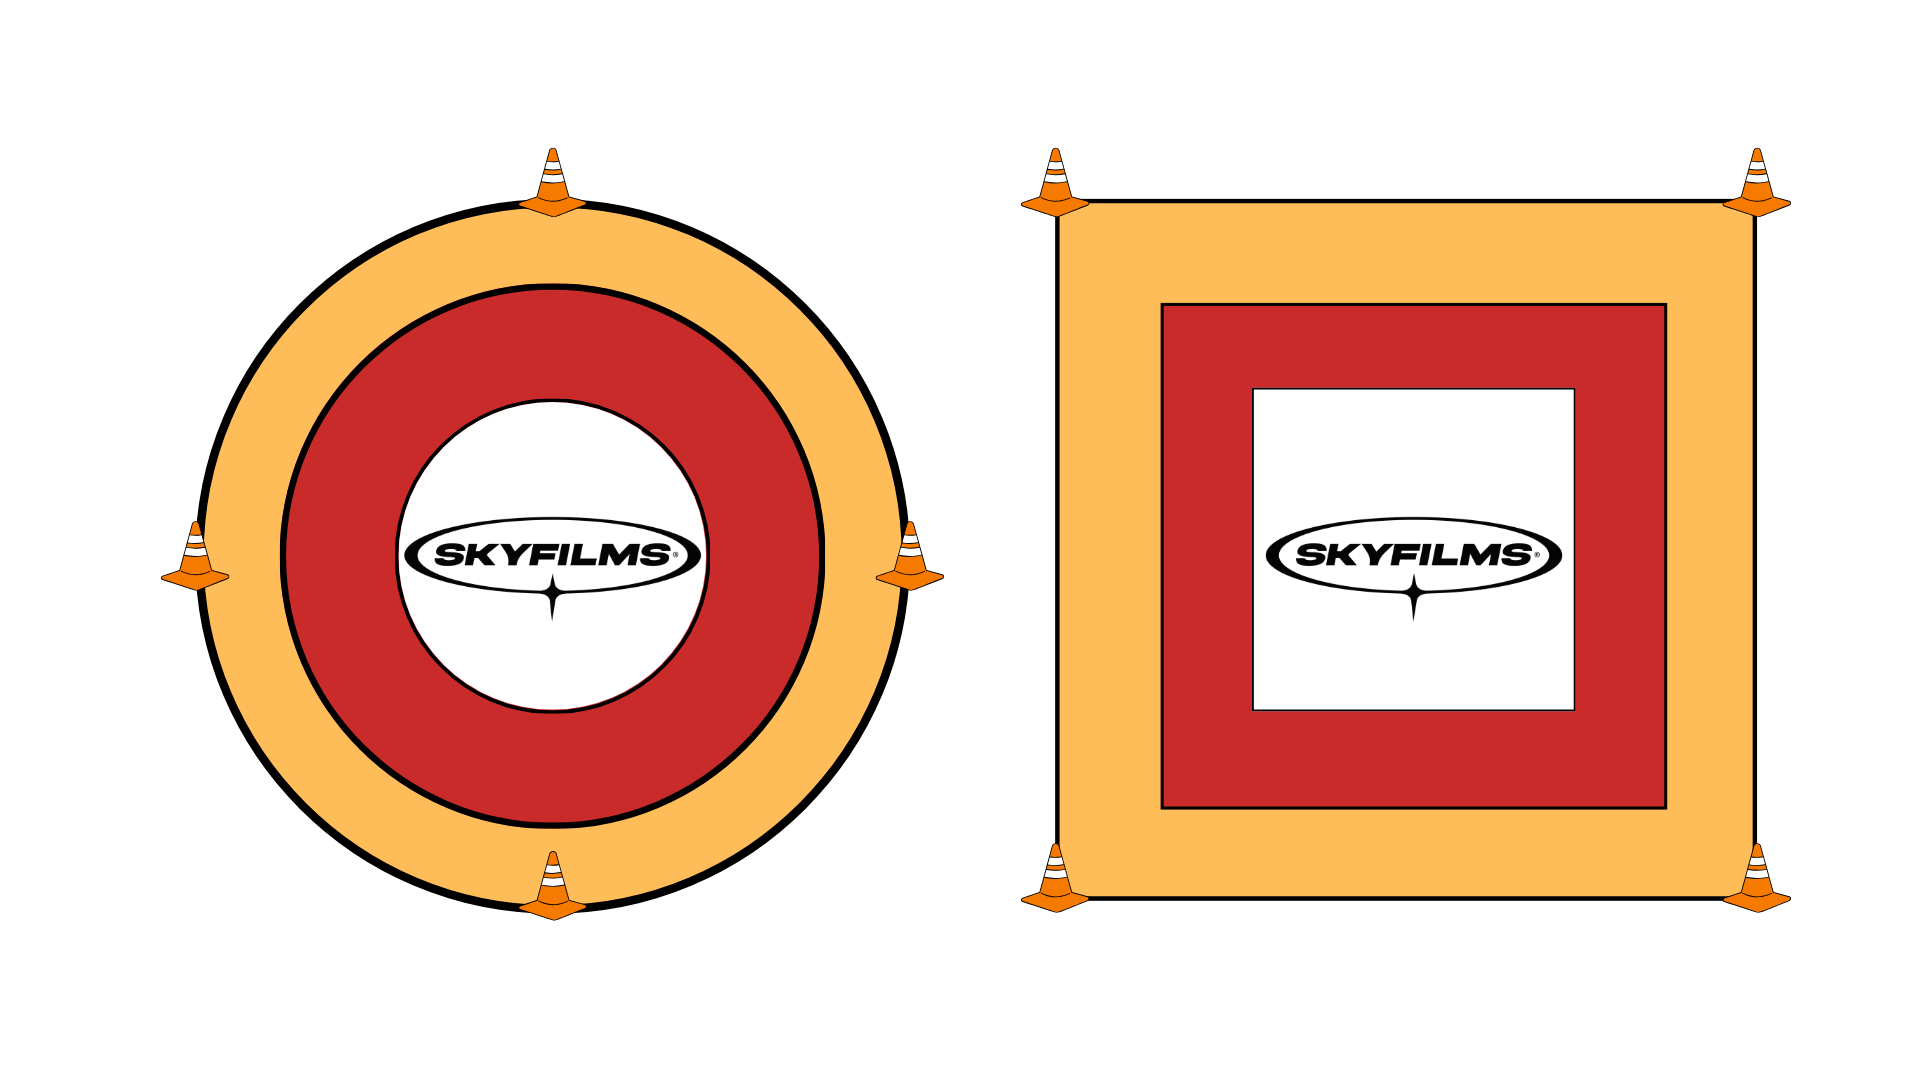
\includegraphics[width=.82\textwidth]{Imagenes/IMG_1597.PNG}
\caption{Ejemplo de delimitación física de un Área de Operación Temporal mediante conos y cinta de seguridad.}
\label{fig:delimitacion}
\end{figure}


\begin{figure}[H]
\centering
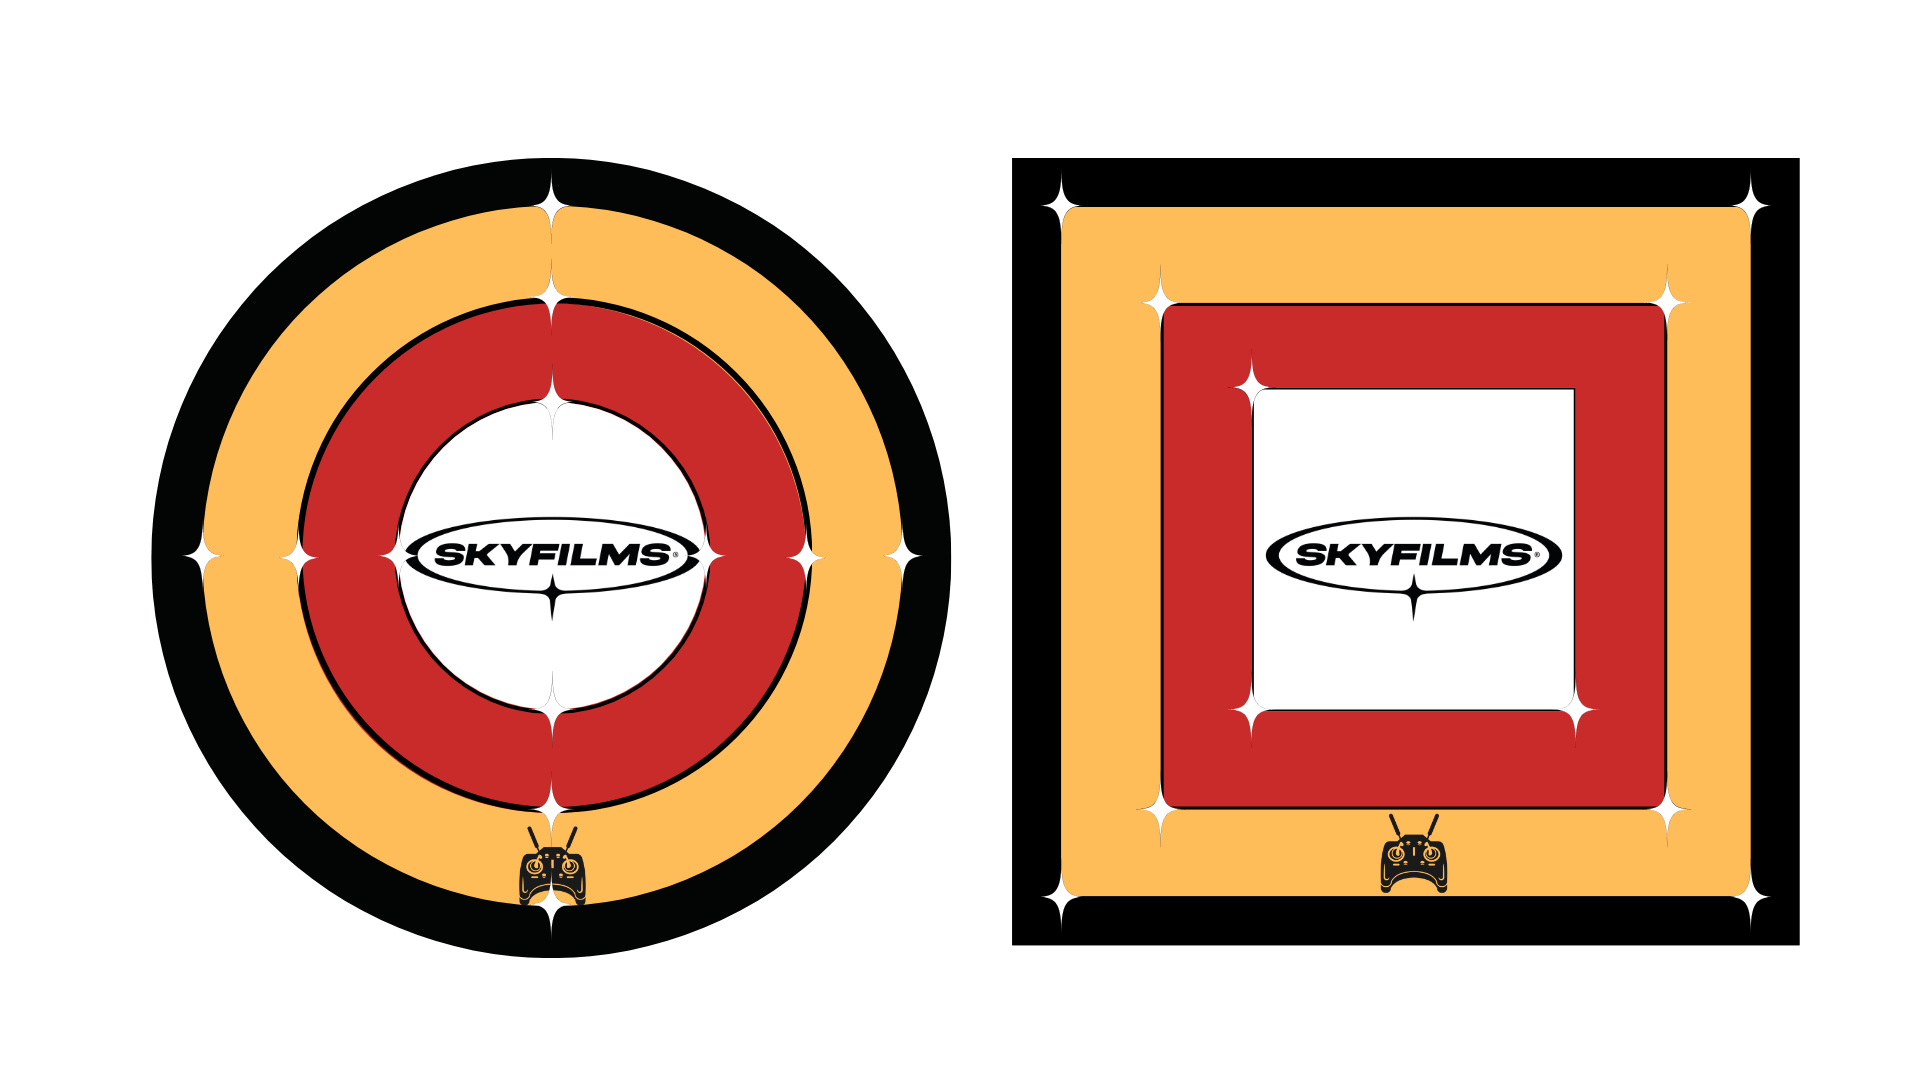
\includegraphics[width=.75\textwidth]{Imagenes/IMG_1596.PNG}
\caption{Ejemplo de iluminación portátil para operaciones en condiciones de baja iluminación.}
\label{fig:iluminacion}
\end{figure}


\begin{tcolorbox}[title=Documentos asociados,colback=gray!5,colframe=black]

\textbf{Procedimiento relacionado}

PO-001 – Planificación de la Operación

\vspace{0.3cm}

\textbf{Formatos relacionados}

\begin{itemize}

\item F-009 – Planificación de la Operación

\item F-011 – Evaluación del Riesgo Operacional

\item F-002 – Lista de Chequeo Preoperacional

\item F-010 – Briefing Operacional

\end{itemize}

\end{tcolorbox}







\subsection{Criterios para cancelar o reprogramar una operación}

Una operación deberá cancelarse, suspenderse o reprogramarse cuando se presente alguna de las siguientes condiciones:

\begin{itemize}

\item Condiciones meteorológicas incompatibles con una operación segura.

\item Restricciones del espacio aéreo que impidan la realización de la misión.

\item Fallas técnicas del UAS o de cualquiera de sus sistemas.

\item Indisponibilidad de personal competente.

\item Riesgos operacionales que superen el nivel aceptable definido por Skyfilms.

\item Ausencia de permisos o autorizaciones requeridas.

\item Cualquier otra condición que comprometa la seguridad operacional.

\end{itemize}

\begin{tcolorbox}[title=Documentos asociados,colback=gray!5,colframe=black]

\textbf{Procedimiento relacionado}

SOP-001 Planificación de la Operación.

\vspace{0.2cm}

\textbf{Formatos relacionados}

\begin{itemize}
\item F-008 Solicitud de Servicio.
\item F-009 Planificación de la Operación.
\item F-002 Lista de Chequeo Preoperacional.
\item F-001 Libro de Vuelo.
\end{itemize}

\end{tcolorbox}





\section{Evaluación del riesgo operacional}

Antes de la ejecución de cualquier operación UAS, Skyfilms S.A.S. realizará una evaluación del riesgo operacional con el fin de identificar los peligros asociados a la misión, analizar el nivel de riesgo y establecer las medidas de mitigación necesarias para garantizar un nivel de seguridad aceptable.

La evaluación del riesgo forma parte del proceso de planificación de la operación y constituye un requisito obligatorio antes de autorizar el inicio de cualquier misión.


\subsection{Objetivo}

La evaluación del riesgo operacional tiene como finalidad:

\begin{itemize}

\item Identificar peligros antes del inicio de la operación.

\item Analizar las amenazas presentes en el entorno operacional.

\item Definir medidas de mitigación.

\item Determinar la viabilidad operacional de la misión.

\item Proteger a las personas, bienes, espacio aéreo y aeronaves.

\end{itemize}

\subsection{Factores mínimos de evaluación}

\renewcommand{\arraystretch}{1.3}

\begin{longtable}{|p{5cm}|p{9cm}|}

\hline

\textbf{Factor} &
\textbf{Aspectos a evaluar}

\\ \hline

Espacio aéreo &
Clasificación, restricciones, NOTAM y proximidad a aeródromos.

\\ \hline

Meteorología &
Viento, lluvia, visibilidad, nubosidad y temperatura.

\\ \hline

Terreno &
Obstáculos, edificaciones, líneas eléctricas, cuerpos de agua y vegetación.

\\ \hline

Personas &
Presencia de terceros y control del área de operación.

\\ \hline

Infraestructura &
Edificaciones críticas, antenas, vías, puentes y otras estructuras.

\\ \hline

Tripulación &
Competencia, experiencia, estado físico y condición psicofísica.

\\ \hline

Aeronave &
Disponibilidad técnica, mantenimiento y estado general.

\\ \hline

Baterías &
Nivel de carga, ciclos, temperatura y estado físico.

\\ \hline

\end{longtable}

\subsection{Clasificación del riesgo}

Los riesgos identificados durante la planificación serán clasificados conforme a la metodología establecida en el Sistema de Gestión de la Seguridad Operacional (SMS).

Como criterio general, Skyfilms utilizará tres niveles de clasificación:

\begin{itemize}

\item Riesgo Bajo.

\item Riesgo Medio.

\item Riesgo Alto.

\end{itemize}

Las operaciones clasificadas como riesgo alto únicamente podrán ejecutarse cuando las medidas de mitigación implementadas permitan reducir el riesgo a un nivel aceptable.

\subsection{Medidas de mitigación}

Cuando durante la evaluación se identifique un riesgo operacional, podrán implementarse, entre otras, las siguientes medidas:

\begin{itemize}

\item Modificar el horario de la operación.

\item Cambiar el punto de despegue.

\item Reducir la altura de vuelo.

\item Delimitar el área de seguridad.

\item Incorporar un Observador Visual adicional.

\item Utilizar una aeronave diferente.

\item Posponer la misión.

\item Cancelar la operación.

\end{itemize}


\subsection{Aprobación}

La operación únicamente podrá iniciarse cuando la evaluación del riesgo haya sido completada y el nivel de riesgo residual resulte aceptable conforme a los criterios establecidos por Skyfilms.

Cuando el riesgo residual permanezca por encima del nivel aceptable, la misión deberá ser cancelada o reprogramada.



\begin{tcolorbox}[title=Documentos asociados,colback=gray!5,colframe=black]

\textbf{Procedimiento relacionado}

PO-002 Evaluación del Riesgo Operacional.

\vspace{0.2cm}

\textbf{Formatos relacionados}

\begin{itemize}

\item F-011 Evaluación del Riesgo Operacional.

\item F-009 Planificación de la Operación.

\item F-006 Reporte SMS (cuando aplique).

\end{itemize}

\end{tcolorbox}


\section{Briefing Operacional}

Antes del inicio de cualquier operación UAS, la tripulación deberá realizar un briefing operacional con el propósito de verificar que todas las condiciones técnicas, operacionales y de seguridad requeridas para la misión han sido comprendidas por el personal involucrado.

El briefing constituye la última verificación antes del inicio de la operación y permitirá confirmar que la planificación aprobada continúa siendo válida para las condiciones existentes en el lugar de la operación.

\subsection{Objetivos}

El briefing operacional tiene como objetivos:

\begin{itemize}

\item Confirmar el objetivo de la misión.

\item Asignar funciones y responsabilidades.

\item Revisar las condiciones meteorológicas reales.

\item Confirmar la disponibilidad técnica de la aeronave.

\item Revisar la evaluación del riesgo.

\item Verificar los procedimientos normales y de emergencia.

\item Resolver dudas antes del inicio de la operación.

\end{itemize}


\subsection{Participantes}

El briefing deberá realizarse con la participación de todo el personal involucrado en la operación, incluyendo, cuando aplique:

\begin{itemize}

\item Jefe de Pilotos.

\item Piloto Remoto.

\item Observador Visual.

\item Personal de apoyo.

\item Cliente o representante del cliente (cuando sea pertinente).

\end{itemize}

\subsection{Contenido mínimo}

\renewcommand{\arraystretch}{1.3}

\begin{longtable}{|p{5cm}|p{9cm}|}

\hline

\textbf{Tema} &
\textbf{Aspectos a revisar}

\\ \hline

Objetivo de la misión &
Alcance del servicio y producto esperado.

\\ \hline

Área de operación &
Zona de vuelo, límites, obstáculos y puntos de referencia.

\\ \hline

Meteorología &
Condiciones observadas antes del vuelo.

\\ \hline

Tripulación &
Asignación de funciones.

\\ \hline

Aeronave &
Estado técnico y configuración.

\\ \hline

Comunicaciones &
Canales de comunicación y palabras clave.

\\ \hline

Emergencias &
Procedimientos aplicables y puntos de reunión.

\\ \hline

Zonas de seguridad &
Despegue, aterrizaje y áreas restringidas.

\\ \hline

Terceros &
Control de acceso y protección de personas.

\\ \hline

\end{longtable}


\subsection{Confirmación de la tripulación}

Antes del inicio de la operación, el Piloto Remoto confirmará verbalmente que:

\begin{itemize}

\item La misión ha sido comprendida.

\item La aeronave se encuentra disponible para la operación.

\item Se conocen los procedimientos de emergencia.

\item No existen condiciones que impidan la ejecución segura de la misión.

\end{itemize}

El Observador Visual confirmará igualmente que comprende sus funciones y mantendrá comunicación permanente con el Piloto Remoto durante toda la operación.

\subsection{Modificaciones de última hora}

Cuando durante el briefing se identifiquen cambios significativos respecto a la planificación inicial, el Jefe de Pilotos deberá determinar si:

\begin{itemize}

\item La operación puede continuar sin modificaciones.

\item Es necesario actualizar la planificación.

\item Debe realizarse una nueva evaluación del riesgo.

\item La misión debe ser suspendida o reprogramada.

\end{itemize}


\begin{tcolorbox}[title=Documentos asociados,colback=gray!5,colframe=black]

\textbf{Procedimiento relacionado}

PO-003 Briefing Operacional.

\vspace{0.2cm}

\textbf{Formatos relacionados}

\begin{itemize}

\item F-010 Briefing Operacional.

\item F-009 Planificación de la Operación.

\item F-011 Evaluación del Riesgo Operacional.

\item F-002 Lista de Chequeo Preoperacional.

\end{itemize}

\end{tcolorbox}

\section{Ejecución de la Operación}

La ejecución de una operación UAS comprende el conjunto de actividades desarrolladas desde el inicio de la inspección preoperacional hasta la finalización del vuelo y aseguramiento de la aeronave.

Todas las operaciones deberán ejecutarse conforme a la planificación aprobada, la evaluación del riesgo realizada, las limitaciones establecidas en las OpSpecs y los procedimientos definidos en el presente Manual de Operaciones.









\subsection{Inspección preoperacional}

Antes de cada vuelo, el Piloto Remoto deberá realizar una inspección preoperacional de la aeronave y de todos los equipos asociados.

La inspección tendrá como finalidad verificar que la aeronave se encuentra en condiciones técnicas adecuadas para la operación y que no existen condiciones que comprometan la seguridad del vuelo.

La inspección deberá quedar registrada mediante la Lista de Chequeo Preoperacional correspondiente.


\subsubsection*{Aspectos mínimos a verificar}

\begin{itemize}

\item Estado general de la aeronave.

\item Integridad estructural.

\item Hélices correctamente instaladas.

\item Estado de motores.

\item Nivel de carga de baterías.

\item Estado del control remoto.

\item Sistema de navegación.

\item Sistema de posicionamiento.

\item Tarjeta de memoria.

\item Configuración de Return To Home (RTH).

\item Espacio aéreo habilitado.

\item Área libre para despegue y aterrizaje.

\end{itemize}


\subsection{Inicio de la operación}

Antes del despegue, el Piloto Remoto verificará que:

\begin{itemize}

\item El briefing haya finalizado.

\item La evaluación del riesgo se encuentre aprobada.

\item No existan cambios significativos en las condiciones meteorológicas.

\item El área de operación permanezca controlada.

\item El Observador Visual se encuentre en posición.

\item La aeronave disponga de suficiente autonomía para cumplir la misión.

\end{itemize}

Únicamente cuando todas estas condiciones hayan sido verificadas podrá iniciarse el vuelo.


\subsection{Desarrollo del vuelo}

Durante la ejecución de la misión, el Piloto Remoto deberá:

\begin{enumerate}

\item Mantener el control de la aeronave en todo momento.

\item Operar dentro de las limitaciones autorizadas.

\item Supervisar permanentemente el estado del UAS.

\item Mantener comunicación con el Observador Visual cuando aplique.

\item Monitorear continuamente el entorno operacional.

\item Interrumpir inmediatamente la operación cuando se identifique una condición insegura.

\end{enumerate}

\subsection{Funciones del Observador Visual durante la operación}

Cuando la operación requiera Observador Visual, este deberá:

\begin{itemize}

\item Mantener contacto visual permanente con la aeronave.

\item Informar oportunamente cualquier riesgo.

\item Vigilar la presencia de terceros.

\item Alertar sobre otras aeronaves.

\item Supervisar el área de seguridad.

\item Apoyar la aplicación de procedimientos de emergencia.

\end{itemize}


\subsection{Suspensión inmediata de la operación}

El Piloto Remoto deberá suspender inmediatamente la operación cuando ocurra cualquiera de las siguientes situaciones:

\begin{itemize}

\item Pérdida de control de la aeronave.

\item Aparición de aeronaves tripuladas.

\item Ingreso de personas al área crítica de operación.

\item Condiciones meteorológicas adversas.

\item Advertencias críticas del sistema.

\item Disminución del nivel de batería por debajo de los límites establecidos.

\item Cualquier condición que comprometa la seguridad operacional.

\end{itemize}

\subsection{Finalización del vuelo}

Una vez concluida la misión, el Piloto Remoto deberá:

\begin{enumerate}

\item Aterrizar en la zona prevista.

\item Apagar la aeronave.

\item Asegurar las baterías.

\item Realizar una inspección visual posterior al vuelo.

\item Informar cualquier novedad presentada durante la operación.

\item Registrar la información correspondiente en el Libro de Vuelo.

\end{enumerate}

\begin{tcolorbox}[title=Documentos asociados,colback=gray!5,colframe=black]

\textbf{Procedimiento relacionado}

PO-004 Ejecución de la Operación.

\vspace{0.3cm}

\textbf{Formatos relacionados}

\begin{itemize}

\item F-001 Libro de Vuelo.

\item F-002 Lista de Chequeo Preoperacional.

\item F-003 Lista de Chequeo Postoperacional.

\item F-009 Planificación de la Operación.

\item F-010 Briefing Operacional.

\item F-011 Evaluación del Riesgo Operacional.

\end{itemize}

\end{tcolorbox}

\section{Gestión del Enlace (C2)}

El enlace de Mando y Control (Command and Control - C2) constituye el medio principal de comunicación entre la estación de control en tierra y la aeronave no tripulada, permitiendo la transmisión de comandos, telemetría y demás información necesaria para el desarrollo seguro de la operación.

Durante todas las fases del vuelo, el Piloto Remoto será responsable de supervisar permanentemente la calidad del enlace C2 y de adoptar las acciones necesarias cuando se presenten degradaciones o pérdidas del mismo.

Skyfilms utilizará sistemas de enlace C2 certificados por los fabricantes de las aeronaves empleadas, configurados conforme a las recomendaciones técnicas y a las limitaciones establecidas por la normativa aplicable.


\subsection{Supervisión del enlace C2}

Antes y durante cada operación, el Piloto Remoto deberá verificar continuamente el estado del enlace C2 mediante los indicadores disponibles en la estación de control.

Como mínimo deberán supervisarse los siguientes parámetros:

\renewcommand{\arraystretch}{1.3}

\begin{longtable}{|p{4.5cm}|p{4cm}|p{4cm}|}
\hline

\textbf{Parámetro} &
\textbf{DJI Mavic 4 Pro} &
\textbf{Pavo20 Pro}

\\ \hline

Calidad del enlace &
Indicador de señal &
RSSI / LQ

\\ \hline

Telemetría &
Disponible &
Disponible

\\ \hline

Alertas visuales &
Sí &
Sí

\\ \hline

Alertas sonoras &
Sí &
Sí

\\ \hline

Estado del enlace &
En tiempo real &
En tiempo real

\\ \hline

\end{longtable}



\subsection{Gestión de la degradación del enlace}

Cuando durante la operación se detecte una disminución en la calidad del enlace C2, el Piloto Remoto deberá adoptar, según corresponda, las siguientes acciones:

\begin{itemize}

\item Reducir la distancia respecto a la aeronave.

\item Disminuir la altura de operación cuando resulte conveniente.

\item Reorientar las antenas del sistema de control.

\item Evitar obstáculos que puedan afectar la propagación de la señal.

\item Mantener comunicación permanente con el Observador Visual.

\item Prepararse para finalizar la misión si la condición persiste.

\end{itemize}

\begin{figure}[H]
\centering
\begin{tikzpicture}[
font=\small,
node distance=7mm,
box/.style={
rectangle,
rounded corners,
draw,
align=center,
minimum width=4.5cm,
minimum height=0.9cm
},
arrow/.style={
-{Latex},
thick
}
]

\node[box] (a) {Operación normal};

\node[box, below=of a] (b) {Degradación del enlace C2};

\node[box, below=of b] (c) {Aplicar medidas correctivas};

\node[box, below=of c] (d) {¿Se recupera el enlace?};

\node[box, below left=1cm and 1.8cm of d] (e) {Continuar la operación};

\node[box, below right=1cm and 1.8cm of d] (f) {Activar procedimiento de pérdida del enlace};

\node[box, below=of f] (g) {RTH / LAND / Failsafe};

\node[box, below=of g] (h) {Registrar evento e informar al SMS};

\draw[arrow] (a)--(b);
\draw[arrow] (b)--(c);
\draw[arrow] (c)--(d);

\draw[arrow] (d)--node[left]{Sí}(e);
\draw[arrow] (d)--node[right]{No}(f);

\draw[arrow] (f)--(g);
\draw[arrow] (g)--(h);

\end{tikzpicture}

\caption{Gestión general de la degradación del enlace C2.}
\end{figure}


\subsection{Pérdida del enlace C2}

Cuando se presente una pérdida total del enlace de mando y control, la tripulación deberá aplicar los procedimientos automáticos y operacionales definidos para cada tipo de aeronave.

\renewcommand{\arraystretch}{1.3}

\begin{longtable}{|p{4.5cm}|p{6cm}|p{3cm}|}

\hline

\textbf{Sistema} &
\textbf{Acción inmediata} &
\textbf{Continuidad}

\\ \hline

DJI Mavic 4 Pro &
Permitir la activación automática del Return To Home (RTH) o del procedimiento configurado para pérdida de enlace. &
Cancelar la misión.

\\ \hline

Pavo20 Pro &
Permitir la ejecución del Failsafe configurado (RTH, LAND o procedimiento autorizado). &
Cancelar la misión.

\\ \hline

\end{longtable}


\subsection{Gestión de interferencias}

Cuando se identifique una posible interferencia electromagnética que afecte el enlace C2, el Piloto Remoto deberá:

\begin{itemize}

\item Identificar el origen probable de la interferencia.

\item Modificar la posición de operación cuando sea posible.

\item Evitar la proximidad a fuentes conocidas de interferencia.

\item Suspender la operación cuando no sea posible garantizar un enlace seguro.

\end{itemize}

Las interferencias podrán originarse por:

\begin{itemize}

\item Redes Wi-Fi.

\item Infraestructura de telecomunicaciones.

\item Equipos industriales.

\item Condiciones atmosféricas.

\item Obstáculos físicos.

\end{itemize}


\subsection{Limitaciones operacionales}

La confiabilidad del enlace C2 dependerá de factores propios del entorno operacional y de las características técnicas del sistema empleado.

Durante las operaciones deberán considerarse, entre otras, las siguientes limitaciones:

\begin{itemize}

\item Obstáculos naturales o artificiales.

\item Condiciones meteorológicas adversas.

\item Interferencias electromagnéticas.

\item Tipo de operación autorizada (VLOS).

\item Distancia entre la estación de control y la aeronave.

\end{itemize}

\subsection{Referencias técnicas}

Las especificaciones técnicas particulares de cada sistema de enlace C2, incluyendo frecuencias de operación, protocolos de comunicación, configuraciones de \textit{failsafe}, firmware, equipos compatibles y demás características técnicas, se encuentran documentadas en las Fichas Técnicas de Aeronave (FTA) y en el Manual de Control de Mantenimiento (MCM), documentos controlados por Skyfilms S.A.S.

Las FTA forman parte del Sistema de Gestión Documental de la organización y deberán mantenerse actualizadas conforme a las configuraciones aprobadas para cada aeronave.

\begin{tcolorbox}[
title=Nota Operacional,
colback=blue!5,
colframe=blue!60!black]

El Piloto Remoto deberá considerar cualquier degradación del enlace C2 como una condición potencialmente insegura. Si las medidas de mitigación no restablecen un nivel aceptable de confiabilidad del enlace, la misión deberá finalizar de manera controlada y el evento será registrado conforme a los procedimientos del Sistema de Gestión de la Seguridad Operacional (SMS).

\end{tcolorbox}










\section{Procedimientos especiales de operación}

Determinadas operaciones desarrolladas por Skyfilms requieren la adopción de medidas adicionales de planificación, coordinación y control debido a las características particulares del entorno operacional o del tipo de misión.

Los procedimientos descritos en esta sección complementan los procedimientos generales establecidos en el presente Manual de Operaciones y deberán aplicarse cuando corresponda.


\subsection{Operaciones FPV}

Las operaciones mediante aeronaves FPV (\textit{First Person View}) estarán destinadas a la obtención de secuencias audiovisuales dinámicas y se ejecutarán estrictamente bajo condiciones de Visibilidad en Línea de Vista (VLOS), conforme a lo establecido en el RAC 100.

Dado que el Piloto Remoto utiliza un dispositivo de visión en primera persona (gafas/visor) que limita su percepción visual del entorno circundante, es de carácter \textbf{obligatorio} el cumplimiento de las siguientes directrices operacionales para mitigar el riesgo:

\begin{itemize}
    \item \textbf{Observador Visual Dedicado:} Toda operación FPV debe contar obligatoriamente con la presencia ininterrumpida de al menos un Observador Visual.
    \item \textbf{Contacto Visual Directo (VLOS):} El Observador Visual será el responsable de mantener el contacto visual directo y constante con la aeronave (UA) y su entorno en todo momento, sin el uso de ayudas ópticas o electrónicas (diferentes a lentes correctivos).
    \item \textbf{Comunicación Efectiva:} Debe existir una comunicación verbal clara, constante y en tiempo real entre el Piloto Remoto y el Observador Visual para alertar sobre obstáculos, tráfico aéreo tripulado o incursiones de terceros.
    \item \textbf{Límites del Área de Operación:} El área de vuelo debe ser evaluada previamente para garantizar que la aeronave nunca exceda el radio visual del Observador (límite máximo legal de 750 metros horizontales).
\end{itemize}<


\subsection{Operaciones en zonas urbanas}

Antes de operar en entornos urbanos deberá verificarse:

\begin{itemize}

\item Presencia de terceros.

\item Obstáculos verticales.

\item Interferencias electromagnéticas.

\item Disponibilidad de zonas de aterrizaje de emergencia.

\item Control del perímetro operacional.

\end{itemize}

\subsection{Operaciones cerca de infraestructura}

Cuando la operación se realice en proximidad de edificaciones, puentes, torres, antenas u otras estructuras, el Piloto Remoto deberá:

\begin{enumerate}

\item Mantener una distancia de seguridad.

\item Identificar posibles efectos de turbulencia.

\item Verificar la recepción GNSS.

\item Mantener rutas de escape previamente definidas.

\end{enumerate}


\subsection{Operaciones en eventos}

Las operaciones destinadas al cubrimiento de eventos deberán considerar, como mínimo:

\begin{itemize}

\item Control del público.

\item Coordinación con el organizador.

\item Delimitación del área de operación.

\item Identificación de rutas de evacuación.

\item Procedimientos para suspensión inmediata del vuelo.

\end{itemize}

Cuando la operación implique concentraciones de personas, únicamente podrá desarrollarse si cuenta con las autorizaciones exigidas por la Aeronáutica Civil y se han implementado las medidas de mitigación correspondientes.



\subsection{Operaciones en zonas rurales}

Durante operaciones en áreas rurales deberán evaluarse, entre otros:

\begin{itemize}

\item Líneas eléctricas.

\item Árboles.

\item Animales.

\item Condiciones del terreno.

\item Cobertura de comunicaciones.

\end{itemize}


\subsection{Operaciones cerca de cuerpos de agua}

Cuando la misión se desarrolle sobre o cerca de cuerpos de agua, deberán adoptarse medidas adicionales para:

\begin{itemize}

\item Identificar zonas seguras de aterrizaje.

\item Evitar pérdida de referencia visual.

\item Considerar efectos del viento.

\item Establecer procedimientos ante amerizaje accidental.

\end{itemize}


\subsection{Vuelo Nocturno}

Skyfilms S.A.S. ejecutará operaciones de vuelo nocturno para la captura de material audiovisual cinematográfico y comercial, dando estricto cumplimiento a las exigencias operacionales y de seguridad establecidas por la Aerocivil para la Categoría Específica.

Para la ejecución y autorización de vuelos nocturnos, el Piloto Remoto y el equipo operativo deberán verificar y cumplir ineludiblemente con los siguientes requisitos previos y durante el vuelo:

\begin{itemize}
    \item \textbf{Adición en el Certificado:} El Piloto Remoto al mando debe contar de manera obligatoria con la adición vigente de ``Vuelo Nocturno'' en su Certificado de Idoneidad como piloto UAS (CIPU).
    \item \textbf{Iluminación de la Aeronave:} La aeronave no tripulada (UA) debe operar con las luces instaladas de fábrica o autorizadas por su fabricante, encendidas de forma permanente durante toda la operación nocturna (RAC 100.220 a). Estas luces deben hacer a la aeronave claramente visible en el cielo nocturno para la tripulación y para otras aeronaves en el espacio aéreo. En el DJI Mavic 4 Pro, los ledes delanteros se configuran para permanecer encendidos; el modo \textit{Auto} los apaga al grabar y no debe usarse de noche. Antes de cada vuelo se verifica que las luces funcionan, y no se instalan accesorios que no estén autorizados por el fabricante.
    \item \textbf{Modalidad de Vuelo Estricta:} La operación nocturna se restringirá \textbf{únicamente a la modalidad VLOS} (Visibilidad en Línea de Vista), sin exceder en ningún momento un radio de 750 metros horizontales medidos desde la posición fija del piloto.
    \item \textbf{Reconocimiento Diurno Obligatorio (Scouting):} Es de carácter mandatorio realizar una inspección física y visual del área de operación en horario diurno (con luz solar) antes de la ejecución del vuelo nocturno en esa misma locación. Este reconocimiento tiene como objetivo principal la identificación de obstáculos no iluminados (líneas eléctricas, cables, antenas, vegetación alta) y el establecimiento de rutas de vuelo seguras y puntos de aterrizaje de emergencia.
    \item \textbf{Apoyo de Observador Visual:} Toda operación nocturna requerirá incondicionalmente el apoyo de un Observador Visual asignado por el Jefe de Pilotos, quien asistirá en el monitoreo del entorno para prevenir colisiones e identificar cualquier amenaza en la oscuridad.
    \item \textbf{Límites de la operación:} el tiempo de vuelo planificado no excederá el 80\,\% de la autonomía de la aeronave (RAC 100.210 k); la operación se realiza desde un punto fijo (RAC 100.210 n) y a una altura máxima de 400 ft (122 m) sobre el terreno. En zona urbana se mantiene una distancia mínima de 30 m a personas y edificaciones (RAC 100.220 b).
    \item \textbf{Falla de iluminación:} si las luces de la aeronave se apagan o fallan durante el vuelo, el Piloto Remoto aterriza de inmediato en el punto seguro más cercano e informa al Observador Visual y al Jefe de Pilotos.
    \item \textbf{Lista de chequeo y riesgo nocturno:} toda operación nocturna incluye la sección nocturna de la Lista de Chequeo Preoperacional (F-002) y una Evaluación del Riesgo Operacional (F-011) que considere la pérdida de referencias visuales, la desorientación espacial y los obstáculos no iluminados.
\end{itemize}

\section{Procedimientos Anormales y de Emergencia}

Skyfilms S.A.S. establece procedimientos estandarizados para responder de manera rápida, segura y coordinada ante condiciones anormales o situaciones de emergencia que puedan presentarse durante las operaciones UAS.

El objetivo de estos procedimientos es proteger la vida e integridad de las personas, preservar la seguridad del espacio aéreo, minimizar daños materiales y garantizar la adecuada gestión posterior del evento.


\subsection{Generalidades}

Ante cualquier condición anormal o emergencia, el Piloto Remoto deberá aplicar los siguientes principios:

\begin{enumerate}

\item Mantener la calma.

\item Priorizar la seguridad de las personas.

\item Mantener el control de la aeronave cuando sea posible.

\item Aplicar el procedimiento correspondiente.

\item Informar inmediatamente al Observador Visual.

\item Suspender la operación cuando la seguridad operacional se vea comprometida.

\item Reportar el evento conforme al Sistema de Gestión de la Seguridad Operacional (SMS).

\end{enumerate}

\subsection{Clasificación de condiciones anormales y emergencias}

Las situaciones que puedan presentarse durante una operación UAS se clasifican en las siguientes categorías:

\begin{enumerate}[label=\Alph*.]

\item Condiciones Anormales

\item Emergencias Técnicas

\item Emergencias Operacionales

\item Emergencias Ambientales

\item Emergencias Médicas

\item Accidentes

\end{enumerate}


\subsection{Condiciones Anormales}

Se consideran condiciones anormales aquellas situaciones que afectan el desarrollo de la misión, pero que permiten mantener el control de la aeronave y finalizar la operación de manera segura mediante la aplicación de los procedimientos establecidos.

\renewcommand{\arraystretch}{1.4}

\begin{longtable}{|p{4.5cm}|p{6cm}|p{3.5cm}|}
\hline

\textbf{Condición} &
\textbf{Acción inmediata} &
\textbf{Continuidad}

\\ \hline

Incremento del viento &
Evaluar la estabilidad del vuelo y considerar el retorno al punto de aterrizaje. &
Continuar únicamente si el riesgo permanece aceptable.

\\ \hline

Disminución de señal GNSS &
Mantener el control manual, evitar maniobras críticas y monitorear la estabilidad de la aeronave. &
Reevaluar la misión.

\\ \hline

Consumo elevado de batería &
Reducir la duración de la misión y regresar de inmediato al punto de aterrizaje. &
Finalizar la operación.

\\ \hline

Pérdida temporal del video FPV &
Mantener comunicación con el Observador Visual y recuperar el enlace de video. &
Continuar únicamente si el enlace se restablece completamente.

\\ \hline

\end{longtable}




\subsection{Emergencias Técnicas}

Las emergencias técnicas corresponden a fallas del sistema UAS que pueden comprometer la seguridad de la operación y requieren una respuesta inmediata.

\renewcommand{\arraystretch}{1.4}

\begin{longtable}{|p{4.5cm}|p{6cm}|p{3.5cm}|}
\hline

\textbf{Emergencia} &
\textbf{Acción inmediata} &
\textbf{Continuidad}

\\ \hline

Pérdida del enlace C2 &
Esperar la recuperación automática del enlace o la activación del Return To Home (RTH). &
Cancelar la misión.

\\ \hline

Fly Away &
Intentar recuperar el control, alertar al Observador Visual y proteger a terceros. &
Operación suspendida.

\\ \hline

Falla de motor &
Realizar aterrizaje inmediato en una zona segura. &
Operación suspendida.

\\ \hline

Falla de hélice &
Reducir riesgos para terceros y aterrizar inmediatamente. &
Operación suspendida.

\\ \hline

Error crítico del sistema &
Suspender la operación y asegurar la aeronave. &
Operación suspendida.

\\ \hline

\end{longtable}


\subsection{Emergencias Operacionales}

Las emergencias operacionales corresponden a situaciones originadas por factores externos durante el desarrollo de la misión.

\renewcommand{\arraystretch}{1.4}

\begin{longtable}{|p{4.5cm}|p{6cm}|p{3.5cm}|}
\hline

\textbf{Emergencia} &
\textbf{Acción inmediata} &
\textbf{Continuidad}

\\ \hline

Ingreso de personas al área &
Suspender temporalmente la operación y mantener la aeronave en condición segura o aterrizar si es necesario. &
Continuar únicamente cuando el área vuelva a estar controlada.

\\ \hline

Presencia de aeronave tripulada &
Descender inmediatamente o aterrizar, manteniendo separación segura. &
Reanudar únicamente cuando desaparezca el conflicto.

\\ \hline

Pérdida del Observador Visual &
Suspender inmediatamente la misión FPV y aterrizar la aeronave. &
Operación suspendida.

\\ \hline

Interferencia operacional &
Alejar la aeronave y reevaluar el escenario operacional. &
Continuar únicamente si desaparece la condición de riesgo.

\\ \hline

\end{longtable}

\subsection{Emergencias Ambientales}

Las emergencias ambientales corresponden a cambios inesperados en las condiciones del entorno.

\renewcommand{\arraystretch}{1.4}

\begin{longtable}{|p{4.5cm}|p{6cm}|p{3.5cm}|}
\hline

\textbf{Emergencia} &
\textbf{Acción inmediata} &
\textbf{Continuidad}

\\ \hline

Lluvia &
Aterrizar inmediatamente. &
Cancelar la misión.

\\ \hline

Tormenta eléctrica &
Cancelar inmediatamente la operación y asegurar los equipos. &
Operación suspendida.

\\ \hline

Incremento súbito del viento &
Regresar al punto de aterrizaje. &
Reevaluar condiciones antes de continuar.

\\ \hline

Humo o incendio cercano &
Alejar la aeronave y abandonar el área afectada. &
Operación suspendida.

\\ \hline

Reducción significativa de la visibilidad &
Aterrizar tan pronto como sea seguro hacerlo. &
Cancelar la misión.

\\ \hline

\end{longtable}

\subsection{Emergencias Médicas}

Cuando durante una operación se presente una emergencia médica deberán aplicarse las siguientes acciones iniciales.

\renewcommand{\arraystretch}{1.4}

\begin{longtable}{|p{4.5cm}|p{6cm}|p{3.5cm}|}
\hline

\textbf{Emergencia} &
\textbf{Acción inmediata} &
\textbf{Continuidad}

\\ \hline

Lesión leve &
Aplicar primeros auxilios y evaluar la condición del afectado. &
Continuar únicamente si no existe afectación para la seguridad.

\\ \hline

Lesión grave &
Activar el Sistema de Emergencias Médicas (SEM) y suspender la operación. &
Operación suspendida.

\\ \hline

Incapacidad del Piloto Remoto &
Asegurar la aeronave y solicitar asistencia médica. &
Operación suspendida.

\\ \hline

Emergencia médica de un tercero &
Priorizar la atención del afectado y coordinar con los servicios de emergencia. &
Operación suspendida hasta garantizar condiciones seguras.

\\ \hline

\end{longtable}




\subsection{Accidentes}

Cuando ocurra un accidente durante una operación UAS, la tripulación deberá:

\begin{enumerate}

\item Priorizar la atención de personas lesionadas.

\item Asegurar el área de operación.

\item Evitar modificar la escena del evento salvo que exista riesgo adicional.

\item Informar al Jefe de Pilotos.

\item Informar al Gerente SMS.

\item Preservar la evidencia disponible.

\item Elaborar el reporte correspondiente conforme al SMS.

\end{enumerate}


\begin{tcolorbox}[title=Documentos asociados,colback=gray!5,colframe=black]

\textbf{Procedimiento relacionado}

PO-005 Gestión de Condiciones Anormales y Emergencias.

\vspace{0.3cm}

\textbf{Formatos relacionados}

\begin{itemize}

\item F-006 Reporte SMS.

\item F-012 Reporte de Peligros.

\item F-013 Reporte de Incidente o Accidente.

\item F-001 Libro de Vuelo.

\end{itemize}

\end{tcolorbox}


\section{Finalización de la Operación}

La finalización de una operación comprende todas las actividades posteriores al aterrizaje de la aeronave, orientadas a garantizar el cierre seguro de la misión, la preservación de los equipos, la actualización de los registros operacionales y la disponibilidad de la aeronave para futuras operaciones.

Ninguna misión se considerará finalizada hasta completar la totalidad de las actividades de cierre descritas en el presente procedimiento.

\subsection{Aseguramiento de la aeronave}

Una vez concluido el vuelo, el Piloto Remoto deberá:

\begin{enumerate}

\item Apagar la aeronave.

\item Apagar el control remoto.

\item Retirar la batería.

\item Verificar la temperatura de las baterías.

\item Realizar una inspección visual del UAS.

\item Asegurar todos los equipos antes del transporte.

\end{enumerate}


\subsection{Inspección postoperacional}

Después de cada operación deberá realizarse una inspección visual de la aeronave con el propósito de identificar daños, desgaste o cualquier condición que pueda afectar la aeronavegabilidad del UAS.

Como mínimo deberán verificarse:

\begin{itemize}

\item Estado estructural.

\item Hélices.

\item Motores.

\item Cámara.

\item Gimbal.

\item Baterías.

\item Antenas.

\item Tornillería visible.

\item Estado general de limpieza.

\end{itemize}


\subsection{Gestión de baterías}

Finalizada la operación, las baterías deberán:

\begin{itemize}

\item Registrarse en el control de baterías.

\item Verificarse visualmente.

\item Almacenarse conforme a las recomendaciones del fabricante.

\item Retirarse del servicio cuando presenten daños o comportamientos anormales.

\end{itemize}

\subsection{Gestión del material capturado}

Terminada la operación, el material audiovisual deberá descargarse, verificarse y almacenarse conforme al procedimiento interno de gestión de la información.

La descarga del material deberá realizarse antes de reutilizar las tarjetas de memoria empleadas durante la misión.


\subsection{Debriefing operacional}

Cuando la complejidad de la misión lo amerite, la tripulación realizará un debriefing con el propósito de:

\begin{itemize}

\item Analizar el desarrollo de la operación.

\item Identificar oportunidades de mejora.

\item Registrar novedades.

\item Identificar peligros observados.

\item Retroalimentar futuros procedimientos.

\end{itemize}

\subsection{Cierre operacional}

Antes de dar por finalizada la misión deberá verificarse que:

\begin{itemize}

\item Se diligenció el Libro de Vuelo.

\item Se diligenciaron los formatos aplicables.

\item No existen novedades pendientes.

\item La aeronave quedó disponible para una nueva operación o fue remitida a mantenimiento.

\item Los reportes SMS fueron realizados cuando corresponda.

\end{itemize}


\begin{tcolorbox}[title=Documentos asociados,colback=gray!5,colframe=black]

\textbf{Procedimiento relacionado}

PO-006 Finalización de la Operación.

\vspace{0.3cm}

\textbf{Formatos relacionados}

\begin{itemize}

\item F-001 Libro de Vuelo.

\item F-003 Lista de Chequeo Postoperacional.

\item F-004 Registro de Baterías.

\item F-006 Reporte SMS.

\item F-013 Reporte de Incidente o Accidente (cuando aplique).

\end{itemize}

\end{tcolorbox}



\section{Manejo y Transporte de Mercancías Peligrosas (Baterías UAS)}

Aunque Skyfilms S.A.S. excluye el transporte comercial de mercancías peligrosas como carga útil, reconoce que las baterías de Litio-Polímero (LiPo) y Iones de Litio (Li-ion) utilizadas para propulsar las aeronaves (Mavic 4 Pro y FPV) y equipos de estación de tierra, son clasificadas legalmente como Mercancías Peligrosas (Clase 9 - Varios) bajo la normativa aeronáutica internacional y nacional.

Para garantizar la seguridad operacional, el personal deberá cumplir estrictamente el siguiente procedimiento para el control, manejo, transporte, almacenamiento y disposición final de las baterías:

\begin{enumerate}
    \item \textbf{Transporte Terrestre y Aéreo:}
    \begin{itemize}
        \item Las baterías nunca deben transportarse instaladas en la aeronave.
        \item Deben transportarse descargadas a un nivel de almacenamiento seguro (entre 30\% y 50\% de su capacidad).
        \item Es obligatorio el uso de bolsas ignífugas (\textit{LiPo Safe Bags}) o estuches rígidos individuales que aíslen los terminales para prevenir cortocircuitos.
        \item En caso de desplazamiento en vuelos comerciales (aerolíneas), las baterías deben llevarse exclusivamente en el equipaje de mano, con los terminales aislados con cinta no conductiva, cumpliendo los límites de Watt-hora (Wh) de la IATA.
    \end{itemize}

    \item \textbf{Carga y Descarga en Locación:}
    \begin{itemize}
        \item La carga de baterías en campo se realizará exclusivamente en áreas ventiladas, alejadas de materiales inflamables y exposición directa al sol.
        \item El Piloto nunca dejará desatendido un proceso de carga.
        \item Si una batería presenta un incremento inusual de temperatura durante la carga, el proceso se interrumpirá inmediatamente y se aislará la batería.
    \end{itemize}

    \item \textbf{Almacenamiento y Mantenimiento:}
    \begin{itemize}
        \item Las baterías se almacenarán en la base principal en gabinetes ventilados a temperatura ambiente (15°C a 25°C).
        \item Se debe inspeccionar visualmente cada batería antes de su uso para descartar hinchamiento (\textit{puffing}), perforaciones, o cables expuestos. Una batería con cualquiera de estas condiciones se declarará inoperativa.
    \end{itemize}

    \item \textbf{Disposición Final:}
    \begin{itemize}
        \item Las baterías declaradas inoperativas o que hayan cumplido su ciclo de vida útil (aprox. 200 ciclos) no serán desechadas en la basura común.
        \item Serán descargadas completamente (0V) mediante un descargador resistivo o sumergidas en solución salina (protocolo LiPo), y posteriormente entregadas a un gestor ambiental certificado para el manejo de Residuos de Aparatos Eléctricos y Electrónicos (RAEE).
    \end{itemize}
\end{enumerate}

















% Fin del Capítulo 3




\label{fin_cap3} %

% Capítulo 4: Entrenamiento del Personal UAS

\chapter{Personal UAS}
\label{chap:04_personal}

\section{Objetivo}
\label{inicio_cap4}

El presente capítulo establece los lineamientos para la gestión de las competencias, el entrenamiento, la evaluación y el mantenimiento de la idoneidad del personal que participa en las operaciones UAS desarrolladas por Skyfilms S.A.S.

Su propósito es asegurar que todo el personal operativo posea y mantenga los conocimientos, habilidades y experiencia requeridos para desempeñar sus funciones de forma segura, eficiente y conforme a los requisitos establecidos en el Reglamento Aeronáutico de Colombia (RAC 100), las Especificaciones Operacionales (OpSpecs) y los procedimientos internos de la organización.

Asimismo, este capítulo define los principios generales para la planificación del entrenamiento inicial, periódico y extraordinario, la evaluación continua del desempeño y la aplicación de los factores humanos como elemento fundamental para el fortalecimiento de la seguridad operacional.

\section{Competencias del Personal}

\subsection{Gerente General}


El Gerente General es el responsable de garantizar que Skyfilms S.A.S. disponga del personal, los recursos y la estructura organizacional necesarios para desarrollar operaciones UAS de forma segura y conforme a los requisitos establecidos por la Aerocivil de Colombia.

Como parte de sus competencias, deberá comprender las responsabilidades inherentes al explotador UAS, promover una cultura de seguridad operacional, aprobar los recursos destinados al entrenamiento del personal y asegurar el cumplimiento de las políticas establecidas en el presente Manual de Operaciones.

El Gerente General deberá mantener un conocimiento general de la normativa aplicable, del Sistema de Gestión de la Seguridad Operacional (SMS), del Manual de Control de Mantenimiento (MCM) y de las limitaciones operacionales aprobadas para la organización.



\subsection{Jefe de Pilotos}

El Jefe de Pilotos será responsable de supervisar la competencia técnica del personal operativo, coordinar los programas de entrenamiento y verificar que las operaciones UAS se desarrollen conforme al presente Manual de Operaciones y a las Especificaciones Operacionales aprobadas.

Deberá demostrar experiencia operacional suficiente en operaciones UAS, conocer la reglamentación aeronáutica aplicable, mantener vigente su competencia como piloto remoto y promover la estandarización de los procedimientos operacionales dentro de la organización.

Asimismo, será responsable de programar las evaluaciones periódicas del personal operativo, verificar la aplicación de los procedimientos establecidos y autorizar la participación del personal en las operaciones conforme a sus competencias demostradas.

\subsection{Pilotos Remotos}

Los Pilotos Remotos deberán demostrar los conocimientos, habilidades y experiencia necesarios para operar las aeronaves UAS autorizadas por Skyfilms S.A.S. de forma segura, eficiente y conforme a la reglamentación vigente.

Antes de participar en una operación deberán haber completado satisfactoriamente el entrenamiento inicial establecido por la organización, conocer el contenido del presente Manual de Operaciones, el Manual de Control de Mantenimiento, las Especificaciones Operacionales y los procedimientos aplicables al tipo de misión asignada.

Los Pilotos Remotos serán responsables de mantener vigente su competencia operacional mediante la participación en los programas de entrenamiento, las evaluaciones periódicas y los procesos de reentrenamiento establecidos por la organización.
    
\subsection{Observadores Visuales}

Los Observadores Visuales deberán recibir entrenamiento específico para apoyar la ejecución segura de las operaciones UAS cuando su participación sea requerida por las características de la misión o por las condiciones operacionales.

Su competencia comprenderá la vigilancia permanente del espacio aéreo y del entorno operacional, la identificación de peligros, la comunicación efectiva con el Piloto Remoto y la aplicación de los procedimientos establecidos para la prevención de conflictos con personas, aeronaves y obstáculos.

Los Observadores Visuales deberán conocer los procedimientos de emergencia aplicables y participar en los entrenamientos y evaluaciones definidos por Skyfilms S.A.S.

\subsection{Responsable de Mantenimiento}

El Responsable de Mantenimiento deberá poseer los conocimientos técnicos necesarios para garantizar que las aeronaves UAS y sus equipos asociados permanezcan en condiciones de aeronavegabilidad y disponibilidad operacional.

Será responsable de supervisar el cumplimiento del Manual de Control de Mantenimiento (MCM), coordinar las inspecciones programadas, verificar la correcta ejecución de las actividades de mantenimiento preventivo y correctivo, controlar la trazabilidad de los componentes críticos y administrar los registros técnicos de cada aeronave.

Asimismo, deberá mantener actualizados sus conocimientos sobre las aeronaves operadas por Skyfilms S.A.S., sus sistemas, firmware, baterías, enlaces de mando y control y demás componentes que puedan afectar la seguridad operacional.


\subsection{Personal Operativo Vinculado}
A continuación, se relaciona el personal operativo autorizado por Skyfilms S.A.S. Todo Piloto UAS relacionado en esta tabla cuenta con las competencias, certificaciones y entrenamiento continuo exigidos por la Aerocivil.

\begin{tcolorbox}[title=Nota Operacional,colback=gray!5,colframe=black]
De conformidad con el RAC 100, todo Piloto UAS titular de un Certificado de Idoneidad (CIPU) vigente, se encuentra plenamente facultado y cualificado para ejercer el rol de Observador Visual (Observador UA) en cualquier misión que así lo requiera.

\end{tcolorbox}

\begin{table}[H]
    \centering
    \renewcommand{\arraystretch}{1.2}
    \begin{tabular}{|p{4cm}|p{2.5cm}|p{2.5cm}|p{2cm}|p{3.5cm}|}
        \hline
        \rowcolor[gray]{0.9} \textbf{Nombre} & \textbf{Cédula} & \textbf{Cargo} & \textbf{CIPU} & \textbf{ Rol / Adiciones} \\ \hline
        Andrés Felipe Pérez Sierra & 1108206142 & Jefe de Pilotos & 100-24-2431 & Piloto y Observador / Nocturno \\ \hline
        Cesar León Castrillón Castrillón & 71362721 & Piloto UAS & 100-24-2057 &Piloto y Observador / Nocturno \\ \hline
        % Agrega más filas si tienes otros pilotos
    \end{tabular}
\end{table}

\textit{Las copias de los certificados de idoneidad (CIPU) y certificados médicos del personal se adjuntan en los Anexos de este manual y reposan en el Sistema de Gestión Documental de la empresa.}



\section{Programa de Entrenamiento}

Skyfilms S.A.S. establecerá y mantendrá un Programa de Entrenamiento destinado a garantizar que todo el personal involucrado en las operaciones UAS adquiera, mantenga y actualice las competencias necesarias para el desempeño seguro de sus funciones.

El Programa de Entrenamiento comprenderá actividades de formación inicial, entrenamiento periódico, entrenamiento asociado a cambios operacionales y entrenamiento extraordinario cuando las circunstancias operacionales lo requieran.

Los contenidos, metodologías, evaluaciones y registros del entrenamiento se desarrollarán en el Programa de Entrenamiento de la organización, el cual constituye un documento controlado complementario al presente Manual de Operaciones.

\subsection{Entrenamiento Inicial}

Todo el personal operativo deberá completar satisfactoriamente un entrenamiento inicial antes de asumir funciones dentro de las operaciones UAS de Skyfilms S.A.S.

El entrenamiento inicial tendrá como finalidad proporcionar los conocimientos teóricos y prácticos necesarios para el desempeño seguro de las funciones asignadas, incluyendo el conocimiento de la organización, la normativa aplicable, los procedimientos operacionales, las limitaciones de las aeronaves, los procedimientos de emergencia y los principios básicos de seguridad operacional.

Ningún miembro del personal podrá participar en operaciones UAS sin haber completado el entrenamiento inicial correspondiente y haber sido declarado competente por el Jefe de Pilotos o por el instructor designado.

\subsection{Entrenamiento Periódico}

Skyfilms S.A.S. desarrollará actividades de entrenamiento periódico con el propósito de mantener las competencias operacionales del personal, actualizar conocimientos y reforzar la correcta aplicación de los procedimientos establecidos por la organización.

La periodicidad, alcance y contenido del entrenamiento serán definidos en el Programa de Entrenamiento, considerando la experiencia del personal, los cambios normativos, las lecciones aprendidas, los resultados de auditorías internas y los eventos reportados dentro del Sistema de Gestión de la Seguridad Operacional (SMS).

\subsection{Entrenamiento por Cambios Operacionales}

Siempre que se incorporen nuevas aeronaves, equipos, tecnologías, procedimientos, escenarios operacionales o modificaciones regulatorias que puedan afectar la seguridad operacional, Skyfilms S.A.S. desarrollará el entrenamiento correspondiente antes de autorizar su utilización en operaciones.

Este entrenamiento tendrá como propósito garantizar que el personal comprenda los cambios implementados y demuestre la competencia necesaria para su aplicación segura.

\subsection{Entrenamiento Extraordinario}

Skyfilms S.A.S. podrá programar entrenamientos extraordinarios cuando se identifiquen deficiencias operacionales, incumplimientos de procedimientos, cambios significativos en la reglamentación, incorporación de nuevos riesgos operacionales o como resultado de investigaciones de incidentes, accidentes o hallazgos derivados de auditorías.

El alcance y contenido del entrenamiento extraordinario serán definidos por el Jefe de Pilotos en coordinación con el Responsable del Sistema de Gestión de la Seguridad Operacional (SMS), cuando aplique.

%%%%%%%%%%%%%%%%%%%%%%%%%%%%%%%%
\section{Desarrollo del Programa de Entrenamiento}


La formación del personal de Skyfilms S.A.S. se desarrollará mediante un enfoque basado en competencias, orientado a garantizar que cada integrante de la organización adquiera y mantenga los conocimientos, habilidades y actitudes necesarias para el desempeño seguro de sus funciones.

El Programa de Entrenamiento combinará actividades teóricas y prácticas, adaptadas a las responsabilidades de cada cargo y al tipo de operación desarrollada por la organización. Los contenidos y la intensidad del entrenamiento serán definidos de acuerdo con los riesgos operacionales, la experiencia del personal, las características de las aeronaves utilizadas y las modificaciones que se introduzcan en la reglamentación o en los procedimientos internos.

\subsection{Contenido del Entrenamiento}

El Programa de Entrenamiento incluirá, según las funciones desempeñadas por cada integrante del personal, contenidos relacionados con la normativa aeronáutica vigente, políticas y procedimientos internos, planificación y ejecución de operaciones UAS, factores humanos, gestión de la seguridad operacional, procedimientos de emergencia, mantenimiento básico de las aeronaves, uso de los equipos asociados y demás materias necesarias para garantizar el cumplimiento de las funciones asignadas.

El contenido específico de cada curso, su duración y los criterios de aprobación serán establecidos en el Programa de Entrenamiento de Skyfilms S.A.S.





\subsection{Matriz de Capacitación}

La siguiente matriz relaciona los cursos del Programa de Entrenamiento con cada cargo. Se marca \textbf{I} (inicial, antes de operar) y \textbf{P} (periódico, cada 4 meses), y \textbf{--} cuando no aplica.

\begin{table}[H]
    \centering
    \renewcommand{\arraystretch}{1.2}
    \begin{tabular}{|p{6cm}|c|c|c|c|}
        \hline
        \rowcolor[gray]{0.9} \textbf{Curso} & \textbf{Jefe de Pilotos} & \textbf{Piloto Remoto} & \textbf{Observador} & \textbf{Mantenim.} \\ \hline
        Manual de Operaciones, OpSpecs y RAC 100 & I / P & I / P & I / P & I \\ \hline
        SMS y reporte de peligros (F-006, F-012) & I / P & I / P & I / P & I / P \\ \hline
        Planificación y evaluación del riesgo (F-009, F-011) & I / P & I / P & I & -- \\ \hline
        Operación del Mavic 4 Pro & I / P & I / P & -- & I \\ \hline
        Operación del Pavo20 Pro (FPV) & I / P & I / P & -- & I \\ \hline
        Enlace C2, pérdida de enlace y failsafe & I / P & I / P & I & I \\ \hline
        Vuelo nocturno: luces, dronpuerto y desorientación & I / P & I / P & I / P & -- \\ \hline
        Funciones del observador y comunicaciones & I / P & I / P & I / P & -- \\ \hline
        Emergencias: fuego de batería, aterrizaje forzoso, accidente (F-013) & I / P & I / P & I / P & I / P \\ \hline
        Baterías LiPo: carga, almacenamiento y transporte & I / P & I / P & I & I / P \\ \hline
        Factores humanos y fatiga & I / P & I / P & I / P & I \\ \hline
        Mantenimiento básico y registros (F-005, F-007) & I & I & -- & I / P \\ \hline
        Diligenciamiento de los formatos F-001 a F-017 & I / P & I / P & I & I / P \\ \hline
        Repaso de manuales de usuario de la aeronave y de los equipos & I / P & I / P & I & I / P \\ \hline
    \end{tabular}
\end{table}

\subsubsection*{Entrenamiento específico por aeronave y por tipo de vuelo}

\begin{itemize}
\item \textbf{Mavic 4 Pro:} manejo del control DJI RC Pro 2 y de DJI Fly, modos de vuelo, RTH, límites y alertas, antes del primer vuelo en operaciones.
\item \textbf{Pavo20 Pro (FPV):} el piloto remoto debe completar vuelos de práctica en modo de asistencia y en modo acro, configuración y prueba de failsafe, uso de las gafas y comunicación con el observador. El primer uso en operación requiere una evaluación práctica del Jefe de Pilotos.
\item \textbf{Vuelo nocturno:} todo piloto que opere de noche debe contar con la adición nocturna en su certificado de idoneidad (RAC 100.630) y con entrenamiento en el procedimiento de vuelo nocturno del Manual: iluminación de la aeronave y del dronpuerto, referencias visuales, desorientación y pérdida del enlace.
\item \textbf{Cambio de equipo:} una nueva aeronave, firmware, módulo de radio o configuración de failsafe requiere entrenamiento antes de operar (Entrenamiento por Cambios Operacionales).
\end{itemize}

\subsection{Métodos de Instrucción}

Skyfilms S.A.S. podrá emplear diferentes métodos de instrucción para el desarrollo de las actividades de entrenamiento, procurando que estos respondan a las necesidades operacionales de la organización y faciliten el desarrollo progresivo de las competencias del personal.

Los métodos de instrucción podrán comprender, entre otros:

\begin{itemize}
    \item Clases teóricas presenciales o virtuales.
    \item Autoestudio dirigido mediante documentación controlada.
    \item Talleres y ejercicios prácticos.
    \item Simulación de escenarios operacionales.
    \item Prácticas de vuelo supervisadas.
    \item Análisis de casos e incidentes operacionales.
    \item Entrenamiento en el puesto de trabajo (\textit{On the Job Training}).
\end{itemize}

La selección del método de instrucción dependerá de los objetivos del entrenamiento, el nivel de experiencia del personal y la complejidad de las actividades a desarrollar.




\subsection{Registro y Control del Entrenamiento}

Skyfilms S.A.S. mantendrá registros actualizados de todas las actividades de entrenamiento desarrolladas por su personal, con el propósito de demostrar el cumplimiento de los requisitos de competencia establecidos por la organización y facilitar el seguimiento de la vigencia de las habilitaciones internas.

Los registros incluirán, como mínimo, la identificación del participante, la actividad desarrollada, la fecha de realización, el instructor o evaluador responsable, los resultados obtenidos y las observaciones que resulten pertinentes.

El Jefe de Pilotos custodia y valida los registros de entrenamiento: verifica que cada F-016 y F-017 esté completo y firmado, que la vigencia de cada persona esté al día y que el cronograma se cumpla. Nadie opera si tiene el entrenamiento periódico vencido.

Cada capacitación se registra en el Registro de Asistencia (F-016) y se cierra con el formato de Evaluación y Cierre (F-017). El programa anual se publica con las fechas de cada ciclo de 4 meses; si una fecha cambia, el Jefe de Pilotos actualiza el cronograma y avisa al personal.

La administración, conservación y actualización de estos registros se realizará conforme al procedimiento de Control Documental establecido por la organización.

%%%%%%%%%%%%%%%%%%%%%%%%%%%%%%%%%%%%%%%%%%%%%%%%%%%%%%%%%%%%%%%%%%%%%%%%%%%%%%%%

\section{Evaluación y Mantenimiento de Competencias}

\subsection{Evaluaciones Teóricas}

Las evaluaciones teóricas tendrán como finalidad verificar el conocimiento del personal respecto a la normativa aeronáutica aplicable, el presente Manual de Operaciones, las Especificaciones Operacionales (OpSpecs), el Manual de Control de Mantenimiento (MCM), el Sistema de Gestión de la Seguridad Operacional (SMS), los procedimientos internos y demás documentos aplicables a sus funciones.

La metodología de evaluación será definida en el Programa de Entrenamiento y podrá comprender exámenes escritos, cuestionarios, entrevistas técnicas u otros mecanismos que permitan verificar el nivel de conocimiento requerido.

El personal deberá obtener los resultados mínimos establecidos por la organización para ser considerado competente.



\subsection{Evaluaciones Prácticas}

Las evaluaciones prácticas tendrán como propósito verificar la capacidad del personal para aplicar correctamente los procedimientos operacionales durante la planificación, ejecución y finalización de las operaciones UAS.

Las evaluaciones podrán incluir ejercicios de vuelo, simulaciones, resolución de escenarios operacionales, aplicación de procedimientos normales y de emergencia, así como cualquier otra actividad que permita evidenciar la competencia operacional del evaluado.

Las evaluaciones serán realizadas por el Jefe de Pilotos o por el personal designado por la organización para tal fin.

\subsection{Seguimiento del Desempeño Operacional}

Skyfilms S.A.S. realizará seguimiento continuo al desempeño operacional de su personal mediante la observación de las operaciones, el análisis de reportes operacionales, los resultados de auditorías internas, los registros de entrenamiento y la información proveniente del Sistema de Gestión de la Seguridad Operacional (SMS).

Cuando se identifiquen desviaciones respecto a los procedimientos establecidos, disminución en el nivel de competencia o cualquier condición que pueda afectar la seguridad operacional, el Jefe de Pilotos determinará las acciones correctivas correspondientes, las cuales podrán incluir entrenamiento adicional, reentrenamiento, supervisión operacional o suspensión temporal de la autorización para participar en operaciones.

%%%%%%%%%%%%%%%%%%%%%%%%%%%%%%%%%%%%%%%%%%%%%%%%%%%%%%%%%%%%%%%%%%%%%%%%%%%%%%%%
\section{Reentrenamiento}


Skyfilms S.A.S. establecerá un programa de reentrenamiento con el propósito de restablecer o reforzar las competencias del personal cuando se identifiquen condiciones que puedan afectar el desempeño seguro de las operaciones UAS.

El reentrenamiento tendrá como objetivo corregir deficiencias detectadas durante las evaluaciones, actualizar conocimientos, fortalecer habilidades operacionales y asegurar el cumplimiento permanente de los estándares establecidos por la organización.

El alcance, contenido y duración del reentrenamiento serán definidos por el Jefe de Pilotos de acuerdo con las necesidades identificadas y los resultados de las evaluaciones realizadas.



\subsection{Criterios para Reentrenamiento}

El personal podrá ser programado para un proceso de reentrenamiento cuando se presente cualquiera de las siguientes situaciones:

\begin{itemize}

\item Resultados insatisfactorios en las evaluaciones teóricas o prácticas.

\item Incumplimiento de los procedimientos operacionales establecidos por la organización.

\item Participación en incidentes o eventos operacionales que evidencien deficiencias en el desempeño.

\item Incorporación de nuevas aeronaves, tecnologías o procedimientos que requieran entrenamiento adicional.

\item Cambios en la reglamentación aeronáutica aplicable.

\item Ausencia prolongada de actividades operacionales que pueda afectar el mantenimiento de las competencias.

\item Cualquier otra condición identificada por el Jefe de Pilotos que justifique la necesidad de reforzar las competencias del personal.

\end{itemize}



\subsection{Suspensión Temporal de Competencias}

Cuando se determine que un integrante del personal no demuestra las competencias necesarias para desempeñar sus funciones de manera segura, Skyfilms S.A.S. podrá suspender temporalmente su autorización para participar en operaciones UAS.

La suspensión podrá aplicarse como resultado de evaluaciones insatisfactorias, incumplimientos graves de los procedimientos operacionales, limitaciones médicas conocidas, incumplimiento de los requisitos de entrenamiento o cualquier otra condición que represente un riesgo para la seguridad operacional.

Durante el periodo de suspensión el personal no podrá ejercer las funciones para las cuales fue suspendido hasta cumplir satisfactoriamente el proceso de reentrenamiento y las evaluaciones correspondientes.



\subsection{Reincorporación a las Operaciones}

La reincorporación del personal a las actividades operacionales estará condicionada al cumplimiento satisfactorio del proceso de reentrenamiento y a la demostración de las competencias requeridas para el desempeño seguro de sus funciones.

El Jefe de Pilotos verificará el cumplimiento de los requisitos establecidos y autorizará nuevamente la participación del personal en operaciones cuando considere que las competencias han sido restablecidas.

La autorización de reincorporación deberá quedar registrada conforme al procedimiento de control documental de la organización.


\begin{tcolorbox}[
title=Nota Operacional,
colback=gray!5,
colframe=black]

El reentrenamiento constituye una medida preventiva orientada al fortalecimiento de las competencias del personal y no deberá interpretarse como una medida disciplinaria. Su propósito es garantizar el mantenimiento de los estándares de seguridad operacional establecidos por Skyfilms S.A.S.

\end{tcolorbox}

%%%%%%%%%%%%%%%%%%%%%%%%%%%%%%%%%%%%%%%%%%%%%%%%%%%%%%%%%%%%%%%%%%%%%%%%%%%%%%%%

\section{Análisis de Factores Humanos}

Skyfilms S.A.S. reconoce que el desempeño humano constituye un elemento determinante para la seguridad operacional. En consecuencia, promoverá una cultura organizacional orientada a la prevención de errores, la toma de decisiones responsable, la comunicación efectiva y la mejora continua de las competencias del personal.

La gestión de los factores humanos se integrará a los procesos de entrenamiento, supervisión operacional y Sistema de Gestión de la Seguridad Operacional (SMS), con el propósito de reducir la probabilidad de errores y fortalecer la capacidad del personal para identificar, comunicar y gestionar los riesgos presentes durante las operaciones UAS.

\subsection{Cultura de Seguridad Operacional}

Skyfilms S.A.S. promoverá una cultura de seguridad operacional basada en el compromiso de todo el personal con el cumplimiento de la reglamentación aeronáutica, los procedimientos internos y las buenas prácticas operacionales.

Todo el personal tendrá la responsabilidad de actuar de manera segura, comunicar oportunamente los peligros identificados y contribuir al fortalecimiento continuo del desempeño operacional de la organización.

La seguridad operacional prevalecerá sobre cualquier consideración comercial, operacional o administrativa que pueda comprometer la integridad de las personas, las aeronaves o los bienes involucrados en las operaciones.

\subsection{Gestión del Error Humano}

Skyfilms S.A.S. reconoce que el error humano constituye una condición inherente a las actividades desarrolladas por las personas. En consecuencia, la organización orientará sus esfuerzos hacia la prevención, identificación y gestión de los errores antes que a la asignación de responsabilidades individuales.

Los errores identificados durante las operaciones serán analizados con el propósito de determinar sus causas contribuyentes, establecer acciones correctivas y prevenir su recurrencia, promoviendo una cultura de aprendizaje y mejora continua.

El procedimiento ante un error humano es el siguiente:
\begin{enumerate}
\item \textbf{Identificar:} quien lo detecte lo informa de inmediato al piloto remoto o al Jefe de Pilotos y, si afectó la seguridad, diligencia el F-006.
\item \textbf{Controlar:} el piloto remoto contiene la situación (pausar, aterrizar o suspender) antes de continuar.
\item \textbf{Analizar:} el Gerente SMS, con el Jefe de Pilotos, determina las causas y lo registra en el F-012.
\item \textbf{Corregir:} se define una acción correctiva con responsable y fecha, por ejemplo reentrenamiento o cambio de procedimiento.
\item \textbf{Seguir:} el Gerente SMS verifica que la acción se cumplió y archiva el registro; no se sanciona al reportante de buena fe.
\end{enumerate}

\subsection{Conciencia Situacional}

El personal operativo deberá mantener permanentemente una adecuada conciencia situacional durante todas las fases de la operación, identificando oportunamente los factores que puedan afectar la seguridad operacional.

La conciencia situacional comprenderá el conocimiento del entorno operacional, las condiciones meteorológicas, el espacio aéreo, la ubicación de personas y obstáculos, el estado de la aeronave, las comunicaciones y cualquier otro elemento que pueda influir sobre la ejecución segura de la misión.

\subsection{Toma de Decisiones Aeronáuticas}

Las decisiones operacionales deberán fundamentarse en una adecuada evaluación de riesgos, el cumplimiento de los procedimientos establecidos y el criterio profesional del personal responsable de la operación.

Cuando las condiciones operacionales no permitan garantizar un nivel aceptable de seguridad, el Piloto Remoto tendrá la autoridad para modificar, retrasar, interrumpir o cancelar la misión, informando oportunamente al Jefe de Pilotos cuando corresponda.

\subsection{Comunicación y Trabajo en Equipo}

La comunicación entre los integrantes del equipo operacional deberá ser clara, oportuna y verificable, asegurando que toda la información relevante para la seguridad de la operación sea comprendida por las personas involucradas.

Durante las operaciones que requieran la participación de Observadores Visuales u otro personal de apoyo, se emplearán procedimientos de comunicación previamente establecidos y conocidos por todos los participantes.

\subsection{Fatiga y Aptitud para el Servicio}

Todo el personal deberá presentarse a sus actividades en condiciones físicas y mentales compatibles con la ejecución segura de las operaciones.

Ningún integrante del personal podrá participar en operaciones cuando se encuentre afectado por fatiga excesiva, enfermedad, consumo de alcohol, sustancias psicoactivas, medicamentos que alteren sus capacidades o cualquier otra condición que comprometa su desempeño.

Cada integrante del personal tendrá la obligación de informar oportunamente cualquier condición que pueda afectar su aptitud para el servicio.

Para la prevención de la fatiga se aplican, como mínimo, los siguientes límites (RAC 100.230 y 100.510):

\begin{itemize}
\item No se opera dentro de las 12 horas siguientes al consumo de alcohol, ni bajo el efecto de sustancias psicoactivas.
\item El piloto remoto no realiza operaciones de vuelo durante un período de servicio superior a 10 horas continuas dentro de un período de 24 horas, independientemente del tiempo de vuelo efectivo.
\item Entre dos jornadas de servicio, el piloto y el observador descansan al menos 8 horas continuas; después de una jornada de 10 horas no se programa otra operación en el mismo día.
\item El Jefe de Pilotos programa las operaciones con pausas y verifica el descanso con el F-014; cualquier integrante puede declararse no apto y lo informa al Jefe de Pilotos, sin consecuencias disciplinarias.
\item Antes de cada operación, el piloto diligencia el factor de descanso y carga de trabajo del F-011; si lo califica como crítico, no opera (NO GO).
\end{itemize}

\subsection{Métodos de evaluación y retroalimentación}

Los factores humanos se evalúan con observación en vuelo por el Jefe de Pilotos, el análisis de los F-006 y F-012, las evaluaciones del F-017 y las conversaciones de cierre (\textit{debriefing}) después de cada misión. Cada cuatro meses, el Gerente SMS entrega al personal los hallazgos y las lecciones aprendidas dentro del entrenamiento periódico.

\subsection{Mejora Continua}

Skyfilms S.A.S. fomentará la mejora continua mediante el análisis de las experiencias operacionales, los reportes voluntarios, las lecciones aprendidas, los resultados de auditorías y las recomendaciones derivadas del Sistema de Gestión de la Seguridad Operacional (SMS).

La información obtenida será utilizada para fortalecer los programas de entrenamiento, actualizar los procedimientos operacionales y mejorar continuamente el desempeño de la organización.


\begin{tcolorbox}[
title=Principio de Seguridad Operacional,
colback=gray!5,
colframe=black]

En Skyfilms S.A.S., toda persona tiene la autoridad y la responsabilidad de detener una operación cuando considere que las condiciones de seguridad no son adecuadas. Ningún objetivo operativo, comercial o administrativo tendrá prioridad sobre la protección de las personas, la seguridad operacional y el cumplimiento de la reglamentación aeronáutica.

\end{tcolorbox}

\label{fin_cap4} %

% Capítulo 5: Control Documental

\chapter{Control Documental}
\label{chap:documentos}

\section{Objetivo}
\label{inicio_cap5}

El control documental en Skyfilms asegura que todos los documentos, registros, instructivos, certificados y evidencias relacionadas con la operación UAS estén actualizados, disponibles y bajo custodia segura. Este control se implementa conforme a los lineamientos de la Aerocivil y hace parte integral del Sistema de Gestión de la Seguridad Operacional (SMS).\\

Las Especificaciones Relativas a las Operaciones (OpSpecs) forman parte integral del MO y se controlan como Anexo con versión y tabla de revisiones independientes.


\section{Control Documental}

\subsection{Documentos Controlados}
El sistema de control documental de Skyfilms cubre, como mínimo:
\begin{itemize}
    \item Manual de Operaciones (MO) y sus revisiones.
    \item Manual de SMS y documentos asociados.
    \item Manual Control de Mantenimiento (MCM).
    \item Instructivos, procedimientos y formatos operacionales.
    \item Hojas de vida y certificados de idoneidad del personal UAS (pilotos, observadores, Jefe de Pilotos, gerente SMS).
    \item Autorizaciones de vuelo emitidas por la Aerocivil.
    \item Registros de vuelo (libro de vuelo, bitácoras de pilotos).
    \item Grabaciones de video, audio y registros electrónicos (logs de vuelo).
    \item Certificados de registro de UAS y equipos tecnológicos asociados.
\end{itemize}

\subsection{Responsables del Control Documental}
\begin{itemize}
    \item El \textbf{Gerente SMS} será responsable del control y actualización de los manuales, instructivos y registros de seguridad operacional.
    \item El \textbf{Jefe de Pilotos} será responsable de la custodia y actualización de bitácoras de vuelo, hojas de vida de pilotos y observadores, así como de la documentación técnica asociada a cada UAS.
\end{itemize}


\subsection{Conservación}
Los documentos y registros serán almacenados en:
\begin{enumerate}
    \item \textbf{Repositorio digital seguro}: Carpeta en la nube corporativa de Skyfilms con acceso restringido al Gerente General, Gerente SMS y Jefe de Pilotos. Incluye copias de seguridad automáticas semanales.
    \item \textbf{Repositorio físico}: Carpeta archivadora bajo custodia del Gerente SMS, destinada a los documentos que requieran soporte físico o firma original.
\end{enumerate}



\subsection{Control de Versiones}
\begin{enumerate}
    \item Toda modificación de manuales, instructivos o formatos será propuesta por el área correspondiente y aprobada por el Gerente General.
    \item El Gerente de Seguridad Operacional registrará la enmienda en el historial de cambios, informando a todo el personal involucrado mediante circular interna.
    \item Se conservarán versiones anteriores durante un periodo mínimo de \textbf{cinco (5) años} para efectos de trazabilidad.
\end{enumerate}





\section{Control de Registros}

Skyfilms S.A.S. mantiene un sistema de registros operacionales que permite demostrar la planificación, ejecución, supervisión y cierre de todas las operaciones desarrolladas por la organización.

Los registros operacionales constituyen evidencia objetiva del cumplimiento de los procedimientos establecidos en el presente Manual de Operaciones y forman parte del Sistema de Gestión Documental de Skyfilms.


\subsection{Objetivo}

Los registros operacionales tienen como finalidad:

\begin{itemize}

\item Garantizar la trazabilidad de las operaciones.

\item Demostrar el cumplimiento de los procedimientos establecidos.

\item Facilitar auditorías internas y externas.

\item Apoyar la investigación de incidentes.

\item Generar información para la mejora continua.

\end{itemize}


\renewcommand{\arraystretch}{1.4}

\begin{longtable}{|p{4cm}|p{5cm}|p{3cm}|p{2cm}|}
\hline

\textbf{Registro} &
\textbf{Responsable} &
\textbf{Conservación} &
\textbf{Código}

\\ \hline

Libro de Vuelo &
Piloto Remoto &
Según MDM &
F-001

\\ \hline

Checklist Preoperacional &
Piloto Remoto &
Según MDM &
F-002

\\ \hline

Checklist Postoperacional &
Piloto Remoto &
Según MDM &
F-003

\\ \hline

Registro de Baterías &
Piloto Remoto / Mantenimiento &
Según MDM &
F-004

\\ \hline

Reporte de Mantenimiento y Orden de Trabajo &
Piloto Remoto / Técnico &
Según MDM &
F-005

\\ \hline

Hoja de Vida de la Aeronave &
Jefe de Pilotos &
Según MDM &
F-007

\\ \hline

Solicitud de Servicio &
Cliente / Jefe de Pilotos &
Según MDM &
F-008

\\ \hline

Planificación Operacional &
Jefe de Pilotos &
Según MDM &
F-009

\\ \hline

Briefing &
Piloto Remoto &
Según MDM &
F-010

\\ \hline

Evaluación del Riesgo &
Jefe de Pilotos &
Según MDM &
F-011

\\ \hline

Reporte SMS &
Todo el personal &
Según SMS &
F-006

\\ \hline

Reporte de Peligros &
Gerente SMS &
Según SMS &
F-012

\\ \hline

Reporte de Incidente o Accidente &
Piloto Remoto / Gerente SMS &
Según SMS &
F-013

\\ \hline

\end{longtable}


\subsection{Conservación de registros}

Todos los registros operacionales deberán mantenerse bajo control documental conforme a lo establecido en el Capítulo 5 del presente Manual y en la Matriz Documental Maestra (MDM).

Los formatos de estos registros se encuentran en el Capítulo 6 de este Manual.

Los registros podrán conservarse en formato físico, digital o electrónico, siempre que se garantice su integridad, disponibilidad, trazabilidad y protección contra modificaciones no autorizadas.


\subsection{Sistema de gestión documental}
Skyfilms administrará sus registros operacionales mediante un Sistema de Gestión Documental centralizado en la nube, el cual permitirá controlar la creación, revisión, almacenamiento, consulta y disposición final de la información. 

Los formatos operacionales, listas de verificación (checklists) y reportes de riesgo se gestionarán a través de formularios digitales estandarizados o bitácoras físicas controladas, garantizando en todo momento la integridad, trazabilidad y protección de los datos contra modificaciones no autorizadas, manteniéndolos siempre a disposición de la Autoridad Aeronáutica.

\subsection{Trazabilidad operacional}

Toda operación desarrollada por Skyfilms deberá permitir la trazabilidad completa de la misión desde la recepción del servicio hasta el cierre documental.

Como mínimo deberá ser posible identificar:

\begin{itemize}

\item Cliente.

\item Fecha.

\item Aeronave utilizada.

\item Piloto Remoto.

\item Observador Visual.

\item Lugar de operación.

\item Evaluación del riesgo.

\item Registros de vuelo.

\item Estado técnico de la aeronave.

\item Reportes SMS asociados.

\end{itemize}

\begin{tcolorbox}[title=Documentos asociados,colback=gray!5,colframe=black]

\textbf{Procedimiento relacionado}

PO-007 Gestión de Registros Operacionales.

\vspace{0.3cm}

\textbf{Documentos relacionados}

\begin{itemize}

\item Matriz Documental Maestra (MDM)

\item Todos los formatos operacionales

\item Manual SMS

\item Manual MCM

\end{itemize}

\end{tcolorbox}



\label{fin_cap5} %
% --- Fin de capítulos del MO ---

\appendix 
\renewcommand{\appendixname}{Anexo}

\include{anexos/Opspecs}
\label{fin_anexos} %

\glsaddall
\printglossary[type=\acronymtype,title=Abreviaturas y Acrónimos]
\printglossary[title=Glosario]

\printbibliography
\end{document}

